
% Default to the notebook output style

    


% Inherit from the specified cell style.




    
\documentclass[11pt]{article}

    
    
    \usepackage[T1]{fontenc}
    % Nicer default font (+ math font) than Computer Modern for most use cases
    \usepackage{mathpazo}

    % Basic figure setup, for now with no caption control since it's done
    % automatically by Pandoc (which extracts ![](path) syntax from Markdown).
    \usepackage{graphicx}
    % We will generate all images so they have a width \maxwidth. This means
    % that they will get their normal width if they fit onto the page, but
    % are scaled down if they would overflow the margins.
    \makeatletter
    \def\maxwidth{\ifdim\Gin@nat@width>\linewidth\linewidth
    \else\Gin@nat@width\fi}
    \makeatother
    \let\Oldincludegraphics\includegraphics
    % Set max figure width to be 80% of text width, for now hardcoded.
    \renewcommand{\includegraphics}[1]{\Oldincludegraphics[width=.8\maxwidth]{#1}}
    % Ensure that by default, figures have no caption (until we provide a
    % proper Figure object with a Caption API and a way to capture that
    % in the conversion process - todo).
    \usepackage{caption}
    \DeclareCaptionLabelFormat{nolabel}{}
    \captionsetup{labelformat=nolabel}

    \usepackage{adjustbox} % Used to constrain images to a maximum size 
    \usepackage{xcolor} % Allow colors to be defined
    \usepackage{enumerate} % Needed for markdown enumerations to work
    \usepackage{geometry} % Used to adjust the document margins
    \usepackage{amsmath} % Equations
    \usepackage{amssymb} % Equations
    \usepackage{textcomp} % defines textquotesingle
    % Hack from http://tex.stackexchange.com/a/47451/13684:
    \AtBeginDocument{%
        \def\PYZsq{\textquotesingle}% Upright quotes in Pygmentized code
    }
    \usepackage{upquote} % Upright quotes for verbatim code
    \usepackage{eurosym} % defines \euro
    \usepackage[mathletters]{ucs} % Extended unicode (utf-8) support
    \usepackage[utf8x]{inputenc} % Allow utf-8 characters in the tex document
    \usepackage{fancyvrb} % verbatim replacement that allows latex
    \usepackage{grffile} % extends the file name processing of package graphics 
                         % to support a larger range 
    % The hyperref package gives us a pdf with properly built
    % internal navigation ('pdf bookmarks' for the table of contents,
    % internal cross-reference links, web links for URLs, etc.)
    \usepackage{hyperref}
    \usepackage{longtable} % longtable support required by pandoc >1.10
    \usepackage{booktabs}  % table support for pandoc > 1.12.2
    \usepackage[inline]{enumitem} % IRkernel/repr support (it uses the enumerate* environment)
    \usepackage[normalem]{ulem} % ulem is needed to support strikethroughs (\sout)
                                % normalem makes italics be italics, not underlines
    

    
    
    % Colors for the hyperref package
    \definecolor{urlcolor}{rgb}{0,.145,.698}
    \definecolor{linkcolor}{rgb}{.71,0.21,0.01}
    \definecolor{citecolor}{rgb}{.12,.54,.11}

    % ANSI colors
    \definecolor{ansi-black}{HTML}{3E424D}
    \definecolor{ansi-black-intense}{HTML}{282C36}
    \definecolor{ansi-red}{HTML}{E75C58}
    \definecolor{ansi-red-intense}{HTML}{B22B31}
    \definecolor{ansi-green}{HTML}{00A250}
    \definecolor{ansi-green-intense}{HTML}{007427}
    \definecolor{ansi-yellow}{HTML}{DDB62B}
    \definecolor{ansi-yellow-intense}{HTML}{B27D12}
    \definecolor{ansi-blue}{HTML}{208FFB}
    \definecolor{ansi-blue-intense}{HTML}{0065CA}
    \definecolor{ansi-magenta}{HTML}{D160C4}
    \definecolor{ansi-magenta-intense}{HTML}{A03196}
    \definecolor{ansi-cyan}{HTML}{60C6C8}
    \definecolor{ansi-cyan-intense}{HTML}{258F8F}
    \definecolor{ansi-white}{HTML}{C5C1B4}
    \definecolor{ansi-white-intense}{HTML}{A1A6B2}

    % commands and environments needed by pandoc snippets
    % extracted from the output of `pandoc -s`
    \providecommand{\tightlist}{%
      \setlength{\itemsep}{0pt}\setlength{\parskip}{0pt}}
    \DefineVerbatimEnvironment{Highlighting}{Verbatim}{commandchars=\\\{\}}
    % Add ',fontsize=\small' for more characters per line
    \newenvironment{Shaded}{}{}
    \newcommand{\KeywordTok}[1]{\textcolor[rgb]{0.00,0.44,0.13}{\textbf{{#1}}}}
    \newcommand{\DataTypeTok}[1]{\textcolor[rgb]{0.56,0.13,0.00}{{#1}}}
    \newcommand{\DecValTok}[1]{\textcolor[rgb]{0.25,0.63,0.44}{{#1}}}
    \newcommand{\BaseNTok}[1]{\textcolor[rgb]{0.25,0.63,0.44}{{#1}}}
    \newcommand{\FloatTok}[1]{\textcolor[rgb]{0.25,0.63,0.44}{{#1}}}
    \newcommand{\CharTok}[1]{\textcolor[rgb]{0.25,0.44,0.63}{{#1}}}
    \newcommand{\StringTok}[1]{\textcolor[rgb]{0.25,0.44,0.63}{{#1}}}
    \newcommand{\CommentTok}[1]{\textcolor[rgb]{0.38,0.63,0.69}{\textit{{#1}}}}
    \newcommand{\OtherTok}[1]{\textcolor[rgb]{0.00,0.44,0.13}{{#1}}}
    \newcommand{\AlertTok}[1]{\textcolor[rgb]{1.00,0.00,0.00}{\textbf{{#1}}}}
    \newcommand{\FunctionTok}[1]{\textcolor[rgb]{0.02,0.16,0.49}{{#1}}}
    \newcommand{\RegionMarkerTok}[1]{{#1}}
    \newcommand{\ErrorTok}[1]{\textcolor[rgb]{1.00,0.00,0.00}{\textbf{{#1}}}}
    \newcommand{\NormalTok}[1]{{#1}}
    
    % Additional commands for more recent versions of Pandoc
    \newcommand{\ConstantTok}[1]{\textcolor[rgb]{0.53,0.00,0.00}{{#1}}}
    \newcommand{\SpecialCharTok}[1]{\textcolor[rgb]{0.25,0.44,0.63}{{#1}}}
    \newcommand{\VerbatimStringTok}[1]{\textcolor[rgb]{0.25,0.44,0.63}{{#1}}}
    \newcommand{\SpecialStringTok}[1]{\textcolor[rgb]{0.73,0.40,0.53}{{#1}}}
    \newcommand{\ImportTok}[1]{{#1}}
    \newcommand{\DocumentationTok}[1]{\textcolor[rgb]{0.73,0.13,0.13}{\textit{{#1}}}}
    \newcommand{\AnnotationTok}[1]{\textcolor[rgb]{0.38,0.63,0.69}{\textbf{\textit{{#1}}}}}
    \newcommand{\CommentVarTok}[1]{\textcolor[rgb]{0.38,0.63,0.69}{\textbf{\textit{{#1}}}}}
    \newcommand{\VariableTok}[1]{\textcolor[rgb]{0.10,0.09,0.49}{{#1}}}
    \newcommand{\ControlFlowTok}[1]{\textcolor[rgb]{0.00,0.44,0.13}{\textbf{{#1}}}}
    \newcommand{\OperatorTok}[1]{\textcolor[rgb]{0.40,0.40,0.40}{{#1}}}
    \newcommand{\BuiltInTok}[1]{{#1}}
    \newcommand{\ExtensionTok}[1]{{#1}}
    \newcommand{\PreprocessorTok}[1]{\textcolor[rgb]{0.74,0.48,0.00}{{#1}}}
    \newcommand{\AttributeTok}[1]{\textcolor[rgb]{0.49,0.56,0.16}{{#1}}}
    \newcommand{\InformationTok}[1]{\textcolor[rgb]{0.38,0.63,0.69}{\textbf{\textit{{#1}}}}}
    \newcommand{\WarningTok}[1]{\textcolor[rgb]{0.38,0.63,0.69}{\textbf{\textit{{#1}}}}}
    
    
    % Define a nice break command that doesn't care if a line doesn't already
    % exist.
    \def\br{\hspace*{\fill} \\* }
    % Math Jax compatability definitions
    \def\gt{>}
    \def\lt{<}
    % Document parameters
    \title{hw4}
    
    
    

    % Pygments definitions
    
\makeatletter
\def\PY@reset{\let\PY@it=\relax \let\PY@bf=\relax%
    \let\PY@ul=\relax \let\PY@tc=\relax%
    \let\PY@bc=\relax \let\PY@ff=\relax}
\def\PY@tok#1{\csname PY@tok@#1\endcsname}
\def\PY@toks#1+{\ifx\relax#1\empty\else%
    \PY@tok{#1}\expandafter\PY@toks\fi}
\def\PY@do#1{\PY@bc{\PY@tc{\PY@ul{%
    \PY@it{\PY@bf{\PY@ff{#1}}}}}}}
\def\PY#1#2{\PY@reset\PY@toks#1+\relax+\PY@do{#2}}

\expandafter\def\csname PY@tok@w\endcsname{\def\PY@tc##1{\textcolor[rgb]{0.73,0.73,0.73}{##1}}}
\expandafter\def\csname PY@tok@c\endcsname{\let\PY@it=\textit\def\PY@tc##1{\textcolor[rgb]{0.25,0.50,0.50}{##1}}}
\expandafter\def\csname PY@tok@cp\endcsname{\def\PY@tc##1{\textcolor[rgb]{0.74,0.48,0.00}{##1}}}
\expandafter\def\csname PY@tok@k\endcsname{\let\PY@bf=\textbf\def\PY@tc##1{\textcolor[rgb]{0.00,0.50,0.00}{##1}}}
\expandafter\def\csname PY@tok@kp\endcsname{\def\PY@tc##1{\textcolor[rgb]{0.00,0.50,0.00}{##1}}}
\expandafter\def\csname PY@tok@kt\endcsname{\def\PY@tc##1{\textcolor[rgb]{0.69,0.00,0.25}{##1}}}
\expandafter\def\csname PY@tok@o\endcsname{\def\PY@tc##1{\textcolor[rgb]{0.40,0.40,0.40}{##1}}}
\expandafter\def\csname PY@tok@ow\endcsname{\let\PY@bf=\textbf\def\PY@tc##1{\textcolor[rgb]{0.67,0.13,1.00}{##1}}}
\expandafter\def\csname PY@tok@nb\endcsname{\def\PY@tc##1{\textcolor[rgb]{0.00,0.50,0.00}{##1}}}
\expandafter\def\csname PY@tok@nf\endcsname{\def\PY@tc##1{\textcolor[rgb]{0.00,0.00,1.00}{##1}}}
\expandafter\def\csname PY@tok@nc\endcsname{\let\PY@bf=\textbf\def\PY@tc##1{\textcolor[rgb]{0.00,0.00,1.00}{##1}}}
\expandafter\def\csname PY@tok@nn\endcsname{\let\PY@bf=\textbf\def\PY@tc##1{\textcolor[rgb]{0.00,0.00,1.00}{##1}}}
\expandafter\def\csname PY@tok@ne\endcsname{\let\PY@bf=\textbf\def\PY@tc##1{\textcolor[rgb]{0.82,0.25,0.23}{##1}}}
\expandafter\def\csname PY@tok@nv\endcsname{\def\PY@tc##1{\textcolor[rgb]{0.10,0.09,0.49}{##1}}}
\expandafter\def\csname PY@tok@no\endcsname{\def\PY@tc##1{\textcolor[rgb]{0.53,0.00,0.00}{##1}}}
\expandafter\def\csname PY@tok@nl\endcsname{\def\PY@tc##1{\textcolor[rgb]{0.63,0.63,0.00}{##1}}}
\expandafter\def\csname PY@tok@ni\endcsname{\let\PY@bf=\textbf\def\PY@tc##1{\textcolor[rgb]{0.60,0.60,0.60}{##1}}}
\expandafter\def\csname PY@tok@na\endcsname{\def\PY@tc##1{\textcolor[rgb]{0.49,0.56,0.16}{##1}}}
\expandafter\def\csname PY@tok@nt\endcsname{\let\PY@bf=\textbf\def\PY@tc##1{\textcolor[rgb]{0.00,0.50,0.00}{##1}}}
\expandafter\def\csname PY@tok@nd\endcsname{\def\PY@tc##1{\textcolor[rgb]{0.67,0.13,1.00}{##1}}}
\expandafter\def\csname PY@tok@s\endcsname{\def\PY@tc##1{\textcolor[rgb]{0.73,0.13,0.13}{##1}}}
\expandafter\def\csname PY@tok@sd\endcsname{\let\PY@it=\textit\def\PY@tc##1{\textcolor[rgb]{0.73,0.13,0.13}{##1}}}
\expandafter\def\csname PY@tok@si\endcsname{\let\PY@bf=\textbf\def\PY@tc##1{\textcolor[rgb]{0.73,0.40,0.53}{##1}}}
\expandafter\def\csname PY@tok@se\endcsname{\let\PY@bf=\textbf\def\PY@tc##1{\textcolor[rgb]{0.73,0.40,0.13}{##1}}}
\expandafter\def\csname PY@tok@sr\endcsname{\def\PY@tc##1{\textcolor[rgb]{0.73,0.40,0.53}{##1}}}
\expandafter\def\csname PY@tok@ss\endcsname{\def\PY@tc##1{\textcolor[rgb]{0.10,0.09,0.49}{##1}}}
\expandafter\def\csname PY@tok@sx\endcsname{\def\PY@tc##1{\textcolor[rgb]{0.00,0.50,0.00}{##1}}}
\expandafter\def\csname PY@tok@m\endcsname{\def\PY@tc##1{\textcolor[rgb]{0.40,0.40,0.40}{##1}}}
\expandafter\def\csname PY@tok@gh\endcsname{\let\PY@bf=\textbf\def\PY@tc##1{\textcolor[rgb]{0.00,0.00,0.50}{##1}}}
\expandafter\def\csname PY@tok@gu\endcsname{\let\PY@bf=\textbf\def\PY@tc##1{\textcolor[rgb]{0.50,0.00,0.50}{##1}}}
\expandafter\def\csname PY@tok@gd\endcsname{\def\PY@tc##1{\textcolor[rgb]{0.63,0.00,0.00}{##1}}}
\expandafter\def\csname PY@tok@gi\endcsname{\def\PY@tc##1{\textcolor[rgb]{0.00,0.63,0.00}{##1}}}
\expandafter\def\csname PY@tok@gr\endcsname{\def\PY@tc##1{\textcolor[rgb]{1.00,0.00,0.00}{##1}}}
\expandafter\def\csname PY@tok@ge\endcsname{\let\PY@it=\textit}
\expandafter\def\csname PY@tok@gs\endcsname{\let\PY@bf=\textbf}
\expandafter\def\csname PY@tok@gp\endcsname{\let\PY@bf=\textbf\def\PY@tc##1{\textcolor[rgb]{0.00,0.00,0.50}{##1}}}
\expandafter\def\csname PY@tok@go\endcsname{\def\PY@tc##1{\textcolor[rgb]{0.53,0.53,0.53}{##1}}}
\expandafter\def\csname PY@tok@gt\endcsname{\def\PY@tc##1{\textcolor[rgb]{0.00,0.27,0.87}{##1}}}
\expandafter\def\csname PY@tok@err\endcsname{\def\PY@bc##1{\setlength{\fboxsep}{0pt}\fcolorbox[rgb]{1.00,0.00,0.00}{1,1,1}{\strut ##1}}}
\expandafter\def\csname PY@tok@kc\endcsname{\let\PY@bf=\textbf\def\PY@tc##1{\textcolor[rgb]{0.00,0.50,0.00}{##1}}}
\expandafter\def\csname PY@tok@kd\endcsname{\let\PY@bf=\textbf\def\PY@tc##1{\textcolor[rgb]{0.00,0.50,0.00}{##1}}}
\expandafter\def\csname PY@tok@kn\endcsname{\let\PY@bf=\textbf\def\PY@tc##1{\textcolor[rgb]{0.00,0.50,0.00}{##1}}}
\expandafter\def\csname PY@tok@kr\endcsname{\let\PY@bf=\textbf\def\PY@tc##1{\textcolor[rgb]{0.00,0.50,0.00}{##1}}}
\expandafter\def\csname PY@tok@bp\endcsname{\def\PY@tc##1{\textcolor[rgb]{0.00,0.50,0.00}{##1}}}
\expandafter\def\csname PY@tok@fm\endcsname{\def\PY@tc##1{\textcolor[rgb]{0.00,0.00,1.00}{##1}}}
\expandafter\def\csname PY@tok@vc\endcsname{\def\PY@tc##1{\textcolor[rgb]{0.10,0.09,0.49}{##1}}}
\expandafter\def\csname PY@tok@vg\endcsname{\def\PY@tc##1{\textcolor[rgb]{0.10,0.09,0.49}{##1}}}
\expandafter\def\csname PY@tok@vi\endcsname{\def\PY@tc##1{\textcolor[rgb]{0.10,0.09,0.49}{##1}}}
\expandafter\def\csname PY@tok@vm\endcsname{\def\PY@tc##1{\textcolor[rgb]{0.10,0.09,0.49}{##1}}}
\expandafter\def\csname PY@tok@sa\endcsname{\def\PY@tc##1{\textcolor[rgb]{0.73,0.13,0.13}{##1}}}
\expandafter\def\csname PY@tok@sb\endcsname{\def\PY@tc##1{\textcolor[rgb]{0.73,0.13,0.13}{##1}}}
\expandafter\def\csname PY@tok@sc\endcsname{\def\PY@tc##1{\textcolor[rgb]{0.73,0.13,0.13}{##1}}}
\expandafter\def\csname PY@tok@dl\endcsname{\def\PY@tc##1{\textcolor[rgb]{0.73,0.13,0.13}{##1}}}
\expandafter\def\csname PY@tok@s2\endcsname{\def\PY@tc##1{\textcolor[rgb]{0.73,0.13,0.13}{##1}}}
\expandafter\def\csname PY@tok@sh\endcsname{\def\PY@tc##1{\textcolor[rgb]{0.73,0.13,0.13}{##1}}}
\expandafter\def\csname PY@tok@s1\endcsname{\def\PY@tc##1{\textcolor[rgb]{0.73,0.13,0.13}{##1}}}
\expandafter\def\csname PY@tok@mb\endcsname{\def\PY@tc##1{\textcolor[rgb]{0.40,0.40,0.40}{##1}}}
\expandafter\def\csname PY@tok@mf\endcsname{\def\PY@tc##1{\textcolor[rgb]{0.40,0.40,0.40}{##1}}}
\expandafter\def\csname PY@tok@mh\endcsname{\def\PY@tc##1{\textcolor[rgb]{0.40,0.40,0.40}{##1}}}
\expandafter\def\csname PY@tok@mi\endcsname{\def\PY@tc##1{\textcolor[rgb]{0.40,0.40,0.40}{##1}}}
\expandafter\def\csname PY@tok@il\endcsname{\def\PY@tc##1{\textcolor[rgb]{0.40,0.40,0.40}{##1}}}
\expandafter\def\csname PY@tok@mo\endcsname{\def\PY@tc##1{\textcolor[rgb]{0.40,0.40,0.40}{##1}}}
\expandafter\def\csname PY@tok@ch\endcsname{\let\PY@it=\textit\def\PY@tc##1{\textcolor[rgb]{0.25,0.50,0.50}{##1}}}
\expandafter\def\csname PY@tok@cm\endcsname{\let\PY@it=\textit\def\PY@tc##1{\textcolor[rgb]{0.25,0.50,0.50}{##1}}}
\expandafter\def\csname PY@tok@cpf\endcsname{\let\PY@it=\textit\def\PY@tc##1{\textcolor[rgb]{0.25,0.50,0.50}{##1}}}
\expandafter\def\csname PY@tok@c1\endcsname{\let\PY@it=\textit\def\PY@tc##1{\textcolor[rgb]{0.25,0.50,0.50}{##1}}}
\expandafter\def\csname PY@tok@cs\endcsname{\let\PY@it=\textit\def\PY@tc##1{\textcolor[rgb]{0.25,0.50,0.50}{##1}}}

\def\PYZbs{\char`\\}
\def\PYZus{\char`\_}
\def\PYZob{\char`\{}
\def\PYZcb{\char`\}}
\def\PYZca{\char`\^}
\def\PYZam{\char`\&}
\def\PYZlt{\char`\<}
\def\PYZgt{\char`\>}
\def\PYZsh{\char`\#}
\def\PYZpc{\char`\%}
\def\PYZdl{\char`\$}
\def\PYZhy{\char`\-}
\def\PYZsq{\char`\'}
\def\PYZdq{\char`\"}
\def\PYZti{\char`\~}
% for compatibility with earlier versions
\def\PYZat{@}
\def\PYZlb{[}
\def\PYZrb{]}
\makeatother


    % Exact colors from NB
    \definecolor{incolor}{rgb}{0.0, 0.0, 0.5}
    \definecolor{outcolor}{rgb}{0.545, 0.0, 0.0}



    
    % Prevent overflowing lines due to hard-to-break entities
    \sloppy 
    % Setup hyperref package
    \hypersetup{
      breaklinks=true,  % so long urls are correctly broken across lines
      colorlinks=true,
      urlcolor=urlcolor,
      linkcolor=linkcolor,
      citecolor=citecolor,
      }
    % Slightly bigger margins than the latex defaults
    
    \geometry{verbose,tmargin=1in,bmargin=1in,lmargin=1in,rmargin=1in}
    
    

    \begin{document}
    
    
    \maketitle
    
    

    
    Before you turn this problem in, make sure everything runs as expected.
First, \textbf{restart the kernel} (in the menubar, select
Kernel\(\rightarrow\)Restart) and then \textbf{run all cells} (in the
menubar, select Cell\(\rightarrow\)Run All).

Make sure you fill in any place that says \texttt{YOUR\ CODE\ HERE} or
"YOUR ANSWER HERE", as well as your name and collaborators below:

    \begin{Verbatim}[commandchars=\\\{\}]
{\color{incolor}In [{\color{incolor}1}]:} \PY{n}{NAME} \PY{o}{=} \PY{l+s+s2}{\PYZdq{}}\PY{l+s+s2}{Weijie Yuan}\PY{l+s+s2}{\PYZdq{}}
        \PY{n}{COLLABORATORS} \PY{o}{=} \PY{l+s+s2}{\PYZdq{}}\PY{l+s+s2}{N/A}\PY{l+s+s2}{\PYZdq{}}
\end{Verbatim}


    \begin{center}\rule{0.5\linewidth}{\linethickness}\end{center}

    \section{Homework 4: Spam/Ham
Classification}\label{homework-4-spamham-classification}

\subsection{Feature Engineering, Logistic Regression, Cross
Validation}\label{feature-engineering-logistic-regression-cross-validation}

\subsection{Due Date: 11/1/18, 11:59PM}\label{due-date-11118-1159pm}

\subsection{Course Policies}\label{course-policies}

Here are some important course policies. These are also located at
http://www.ds100.org/fa18/.

\textbf{Collaboration Policy}

Data science is a collaborative activity. While you may talk with others
about the homework, we ask that you \textbf{write your solutions
individually}. If you do discuss the assignments with others please
\textbf{include their names} at the top of your solution.

\subsection{This Assignment}\label{this-assignment}

In this homework, you will use what you've learned in class to create a
classifier that can distinguish spam (junk or commercial or bulk) emails
from ham (non-spam) emails. In addition to providing some skeleton code
to fill in, we will evaluate your work based on your model's accuracy
and your written responses in this notebook.

After this homework, you should feel comfortable with the following:

\begin{itemize}
\tightlist
\item
  Feature engineering with text data
\item
  Using sklearn libraries to process data and fit models
\item
  Validating the performance of your model and minimize overfitting
\item
  Generating and analyzing precision recall curves
\end{itemize}

\subsection{Warning}\label{warning}

We've tried our best to filter the data for anything blatantly offensive
as best as we can, but unfortunately there may still be some examples
you may find in poor taste. If you encounter these examples and believe
it is inappropriate for students, please let a TA know and we will try
to remove it for future semesters. Thanks for your understanding!

\subsection{Regarding Submissions - IMPORTANT, PLEASE
READ}\label{regarding-submissions---important-please-read}

For this assignment and future assignments (homework and projects) you
will also submit your free response and plotting questions to
Gradescope. To do this, you can download as PDF; there are two ways to
do this:

\begin{enumerate}
\def\labelenumi{\arabic{enumi}.}
\tightlist
\item
  File \textgreater{} Print Preview -\/-\/-\/-\textgreater{} Save
  website as PDF
\item
  Control/Command + P -\/-\/-\/-\textgreater{} Save website as PDF
\end{enumerate}

If you are having trouble with text being cut off in the generated PDF:

\begin{itemize}
\tightlist
\item
  For cells containing text surrounded in triple quotes (e.g. """ Hello
  world """), you can press enter in the middle of the string to push
  the text to a new line so that all the text stays within the box.
\end{itemize}

You are responsible for submitting and tagging your answers in
Gradescope. For each free response and plotting question, please
include:

\begin{enumerate}
\def\labelenumi{\arabic{enumi}.}
\tightlist
\item
  Relevant code used to generate the plot or inform your insights
\item
  The written free response or plot
\end{enumerate}

    \section{Part I - Initial Analysis}\label{part-i---initial-analysis}

    \begin{Verbatim}[commandchars=\\\{\}]
{\color{incolor}In [{\color{incolor}2}]:} \PY{k+kn}{import} \PY{n+nn}{numpy} \PY{k}{as} \PY{n+nn}{np}
        \PY{k+kn}{import} \PY{n+nn}{pandas} \PY{k}{as} \PY{n+nn}{pd}
        
        \PY{k+kn}{import} \PY{n+nn}{matplotlib}\PY{n+nn}{.}\PY{n+nn}{pyplot} \PY{k}{as} \PY{n+nn}{plt}
        \PY{o}{\PYZpc{}}\PY{k}{matplotlib} inline
        
        \PY{k+kn}{import} \PY{n+nn}{seaborn} \PY{k}{as} \PY{n+nn}{sns}
        \PY{n}{sns}\PY{o}{.}\PY{n}{set}\PY{p}{(}\PY{n}{style} \PY{o}{=} \PY{l+s+s2}{\PYZdq{}}\PY{l+s+s2}{whitegrid}\PY{l+s+s2}{\PYZdq{}}\PY{p}{,} 
                \PY{n}{color\PYZus{}codes} \PY{o}{=} \PY{k+kc}{True}\PY{p}{,}
                \PY{n}{font\PYZus{}scale} \PY{o}{=} \PY{l+m+mf}{1.5}\PY{p}{)}
\end{Verbatim}


    \subsubsection{Loading in the Data}\label{loading-in-the-data}

The dataset consists of email messages and their labels (0 for ham, 1
for spam).

Your labeled dataset contains 8348 labeled examples, and the test set
contains 1000 unlabeled examples.

Run the following cells to load in the data into DataFrames.

The \texttt{train} DataFrame contains labeled data that you will use to
train your model. It contains four columns:

\begin{enumerate}
\def\labelenumi{\arabic{enumi}.}
\tightlist
\item
  \texttt{id}: An identifier for the training example.
\item
  \texttt{subject}: The subject of the email
\item
  \texttt{email}: The text of the email.
\item
  \texttt{spam}: 1 if the email was spam, 0 if the email was ham (not
  spam).
\end{enumerate}

The \texttt{test} DataFrame contains another set of 1000 unlabeled
examples. You will predict labels for these examples and submit your
predictions to Kaggle for evaluation.

    \begin{Verbatim}[commandchars=\\\{\}]
{\color{incolor}In [{\color{incolor}3}]:} \PY{k+kn}{from} \PY{n+nn}{utils} \PY{k}{import} \PY{n}{fetch\PYZus{}and\PYZus{}cache\PYZus{}gdrive}
        \PY{n}{fetch\PYZus{}and\PYZus{}cache\PYZus{}gdrive}\PY{p}{(}\PY{l+s+s1}{\PYZsq{}}\PY{l+s+s1}{1SCASpLZFKCp2zek\PYZhy{}toR3xeKX3DZnBSyp}\PY{l+s+s1}{\PYZsq{}}\PY{p}{,} \PY{l+s+s1}{\PYZsq{}}\PY{l+s+s1}{train.csv}\PY{l+s+s1}{\PYZsq{}}\PY{p}{)}
        \PY{n}{fetch\PYZus{}and\PYZus{}cache\PYZus{}gdrive}\PY{p}{(}\PY{l+s+s1}{\PYZsq{}}\PY{l+s+s1}{1ZDFo9OTF96B5GP2Nzn8P8\PYZhy{}AL7CTQXmC0}\PY{l+s+s1}{\PYZsq{}}\PY{p}{,} \PY{l+s+s1}{\PYZsq{}}\PY{l+s+s1}{test.csv}\PY{l+s+s1}{\PYZsq{}}\PY{p}{)}
        
        \PY{n}{original\PYZus{}training\PYZus{}data} \PY{o}{=} \PY{n}{pd}\PY{o}{.}\PY{n}{read\PYZus{}csv}\PY{p}{(}\PY{l+s+s1}{\PYZsq{}}\PY{l+s+s1}{data/train.csv}\PY{l+s+s1}{\PYZsq{}}\PY{p}{)}
        \PY{n}{test} \PY{o}{=} \PY{n}{pd}\PY{o}{.}\PY{n}{read\PYZus{}csv}\PY{p}{(}\PY{l+s+s1}{\PYZsq{}}\PY{l+s+s1}{data/test.csv}\PY{l+s+s1}{\PYZsq{}}\PY{p}{)}
        
        \PY{c+c1}{\PYZsh{} Convert the emails to lower case as a first step to processing the text}
        \PY{n}{original\PYZus{}training\PYZus{}data}\PY{p}{[}\PY{l+s+s1}{\PYZsq{}}\PY{l+s+s1}{email}\PY{l+s+s1}{\PYZsq{}}\PY{p}{]} \PY{o}{=} \PY{n}{original\PYZus{}training\PYZus{}data}\PY{p}{[}\PY{l+s+s1}{\PYZsq{}}\PY{l+s+s1}{email}\PY{l+s+s1}{\PYZsq{}}\PY{p}{]}\PY{o}{.}\PY{n}{str}\PY{o}{.}\PY{n}{lower}\PY{p}{(}\PY{p}{)}
        \PY{n}{test}\PY{p}{[}\PY{l+s+s1}{\PYZsq{}}\PY{l+s+s1}{email}\PY{l+s+s1}{\PYZsq{}}\PY{p}{]} \PY{o}{=} \PY{n}{test}\PY{p}{[}\PY{l+s+s1}{\PYZsq{}}\PY{l+s+s1}{email}\PY{l+s+s1}{\PYZsq{}}\PY{p}{]}\PY{o}{.}\PY{n}{str}\PY{o}{.}\PY{n}{lower}\PY{p}{(}\PY{p}{)}
        
        \PY{n}{original\PYZus{}training\PYZus{}data}\PY{o}{.}\PY{n}{head}\PY{p}{(}\PY{p}{)}
\end{Verbatim}


    \begin{Verbatim}[commandchars=\\\{\}]
Using version already downloaded: Fri Oct 26 07:25:03 2018
MD5 hash of file: 0380c4cf72746622947b9ca5db9b8be8
Using version already downloaded: Fri Oct 26 07:25:03 2018
MD5 hash of file: a2e7abd8c7d9abf6e6fafc1d1f9ee6bf

    \end{Verbatim}

\begin{Verbatim}[commandchars=\\\{\}]
{\color{outcolor}Out[{\color{outcolor}3}]:}    id                                            subject  \textbackslash{}
        0   0  Subject: A\&L Daily to be auctioned in bankrupt{\ldots}   
        1   1  Subject: Wired: "Stronger ties between ISPs an{\ldots}   
        2   2  Subject: It's just too small                  {\ldots}   
        3   3                      Subject: liberal defnitions\textbackslash{}n   
        4   4  Subject: RE: [ILUG] Newbie seeks advice - Suse{\ldots}   
        
                                                       email  spam  
        0  url: http://boingboing.net/\#85534171\textbackslash{}n date: n{\ldots}     0  
        1  url: http://scriptingnews.userland.com/backiss{\ldots}     0  
        2  <html>\textbackslash{}n <head>\textbackslash{}n </head>\textbackslash{}n <body>\textbackslash{}n <font siz{\ldots}     1  
        3  depends on how much over spending vs. how much{\ldots}     0  
        4  hehe sorry but if you hit caps lock twice the {\ldots}     0  
\end{Verbatim}
            
    \section{Question 1a}\label{question-1a}

First let's check if our data contains any nan values. \emph{Fill in the
cell below to print whether any of the columns contain nan values.} If
there are nan values, replace them with the appropriate filler values.
In other words, a nan value in the subject column should be replaced
with an empty string.

Note that while there are no nan values in the spam column, we should be
careful when replacing nan values when they are the labels. Doing so
without consideration may introduce significant bias into our model when
fitting.

    \begin{Verbatim}[commandchars=\\\{\}]
{\color{incolor}In [{\color{incolor}4}]:} \PY{c+c1}{\PYZsh{} YOUR CODE HERE}
        \PY{n}{original\PYZus{}training\PYZus{}data}\PY{o}{.}\PY{n}{isnull}\PY{p}{(}\PY{p}{)}\PY{o}{.}\PY{n}{any}\PY{p}{(}\PY{p}{)}
\end{Verbatim}


\begin{Verbatim}[commandchars=\\\{\}]
{\color{outcolor}Out[{\color{outcolor}4}]:} id         False
        subject     True
        email      False
        spam       False
        dtype: bool
\end{Verbatim}
            
    \begin{Verbatim}[commandchars=\\\{\}]
{\color{incolor}In [{\color{incolor}5}]:} \PY{n}{test}\PY{o}{.}\PY{n}{isnull}\PY{p}{(}\PY{p}{)}\PY{o}{.}\PY{n}{any}\PY{p}{(}\PY{p}{)}
\end{Verbatim}


\begin{Verbatim}[commandchars=\\\{\}]
{\color{outcolor}Out[{\color{outcolor}5}]:} id         False
        subject     True
        email      False
        dtype: bool
\end{Verbatim}
            
    The above result shows that only 'subject' column of
'original\_training\_data' and 'test' dataframe have nan values. Then we
replace the nan values in 'subject' column with empty strings.

    \begin{Verbatim}[commandchars=\\\{\}]
{\color{incolor}In [{\color{incolor}6}]:} \PY{n}{original\PYZus{}training\PYZus{}data}\PY{p}{[}\PY{l+s+s1}{\PYZsq{}}\PY{l+s+s1}{subject}\PY{l+s+s1}{\PYZsq{}}\PY{p}{]}\PY{o}{.}\PY{n}{fillna}\PY{p}{(}\PY{l+s+s1}{\PYZsq{}}\PY{l+s+s1}{\PYZsq{}}\PY{p}{,} \PY{n}{inplace} \PY{o}{=} \PY{k+kc}{True}\PY{p}{)}
        \PY{n}{test}\PY{p}{[}\PY{l+s+s1}{\PYZsq{}}\PY{l+s+s1}{subject}\PY{l+s+s1}{\PYZsq{}}\PY{p}{]}\PY{o}{.}\PY{n}{fillna}\PY{p}{(}\PY{l+s+s1}{\PYZsq{}}\PY{l+s+s1}{\PYZsq{}}\PY{p}{,} \PY{n}{inplace} \PY{o}{=} \PY{k+kc}{True}\PY{p}{)}
\end{Verbatim}


    \begin{Verbatim}[commandchars=\\\{\}]
{\color{incolor}In [{\color{incolor}7}]:} \PY{n+nb}{print}\PY{p}{(}\PY{n}{original\PYZus{}training\PYZus{}data}\PY{o}{.}\PY{n}{isnull}\PY{p}{(}\PY{p}{)}\PY{o}{.}\PY{n}{any}\PY{p}{(}\PY{p}{)}\PY{p}{)}
        \PY{n+nb}{print}\PY{p}{(}\PY{n}{test}\PY{o}{.}\PY{n}{isnull}\PY{p}{(}\PY{p}{)}\PY{o}{.}\PY{n}{any}\PY{p}{(}\PY{p}{)}\PY{p}{)}
\end{Verbatim}


    \begin{Verbatim}[commandchars=\\\{\}]
id         False
subject    False
email      False
spam       False
dtype: bool
id         False
subject    False
email      False
dtype: bool

    \end{Verbatim}

    \section{Question 1b}\label{question-1b}

In the cell below, print the text of the first ham and the first spam
email in the original training set. Then, discuss one thing you notice
that is different between the two that might relate to the
identification of spam.

    \begin{Verbatim}[commandchars=\\\{\}]
{\color{incolor}In [{\color{incolor}8}]:} \PY{c+c1}{\PYZsh{} Print the text of the first ham and the first spam emails. Then, fill in your response in the q01 variable:}
        \PY{n}{first\PYZus{}ham} \PY{o}{=} \PY{n}{original\PYZus{}training\PYZus{}data}\PY{p}{[}\PY{n}{original\PYZus{}training\PYZus{}data}\PY{p}{[}\PY{l+s+s1}{\PYZsq{}}\PY{l+s+s1}{spam}\PY{l+s+s1}{\PYZsq{}}\PY{p}{]}\PY{o}{==}\PY{l+m+mi}{0}\PY{p}{]}\PY{o}{.}\PY{n}{iloc}\PY{p}{[}\PY{l+m+mi}{0}\PY{p}{]}\PY{p}{[}\PY{l+s+s1}{\PYZsq{}}\PY{l+s+s1}{email}\PY{l+s+s1}{\PYZsq{}}\PY{p}{]}
        \PY{n}{first\PYZus{}spam} \PY{o}{=} \PY{n}{original\PYZus{}training\PYZus{}data}\PY{p}{[}\PY{n}{original\PYZus{}training\PYZus{}data}\PY{p}{[}\PY{l+s+s1}{\PYZsq{}}\PY{l+s+s1}{spam}\PY{l+s+s1}{\PYZsq{}}\PY{p}{]}\PY{o}{==}\PY{l+m+mi}{1}\PY{p}{]}\PY{o}{.}\PY{n}{iloc}\PY{p}{[}\PY{l+m+mi}{0}\PY{p}{]}\PY{p}{[}\PY{l+s+s1}{\PYZsq{}}\PY{l+s+s1}{email}\PY{l+s+s1}{\PYZsq{}}\PY{p}{]}
        
        \PY{n+nb}{print}\PY{p}{(}\PY{n}{first\PYZus{}ham}\PY{p}{)}
        \PY{n+nb}{print}\PY{p}{(}\PY{n}{first\PYZus{}spam}\PY{p}{)}
        
        \PY{n}{q01} \PY{o}{=} \PY{n}{first\PYZus{}ham} \PY{o}{+} \PY{n}{first\PYZus{}spam}
        \PY{c+c1}{\PYZsh{} YOUR CODE HERE}
\end{Verbatim}


    \begin{Verbatim}[commandchars=\\\{\}]
url: http://boingboing.net/\#85534171
 date: not supplied
 
 arts and letters daily, a wonderful and dense blog, has folded up its tent due 
 to the bankruptcy of its parent company. a\&l daily will be auctioned off by the 
 receivers. link[1] discuss[2] (\_thanks, misha!\_)
 
 [1] http://www.aldaily.com/
 [2] http://www.quicktopic.com/boing/h/zlfterjnd6jf
 
 

<html>
 <head>
 </head>
 <body>
 <font size=3d"4"><b> a man endowed with a 7-8" hammer is simply<br>
  better equipped than a man with a 5-6"hammer. <br>
 <br>would you rather have<br>more than enough to get the job done or fall =
 short. it's totally up<br>to you. our methods are guaranteed to increase y=
 our size by 1-3"<br> <a href=3d"http://209.163.187.47/cgi-bin/index.php?10=
 004">come in here and see how</a>
 </body>
 </html>
 
 
 


    \end{Verbatim}

    \begin{Verbatim}[commandchars=\\\{\}]
{\color{incolor}In [{\color{incolor}9}]:} \PY{c+c1}{\PYZsh{} This is a cell with just a comment but don\PYZsq{}t delete me if you want to get credit.}
\end{Verbatim}


    The spam email filled with unreadable html tags which are poorly related
with the main content of this email. However, the ham email is much more
readable and has clear purpose and content. But it maybe regarded as
spam email due to many website link in that

    \subsection{Training Validation Split}\label{training-validation-split}

The training data we downloaded is all the data we have available for
both training models and \textbf{validating} the models that we train.
We therefore need to split the training data into separate training and
validation datsets. You will need this \textbf{validation data} to
validate your model once you are finished training. Note that we set the
seed (random\_state) to 42. This will produce a pseudo-random sequence
of random numbers. Do not modify this in the following questions, as our
assert statements depend on this random seed.

    \begin{Verbatim}[commandchars=\\\{\}]
{\color{incolor}In [{\color{incolor}10}]:} \PY{k+kn}{from} \PY{n+nn}{sklearn}\PY{n+nn}{.}\PY{n+nn}{model\PYZus{}selection} \PY{k}{import} \PY{n}{train\PYZus{}test\PYZus{}split}
         
         \PY{p}{[}\PY{n}{train}\PY{p}{,} \PY{n}{val}\PY{p}{]} \PY{o}{=} \PY{n}{train\PYZus{}test\PYZus{}split}\PY{p}{(}\PY{n}{original\PYZus{}training\PYZus{}data}\PY{p}{,} \PY{n}{test\PYZus{}size}\PY{o}{=}\PY{l+m+mf}{0.1}\PY{p}{,} \PY{n}{random\PYZus{}state}\PY{o}{=}\PY{l+m+mi}{42}\PY{p}{)}
\end{Verbatim}


    \section{Basic Feature Engineering}\label{basic-feature-engineering}

We would like to take the text of an email and predict whether the text
is ham or spam. This is a \emph{classification} problem, so we can use
logistic regression to make a classifier. Recall that to train an
logistic regression model we need a numeric feature matrix \(\Phi\)
(pronounced phi as in wifi) and corresponding binary labels \(Y\).
Unfortunately, our data are text, not numbers. To address this, we can
create numeric features derived from the email text and use those
features for logistic regression.

Each row of \(\Phi\) is derived from one email example. Each column of
\(\Phi\) is one feature. We'll guide you through creating a simple
feature, and you'll create more interesting ones when you are trying to
increase your accuracy.

    \section{Question 2}\label{question-2}

Create a function called \texttt{words\_in\_texts} that takes in a list
of \texttt{words} and a pandas Series of email \texttt{texts}. It should
output a 2-dimensional NumPy array containing one row for each email
text. The row should contain either a 0 or a 1 for each word in the
list: 0 if the word doesn't appear in the text and 1 if the word does.
For example:

\begin{Shaded}
\begin{Highlighting}[]
\OperatorTok{>>>}\NormalTok{ words_in_texts([}\StringTok{'hello'}\NormalTok{, }\StringTok{'bye'}\NormalTok{, }\StringTok{'world'}\NormalTok{], }
\NormalTok{                   pd.Series([}\StringTok{'hello'}\NormalTok{, }\StringTok{'hello world hello'}\NormalTok{]))}

\NormalTok{array([[}\DecValTok{1}\NormalTok{, }\DecValTok{0}\NormalTok{, }\DecValTok{0}\NormalTok{],}
\NormalTok{       [}\DecValTok{1}\NormalTok{, }\DecValTok{0}\NormalTok{, }\DecValTok{1}\NormalTok{]])}
\end{Highlighting}
\end{Shaded}

    \begin{Verbatim}[commandchars=\\\{\}]
{\color{incolor}In [{\color{incolor}11}]:} \PY{k}{def} \PY{n+nf}{words\PYZus{}in\PYZus{}texts}\PY{p}{(}\PY{n}{words}\PY{p}{,} \PY{n}{texts}\PY{p}{)}\PY{p}{:}
             \PY{l+s+sd}{\PYZsq{}\PYZsq{}\PYZsq{}}
         \PY{l+s+sd}{    Args:}
         \PY{l+s+sd}{        words (list\PYZhy{}like): words to find}
         \PY{l+s+sd}{        texts (Series): strings to search in}
         \PY{l+s+sd}{    }
         \PY{l+s+sd}{    Returns:}
         \PY{l+s+sd}{        NumPy array of 0s and 1s with shape (n, p) where n is the}
         \PY{l+s+sd}{        number of texts and p is the number of words.}
         \PY{l+s+sd}{    \PYZsq{}\PYZsq{}\PYZsq{}}
             \PY{n}{indicator\PYZus{}array} \PY{o}{=} \PY{n}{np}\PY{o}{.}\PY{n}{array}\PY{p}{(}\PY{p}{[}\PY{p}{[}\PY{l+m+mi}{1} \PY{k}{if} \PY{n}{word} \PY{o+ow}{in} \PY{n}{text} \PY{k}{else} \PY{l+m+mi}{0} \PY{k}{for} \PY{n}{word} \PY{o+ow}{in} \PY{n}{words}\PY{p}{]} \PY{k}{for} \PY{n}{text} \PY{o+ow}{in} \PY{n}{texts}\PY{p}{]}\PY{p}{)}
             \PY{c+c1}{\PYZsh{} YOUR CODE HERE}
             \PY{k}{return} \PY{n}{indicator\PYZus{}array}
\end{Verbatim}


    \begin{Verbatim}[commandchars=\\\{\}]
{\color{incolor}In [{\color{incolor}12}]:} \PY{c+c1}{\PYZsh{} If this doesn\PYZsq{}t error, your function outputs the correct output for this example}
         \PY{k}{assert} \PY{n}{np}\PY{o}{.}\PY{n}{allclose}\PY{p}{(}\PY{n}{words\PYZus{}in\PYZus{}texts}\PY{p}{(}\PY{p}{[}\PY{l+s+s1}{\PYZsq{}}\PY{l+s+s1}{hello}\PY{l+s+s1}{\PYZsq{}}\PY{p}{,} \PY{l+s+s1}{\PYZsq{}}\PY{l+s+s1}{bye}\PY{l+s+s1}{\PYZsq{}}\PY{p}{,} \PY{l+s+s1}{\PYZsq{}}\PY{l+s+s1}{world}\PY{l+s+s1}{\PYZsq{}}\PY{p}{]}\PY{p}{,} 
                                           \PY{n}{pd}\PY{o}{.}\PY{n}{Series}\PY{p}{(}\PY{p}{[}\PY{l+s+s1}{\PYZsq{}}\PY{l+s+s1}{hello}\PY{l+s+s1}{\PYZsq{}}\PY{p}{,} \PY{l+s+s1}{\PYZsq{}}\PY{l+s+s1}{hello world hello}\PY{l+s+s1}{\PYZsq{}}\PY{p}{]}\PY{p}{)}\PY{p}{)}\PY{p}{,}
                            \PY{n}{np}\PY{o}{.}\PY{n}{array}\PY{p}{(}\PY{p}{[}\PY{p}{[}\PY{l+m+mi}{1}\PY{p}{,} \PY{l+m+mi}{0}\PY{p}{,} \PY{l+m+mi}{0}\PY{p}{]}\PY{p}{,} 
                                      \PY{p}{[}\PY{l+m+mi}{1}\PY{p}{,} \PY{l+m+mi}{0}\PY{p}{,} \PY{l+m+mi}{1}\PY{p}{]}\PY{p}{]}\PY{p}{)}\PY{p}{)}
         
         \PY{k}{assert} \PY{n}{np}\PY{o}{.}\PY{n}{allclose}\PY{p}{(}\PY{n}{words\PYZus{}in\PYZus{}texts}\PY{p}{(}\PY{p}{[}\PY{l+s+s1}{\PYZsq{}}\PY{l+s+s1}{a}\PY{l+s+s1}{\PYZsq{}}\PY{p}{,} \PY{l+s+s1}{\PYZsq{}}\PY{l+s+s1}{b}\PY{l+s+s1}{\PYZsq{}}\PY{p}{,} \PY{l+s+s1}{\PYZsq{}}\PY{l+s+s1}{c}\PY{l+s+s1}{\PYZsq{}}\PY{p}{,} \PY{l+s+s1}{\PYZsq{}}\PY{l+s+s1}{d}\PY{l+s+s1}{\PYZsq{}}\PY{p}{,} \PY{l+s+s1}{\PYZsq{}}\PY{l+s+s1}{e}\PY{l+s+s1}{\PYZsq{}}\PY{p}{,} \PY{l+s+s1}{\PYZsq{}}\PY{l+s+s1}{f}\PY{l+s+s1}{\PYZsq{}}\PY{p}{,} \PY{l+s+s1}{\PYZsq{}}\PY{l+s+s1}{g}\PY{l+s+s1}{\PYZsq{}}\PY{p}{]}\PY{p}{,} 
                                           \PY{n}{pd}\PY{o}{.}\PY{n}{Series}\PY{p}{(}\PY{p}{[}\PY{l+s+s1}{\PYZsq{}}\PY{l+s+s1}{a b c d e f g}\PY{l+s+s1}{\PYZsq{}}\PY{p}{,} \PY{l+s+s1}{\PYZsq{}}\PY{l+s+s1}{a}\PY{l+s+s1}{\PYZsq{}}\PY{p}{,} \PY{l+s+s1}{\PYZsq{}}\PY{l+s+s1}{b}\PY{l+s+s1}{\PYZsq{}}\PY{p}{,} \PY{l+s+s1}{\PYZsq{}}\PY{l+s+s1}{c}\PY{l+s+s1}{\PYZsq{}}\PY{p}{,} \PY{l+s+s1}{\PYZsq{}}\PY{l+s+s1}{d e f g}\PY{l+s+s1}{\PYZsq{}}\PY{p}{,} \PY{l+s+s1}{\PYZsq{}}\PY{l+s+s1}{h}\PY{l+s+s1}{\PYZsq{}}\PY{p}{,} \PY{l+s+s1}{\PYZsq{}}\PY{l+s+s1}{a h}\PY{l+s+s1}{\PYZsq{}}\PY{p}{]}\PY{p}{)}\PY{p}{)}\PY{p}{,}
                            \PY{n}{np}\PY{o}{.}\PY{n}{array}\PY{p}{(}\PY{p}{[}\PY{p}{[}\PY{l+m+mi}{1}\PY{p}{,}\PY{l+m+mi}{1}\PY{p}{,}\PY{l+m+mi}{1}\PY{p}{,}\PY{l+m+mi}{1}\PY{p}{,}\PY{l+m+mi}{1}\PY{p}{,}\PY{l+m+mi}{1}\PY{p}{,}\PY{l+m+mi}{1}\PY{p}{]}\PY{p}{,} 
                                      \PY{p}{[}\PY{l+m+mi}{1}\PY{p}{,}\PY{l+m+mi}{0}\PY{p}{,}\PY{l+m+mi}{0}\PY{p}{,}\PY{l+m+mi}{0}\PY{p}{,}\PY{l+m+mi}{0}\PY{p}{,}\PY{l+m+mi}{0}\PY{p}{,}\PY{l+m+mi}{0}\PY{p}{]}\PY{p}{,}
                                      \PY{p}{[}\PY{l+m+mi}{0}\PY{p}{,}\PY{l+m+mi}{1}\PY{p}{,}\PY{l+m+mi}{0}\PY{p}{,}\PY{l+m+mi}{0}\PY{p}{,}\PY{l+m+mi}{0}\PY{p}{,}\PY{l+m+mi}{0}\PY{p}{,}\PY{l+m+mi}{0}\PY{p}{]}\PY{p}{,}
                                      \PY{p}{[}\PY{l+m+mi}{0}\PY{p}{,}\PY{l+m+mi}{0}\PY{p}{,}\PY{l+m+mi}{1}\PY{p}{,}\PY{l+m+mi}{0}\PY{p}{,}\PY{l+m+mi}{0}\PY{p}{,}\PY{l+m+mi}{0}\PY{p}{,}\PY{l+m+mi}{0}\PY{p}{]}\PY{p}{,}
                                      \PY{p}{[}\PY{l+m+mi}{0}\PY{p}{,}\PY{l+m+mi}{0}\PY{p}{,}\PY{l+m+mi}{0}\PY{p}{,}\PY{l+m+mi}{1}\PY{p}{,}\PY{l+m+mi}{1}\PY{p}{,}\PY{l+m+mi}{1}\PY{p}{,}\PY{l+m+mi}{1}\PY{p}{]}\PY{p}{,}
                                      \PY{p}{[}\PY{l+m+mi}{0}\PY{p}{,}\PY{l+m+mi}{0}\PY{p}{,}\PY{l+m+mi}{0}\PY{p}{,}\PY{l+m+mi}{0}\PY{p}{,}\PY{l+m+mi}{0}\PY{p}{,}\PY{l+m+mi}{0}\PY{p}{,}\PY{l+m+mi}{0}\PY{p}{]}\PY{p}{,}
                                      \PY{p}{[}\PY{l+m+mi}{1}\PY{p}{,}\PY{l+m+mi}{0}\PY{p}{,}\PY{l+m+mi}{0}\PY{p}{,}\PY{l+m+mi}{0}\PY{p}{,}\PY{l+m+mi}{0}\PY{p}{,}\PY{l+m+mi}{0}\PY{p}{,}\PY{l+m+mi}{0}\PY{p}{]}\PY{p}{]}\PY{p}{)}\PY{p}{)}
\end{Verbatim}


    \section{Basic EDA}\label{basic-eda}

Now we need to identify some features that allow us to tell spam and ham
emails apart. One idea is to compare the distribution of a single
feature in spam emails to the distribution of the same feature in ham
emails. If the feature is itself a binary indicator, such as whether a
certain word occurs in the text, this amounts to comparing the
proportion of spam emails with the word to the proportion of ham emails
with the word.

    \section{Question 3a}\label{question-3a}

Create a bar chart comparing the proportion of spam and ham emails
containing certain words. It should look like the following plot (which
was created using \texttt{sns.barplot}), but you should choose your own
words as candidate features. Make sure to use the training set (after
splitting).

\begin{figure}
\centering
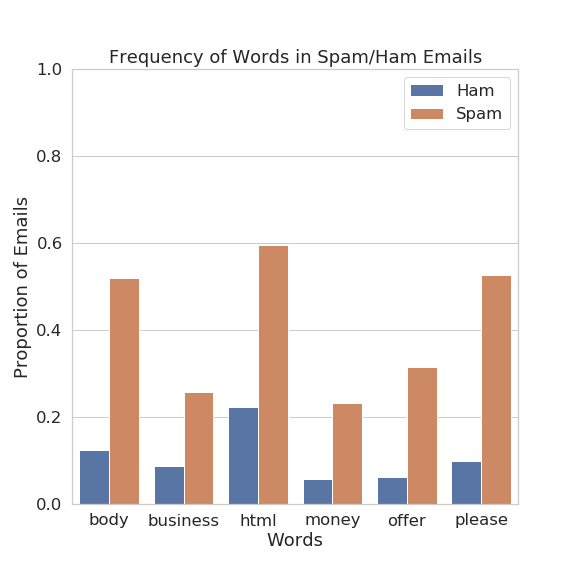
\includegraphics{./images/training_conditional_proportions.png}
\caption{training conditional proportions}
\end{figure}

Hint: - You can use DataFrame's \texttt{.melt} method to "unpivot" a
DataFrame. See the following code cell for example

    \begin{Verbatim}[commandchars=\\\{\}]
{\color{incolor}In [{\color{incolor}13}]:} \PY{k+kn}{from} \PY{n+nn}{IPython}\PY{n+nn}{.}\PY{n+nn}{display} \PY{k}{import} \PY{n}{display}\PY{p}{,} \PY{n}{Markdown}
         \PY{n}{df} \PY{o}{=} \PY{n}{pd}\PY{o}{.}\PY{n}{DataFrame}\PY{p}{(}\PY{p}{\PYZob{}}
             \PY{l+s+s1}{\PYZsq{}}\PY{l+s+s1}{word\PYZus{}1}\PY{l+s+s1}{\PYZsq{}}\PY{p}{:} \PY{p}{[}\PY{l+m+mi}{1}\PY{p}{,} \PY{l+m+mi}{0}\PY{p}{,} \PY{l+m+mi}{1}\PY{p}{,} \PY{l+m+mi}{0}\PY{p}{]}\PY{p}{,}
             \PY{l+s+s1}{\PYZsq{}}\PY{l+s+s1}{word\PYZus{}2}\PY{l+s+s1}{\PYZsq{}}\PY{p}{:} \PY{p}{[}\PY{l+m+mi}{0}\PY{p}{,} \PY{l+m+mi}{1}\PY{p}{,} \PY{l+m+mi}{0}\PY{p}{,} \PY{l+m+mi}{1}\PY{p}{]}\PY{p}{,}
             \PY{l+s+s1}{\PYZsq{}}\PY{l+s+s1}{type}\PY{l+s+s1}{\PYZsq{}}\PY{p}{:} \PY{p}{[}\PY{l+s+s1}{\PYZsq{}}\PY{l+s+s1}{spam}\PY{l+s+s1}{\PYZsq{}}\PY{p}{,} \PY{l+s+s1}{\PYZsq{}}\PY{l+s+s1}{ham}\PY{l+s+s1}{\PYZsq{}}\PY{p}{,} \PY{l+s+s1}{\PYZsq{}}\PY{l+s+s1}{ham}\PY{l+s+s1}{\PYZsq{}}\PY{p}{,} \PY{l+s+s1}{\PYZsq{}}\PY{l+s+s1}{ham}\PY{l+s+s1}{\PYZsq{}}\PY{p}{]}
         \PY{p}{\PYZcb{}}\PY{p}{)}
         \PY{n}{display}\PY{p}{(}\PY{n}{Markdown}\PY{p}{(}\PY{l+s+s2}{\PYZdq{}}\PY{l+s+s2}{\PYZgt{} Our Original DataFrame has some words column and a type column. You can think of each row is a sentence, and the value of 1 or 0 indicates the number of occurances of the word in this sentence.}\PY{l+s+s2}{\PYZdq{}}\PY{p}{)}\PY{p}{)}
         \PY{n}{display}\PY{p}{(}\PY{n}{df}\PY{p}{)}
         \PY{n}{display}\PY{p}{(}\PY{n}{Markdown}\PY{p}{(}\PY{l+s+s2}{\PYZdq{}}\PY{l+s+s2}{\PYZgt{} `melt` will turn columns into variale, notice how `word\PYZus{}1` and `word\PYZus{}2` become `variable`, their values are stoed in the value column}\PY{l+s+s2}{\PYZdq{}}\PY{p}{)}\PY{p}{)}
         \PY{n}{display}\PY{p}{(}\PY{n}{df}\PY{o}{.}\PY{n}{melt}\PY{p}{(}\PY{l+s+s2}{\PYZdq{}}\PY{l+s+s2}{type}\PY{l+s+s2}{\PYZdq{}}\PY{p}{)}\PY{p}{)}
\end{Verbatim}


    \begin{quote}
Our Original DataFrame has some words column and a type column. You can
think of each row is a sentence, and the value of 1 or 0 indicates the
number of occurances of the word in this sentence.
\end{quote}

    
    
    \begin{verbatim}
   type  word_1  word_2
0  spam       1       0
1   ham       0       1
2   ham       1       0
3   ham       0       1
    \end{verbatim}

    
    \begin{quote}
\texttt{melt} will turn columns into variale, notice how
\texttt{word\_1} and \texttt{word\_2} become \texttt{variable}, their
values are stoed in the value column
\end{quote}

    
    
    \begin{verbatim}
   type variable  value
0  spam   word_1      1
1   ham   word_1      0
2   ham   word_1      1
3   ham   word_1      0
4  spam   word_2      0
5   ham   word_2      1
6   ham   word_2      0
7   ham   word_2      1
    \end{verbatim}

    
    \begin{Verbatim}[commandchars=\\\{\}]
{\color{incolor}In [{\color{incolor}14}]:} \PY{n}{train}\PY{o}{=}\PY{n}{train}\PY{o}{.}\PY{n}{reset\PYZus{}index}\PY{p}{(}\PY{p}{)} \PY{c+c1}{\PYZsh{} We must do this in order to preserve the ordering of emails to labels for words\PYZus{}in\PYZus{}texts}
         \PY{c+c1}{\PYZsh{} YOUR CODE HERE}
         \PY{n}{df} \PY{o}{=} \PY{p}{\PYZob{}}\PY{p}{\PYZcb{}}
         \PY{c+c1}{\PYZsh{}word = [\PYZsq{}body\PYZsq{},\PYZsq{}business\PYZsq{},\PYZsq{}html\PYZsq{},\PYZsq{}money\PYZsq{},\PYZsq{}offer\PYZsq{},\PYZsq{}please\PYZsq{}]}
         \PY{n}{word} \PY{o}{=} \PY{p}{[}\PY{l+s+s1}{\PYZsq{}}\PY{l+s+s1}{head}\PY{l+s+s1}{\PYZsq{}}\PY{p}{,}\PY{l+s+s1}{\PYZsq{}}\PY{l+s+s1}{html}\PY{l+s+s1}{\PYZsq{}}\PY{p}{,}\PY{l+s+s1}{\PYZsq{}}\PY{l+s+s1}{class}\PY{l+s+s1}{\PYZsq{}}\PY{p}{,}\PY{l+s+s1}{\PYZsq{}}\PY{l+s+s1}{style}\PY{l+s+s1}{\PYZsq{}}\PY{p}{,}\PY{l+s+s1}{\PYZsq{}}\PY{l+s+s1}{please}\PY{l+s+s1}{\PYZsq{}}\PY{p}{,}\PY{l+s+s1}{\PYZsq{}}\PY{l+s+s1}{increase}\PY{l+s+s1}{\PYZsq{}}\PY{p}{]}
         \PY{n}{word\PYZus{}in\PYZus{}text} \PY{o}{=} \PY{n}{words\PYZus{}in\PYZus{}texts}\PY{p}{(}\PY{n}{word}\PY{p}{,} \PY{n}{train}\PY{p}{[}\PY{l+s+s1}{\PYZsq{}}\PY{l+s+s1}{email}\PY{l+s+s1}{\PYZsq{}}\PY{p}{]}\PY{p}{)}
         \PY{k}{for} \PY{n}{index}\PY{p}{,} \PY{n}{w} \PY{o+ow}{in} \PY{n+nb}{enumerate}\PY{p}{(}\PY{n}{word}\PY{p}{)}\PY{p}{:}
             \PY{n}{df}\PY{p}{[}\PY{n}{w}\PY{p}{]} \PY{o}{=} \PY{p}{[}\PY{n}{word\PYZus{}in\PYZus{}text}\PY{p}{[}\PY{n}{i}\PY{p}{]}\PY{p}{[}\PY{n}{index}\PY{p}{]} \PY{k}{for} \PY{n}{i} \PY{o+ow}{in} \PY{n+nb}{range}\PY{p}{(}\PY{n+nb}{len}\PY{p}{(}\PY{n}{word\PYZus{}in\PYZus{}text}\PY{p}{)}\PY{p}{)}\PY{p}{]}
         \PY{n}{df}\PY{p}{[}\PY{l+s+s1}{\PYZsq{}}\PY{l+s+s1}{type}\PY{l+s+s1}{\PYZsq{}}\PY{p}{]} \PY{o}{=} \PY{p}{[}\PY{l+s+s1}{\PYZsq{}}\PY{l+s+s1}{spam}\PY{l+s+s1}{\PYZsq{}} \PY{k}{if} \PY{n}{train}\PY{o}{.}\PY{n}{iloc}\PY{p}{[}\PY{n}{i}\PY{p}{]}\PY{p}{[}\PY{l+s+s1}{\PYZsq{}}\PY{l+s+s1}{spam}\PY{l+s+s1}{\PYZsq{}}\PY{p}{]}\PY{o}{==}\PY{l+m+mi}{1} \PY{k}{else} \PY{l+s+s1}{\PYZsq{}}\PY{l+s+s1}{ham}\PY{l+s+s1}{\PYZsq{}} \PY{k}{for} \PY{n}{i} \PY{o+ow}{in} \PY{n+nb}{range}\PY{p}{(}\PY{n+nb}{len}\PY{p}{(}\PY{n}{train}\PY{p}{)}\PY{p}{)}\PY{p}{]}
         \PY{n}{df} \PY{o}{=} \PY{n}{pd}\PY{o}{.}\PY{n}{DataFrame}\PY{p}{(}\PY{n}{df}\PY{p}{)}
         \PY{n}{result\PYZus{}df} \PY{o}{=} \PY{n}{df}\PY{o}{.}\PY{n}{melt}\PY{p}{(}\PY{l+s+s2}{\PYZdq{}}\PY{l+s+s2}{type}\PY{l+s+s2}{\PYZdq{}}\PY{p}{)}
         \PY{n}{table} \PY{o}{=} \PY{n}{result\PYZus{}df}\PY{o}{.}\PY{n}{groupby}\PY{p}{(}\PY{p}{[}\PY{l+s+s1}{\PYZsq{}}\PY{l+s+s1}{variable}\PY{l+s+s1}{\PYZsq{}}\PY{p}{,}\PY{l+s+s1}{\PYZsq{}}\PY{l+s+s1}{type}\PY{l+s+s1}{\PYZsq{}}\PY{p}{]}\PY{p}{)}\PY{o}{.}\PY{n}{mean}\PY{p}{(}\PY{p}{)}\PY{o}{.}\PY{n}{reset\PYZus{}index}\PY{p}{(}\PY{p}{[}\PY{l+s+s1}{\PYZsq{}}\PY{l+s+s1}{variable}\PY{l+s+s1}{\PYZsq{}}\PY{p}{,}\PY{l+s+s1}{\PYZsq{}}\PY{l+s+s1}{type}\PY{l+s+s1}{\PYZsq{}}\PY{p}{]}\PY{p}{)}
         
         \PY{n}{fig}\PY{p}{,} \PY{n}{ax} \PY{o}{=} \PY{n}{plt}\PY{o}{.}\PY{n}{subplots}\PY{p}{(}\PY{n}{figsize}\PY{o}{=}\PY{p}{(}\PY{l+m+mi}{8}\PY{p}{,}\PY{l+m+mi}{8}\PY{p}{)}\PY{p}{)}
         \PY{n}{ax} \PY{o}{=} \PY{n}{sns}\PY{o}{.}\PY{n}{barplot}\PY{p}{(}\PY{n}{x} \PY{o}{=} \PY{l+s+s1}{\PYZsq{}}\PY{l+s+s1}{variable}\PY{l+s+s1}{\PYZsq{}}\PY{p}{,}\PY{n}{y} \PY{o}{=} \PY{l+s+s1}{\PYZsq{}}\PY{l+s+s1}{value}\PY{l+s+s1}{\PYZsq{}}\PY{p}{,} \PY{n}{hue}\PY{o}{=}\PY{l+s+s1}{\PYZsq{}}\PY{l+s+s1}{type}\PY{l+s+s1}{\PYZsq{}}\PY{p}{,} \PY{n}{data}\PY{o}{=}\PY{n}{table}\PY{p}{)}
         \PY{n}{ax}\PY{o}{.}\PY{n}{set}\PY{p}{(}\PY{n}{ylim}\PY{o}{=}\PY{p}{(}\PY{l+m+mi}{0}\PY{p}{,} \PY{l+m+mf}{1.0}\PY{p}{)}\PY{p}{)}
         \PY{n}{ax}\PY{o}{.}\PY{n}{set\PYZus{}title}\PY{p}{(}\PY{l+s+s1}{\PYZsq{}}\PY{l+s+s1}{Frequency of Words in Spam/Ham Emails}\PY{l+s+s1}{\PYZsq{}}\PY{p}{)}
         \PY{n}{ax}\PY{o}{.}\PY{n}{set}\PY{p}{(}\PY{n}{xlabel}\PY{o}{=}\PY{l+s+s1}{\PYZsq{}}\PY{l+s+s1}{Words}\PY{l+s+s1}{\PYZsq{}}\PY{p}{,} \PY{n}{ylabel}\PY{o}{=}\PY{l+s+s1}{\PYZsq{}}\PY{l+s+s1}{Proportion of Emails}\PY{l+s+s1}{\PYZsq{}}\PY{p}{)}
\end{Verbatim}


\begin{Verbatim}[commandchars=\\\{\}]
{\color{outcolor}Out[{\color{outcolor}14}]:} [Text(0,0.5,'Proportion of Emails'), Text(0.5,0,'Words')]
\end{Verbatim}
            
    \begin{center}
    \adjustimage{max size={0.9\linewidth}{0.9\paperheight}}{output_27_1.png}
    \end{center}
    { \hspace*{\fill} \\}
    
    \section{Question 3b}\label{question-3b}

When the feature is binary, it makes sense (as in the previous question)
to compare the proportion of 1s in the two classes of email. Otherwise,
if the feature can take on many values, it makes sense to compare the
distribution under spam to the distribution under ham. Create a
\emph{class conditional density plot} like the one below (which was
created using \texttt{sns.distplot}), comparing the distribution of a
feature among all spam emails to the distribution of the same feature
among all ham emails. You should use your training set (after
splitting). \textbf{You may use the length of the email body or create
your own feature.} If using length of the email body, please set the
xlim to 50000.

\begin{figure}
\centering
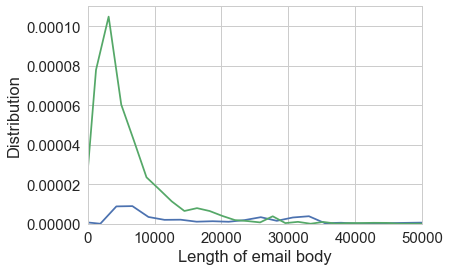
\includegraphics{./images/training_conditional_densities2.png}
\caption{training conditional densities}
\end{figure}

    \begin{Verbatim}[commandchars=\\\{\}]
{\color{incolor}In [{\color{incolor}15}]:} \PY{c+c1}{\PYZsh{} YOUR CODE HERE}
         \PY{n}{train\PYZus{}spam\PYZus{}len} \PY{o}{=} \PY{p}{[}\PY{n+nb}{len}\PY{p}{(}\PY{n}{train}\PY{o}{.}\PY{n}{iloc}\PY{p}{[}\PY{n}{i}\PY{p}{]}\PY{p}{[}\PY{l+s+s1}{\PYZsq{}}\PY{l+s+s1}{email}\PY{l+s+s1}{\PYZsq{}}\PY{p}{]}\PY{p}{)} \PY{k}{for} \PY{n}{i} \PY{o+ow}{in} \PY{n+nb}{range}\PY{p}{(}\PY{n+nb}{len}\PY{p}{(}\PY{n}{train}\PY{p}{)}\PY{p}{)} 
                           \PY{k}{if} \PY{n}{train}\PY{o}{.}\PY{n}{iloc}\PY{p}{[}\PY{n}{i}\PY{p}{]}\PY{p}{[}\PY{l+s+s1}{\PYZsq{}}\PY{l+s+s1}{spam}\PY{l+s+s1}{\PYZsq{}}\PY{p}{]}\PY{o}{==}\PY{l+m+mi}{1}\PY{p}{]}
         \PY{n}{train\PYZus{}ham\PYZus{}len} \PY{o}{=} \PY{p}{[}\PY{n+nb}{len}\PY{p}{(}\PY{n}{train}\PY{o}{.}\PY{n}{iloc}\PY{p}{[}\PY{n}{i}\PY{p}{]}\PY{p}{[}\PY{l+s+s1}{\PYZsq{}}\PY{l+s+s1}{email}\PY{l+s+s1}{\PYZsq{}}\PY{p}{]}\PY{p}{)} \PY{k}{for} \PY{n}{i} \PY{o+ow}{in} \PY{n+nb}{range}\PY{p}{(}\PY{n+nb}{len}\PY{p}{(}\PY{n}{train}\PY{p}{)}\PY{p}{)} 
                           \PY{k}{if} \PY{n}{train}\PY{o}{.}\PY{n}{iloc}\PY{p}{[}\PY{n}{i}\PY{p}{]}\PY{p}{[}\PY{l+s+s1}{\PYZsq{}}\PY{l+s+s1}{spam}\PY{l+s+s1}{\PYZsq{}}\PY{p}{]}\PY{o}{==}\PY{l+m+mi}{0}\PY{p}{]}
         \PY{n}{ax} \PY{o}{=} \PY{n}{sns}\PY{o}{.}\PY{n}{distplot}\PY{p}{(}\PY{n}{train\PYZus{}spam\PYZus{}len}\PY{p}{,}\PY{n}{hist}\PY{o}{=}\PY{k+kc}{False}\PY{p}{,}\PY{n}{color}\PY{o}{=}\PY{l+s+s1}{\PYZsq{}}\PY{l+s+s1}{g}\PY{l+s+s1}{\PYZsq{}}\PY{p}{)}
         \PY{n}{ax} \PY{o}{=} \PY{n}{sns}\PY{o}{.}\PY{n}{distplot}\PY{p}{(}\PY{n}{train\PYZus{}ham\PYZus{}len}\PY{p}{,}\PY{n}{hist}\PY{o}{=}\PY{k+kc}{False}\PY{p}{,}\PY{n}{color}\PY{o}{=}\PY{l+s+s1}{\PYZsq{}}\PY{l+s+s1}{b}\PY{l+s+s1}{\PYZsq{}}\PY{p}{)}
         \PY{n}{ax}\PY{o}{.}\PY{n}{set}\PY{p}{(}\PY{n}{xlim}\PY{o}{=}\PY{p}{(}\PY{l+m+mi}{0}\PY{p}{,}\PY{l+m+mi}{50000}\PY{p}{)}\PY{p}{)}
         \PY{n}{ax}\PY{o}{.}\PY{n}{set}\PY{p}{(}\PY{n}{xlabel}\PY{o}{=}\PY{l+s+s1}{\PYZsq{}}\PY{l+s+s1}{Length of email body}\PY{l+s+s1}{\PYZsq{}}\PY{p}{,} \PY{n}{ylabel}\PY{o}{=}\PY{l+s+s1}{\PYZsq{}}\PY{l+s+s1}{Distribution}\PY{l+s+s1}{\PYZsq{}}\PY{p}{)}
\end{Verbatim}


\begin{Verbatim}[commandchars=\\\{\}]
{\color{outcolor}Out[{\color{outcolor}15}]:} [Text(0,0.5,'Distribution'), Text(0.5,0,'Length of email body')]
\end{Verbatim}
            
    \begin{center}
    \adjustimage{max size={0.9\linewidth}{0.9\paperheight}}{output_29_1.png}
    \end{center}
    { \hspace*{\fill} \\}
    
    \section{Basic Classification}\label{basic-classification}

Notice that the output of
\texttt{words\_in\_texts(words,\ train{[}\textquotesingle{}email\textquotesingle{}{]})}
is a numeric matrix containing features for each email. This means we
can use it directly to train a classifier!

    \section{Question 4}\label{question-4}

We've given you 5 words that might be useful as features to distinguish
spam/ham emails. Use these words as well as the \texttt{train} DataFrame
to create two NumPy arrays: \texttt{Phi\_train} and \texttt{Y\_train}.

\texttt{Phi\_train} should be a matrix of 0s and 1s created by using
your \texttt{words\_in\_texts} function on all the emails in the
training set.

\texttt{Y\_train} should be a vector of the correct labels for each
email in the training set.

    \begin{Verbatim}[commandchars=\\\{\}]
{\color{incolor}In [{\color{incolor}16}]:} \PY{n}{some\PYZus{}words} \PY{o}{=} \PY{p}{[}\PY{l+s+s1}{\PYZsq{}}\PY{l+s+s1}{drug}\PY{l+s+s1}{\PYZsq{}}\PY{p}{,} \PY{l+s+s1}{\PYZsq{}}\PY{l+s+s1}{bank}\PY{l+s+s1}{\PYZsq{}}\PY{p}{,} \PY{l+s+s1}{\PYZsq{}}\PY{l+s+s1}{prescription}\PY{l+s+s1}{\PYZsq{}}\PY{p}{,} \PY{l+s+s1}{\PYZsq{}}\PY{l+s+s1}{memo}\PY{l+s+s1}{\PYZsq{}}\PY{p}{,} \PY{l+s+s1}{\PYZsq{}}\PY{l+s+s1}{private}\PY{l+s+s1}{\PYZsq{}}\PY{p}{]}
         
         \PY{n}{Phi\PYZus{}train} \PY{o}{=} \PY{n}{words\PYZus{}in\PYZus{}texts}\PY{p}{(}\PY{n}{some\PYZus{}words}\PY{p}{,}\PY{n}{train}\PY{p}{[}\PY{l+s+s1}{\PYZsq{}}\PY{l+s+s1}{email}\PY{l+s+s1}{\PYZsq{}}\PY{p}{]}\PY{p}{)}
         \PY{n}{Y\PYZus{}train} \PY{o}{=} \PY{n}{train}\PY{p}{[}\PY{l+s+s1}{\PYZsq{}}\PY{l+s+s1}{spam}\PY{l+s+s1}{\PYZsq{}}\PY{p}{]}
         
         \PY{c+c1}{\PYZsh{} YOUR CODE HERE}
         
         \PY{n}{Phi\PYZus{}train}\PY{p}{[}\PY{p}{:}\PY{l+m+mi}{5}\PY{p}{]}\PY{p}{,} \PY{n}{Y\PYZus{}train}\PY{p}{[}\PY{p}{:}\PY{l+m+mi}{5}\PY{p}{]}
\end{Verbatim}


\begin{Verbatim}[commandchars=\\\{\}]
{\color{outcolor}Out[{\color{outcolor}16}]:} (array([[0, 0, 0, 0, 0],
                 [0, 0, 0, 0, 0],
                 [0, 0, 0, 0, 0],
                 [0, 0, 0, 0, 0],
                 [0, 0, 0, 1, 0]]), 0    0
          1    0
          2    0
          3    0
          4    0
          Name: spam, dtype: int64)
\end{Verbatim}
            
    \begin{Verbatim}[commandchars=\\\{\}]
{\color{incolor}In [{\color{incolor}17}]:} \PY{k}{assert} \PY{n}{np}\PY{o}{.}\PY{n}{all}\PY{p}{(}\PY{n}{np}\PY{o}{.}\PY{n}{unique}\PY{p}{(}\PY{n}{Phi\PYZus{}train}\PY{p}{)} \PY{o}{==} \PY{n}{np}\PY{o}{.}\PY{n}{array}\PY{p}{(}\PY{p}{[}\PY{l+m+mi}{0}\PY{p}{,} \PY{l+m+mi}{1}\PY{p}{]}\PY{p}{)}\PY{p}{)}
         \PY{k}{assert} \PY{n}{np}\PY{o}{.}\PY{n}{all}\PY{p}{(}\PY{n}{np}\PY{o}{.}\PY{n}{unique}\PY{p}{(}\PY{n}{Y\PYZus{}train}\PY{p}{)} \PY{o}{==} \PY{n}{np}\PY{o}{.}\PY{n}{array}\PY{p}{(}\PY{p}{[}\PY{l+m+mi}{0}\PY{p}{,} \PY{l+m+mi}{1}\PY{p}{]}\PY{p}{)}\PY{p}{)}
         \PY{k}{assert} \PY{n}{Phi\PYZus{}train}\PY{o}{.}\PY{n}{shape}\PY{p}{[}\PY{l+m+mi}{0}\PY{p}{]} \PY{o}{==} \PY{n}{Y\PYZus{}train}\PY{o}{.}\PY{n}{shape}\PY{p}{[}\PY{l+m+mi}{0}\PY{p}{]}
         \PY{k}{assert} \PY{n}{Phi\PYZus{}train}\PY{o}{.}\PY{n}{shape}\PY{p}{[}\PY{l+m+mi}{1}\PY{p}{]} \PY{o}{==} \PY{n+nb}{len}\PY{p}{(}\PY{n}{some\PYZus{}words}\PY{p}{)}
\end{Verbatim}


    \section{Question 5}\label{question-5}

Now we have matrices we can give to scikit-learn! Using the
\href{http://scikit-learn.org/stable/modules/generated/sklearn.linear_model.LogisticRegression.html}{\texttt{LogisticRegression}}
classifier, train a logistic regression model using \texttt{Phi\_train}
and \texttt{Y\_train}. Then, output the accuracy of the model (on the
training data) in the cell below. You should get an accuracy of around
0.75.

    \begin{Verbatim}[commandchars=\\\{\}]
{\color{incolor}In [{\color{incolor}18}]:} \PY{k+kn}{from} \PY{n+nn}{sklearn}\PY{n+nn}{.}\PY{n+nn}{linear\PYZus{}model} \PY{k}{import} \PY{n}{LogisticRegression}
         
         \PY{n}{model} \PY{o}{=} \PY{n}{LogisticRegression}\PY{p}{(}\PY{p}{)}
         \PY{n}{model}\PY{o}{.}\PY{n}{fit}\PY{p}{(}\PY{n}{Phi\PYZus{}train}\PY{p}{,} \PY{n}{Y\PYZus{}train}\PY{p}{)}
         \PY{n}{training\PYZus{}accuracy} \PY{o}{=} \PY{n}{model}\PY{o}{.}\PY{n}{score}\PY{p}{(}\PY{n}{Phi\PYZus{}train}\PY{p}{,} \PY{n}{Y\PYZus{}train}\PY{p}{)}
         \PY{n}{training\PYZus{}accuracy}
         
         \PY{c+c1}{\PYZsh{} YOUR CODE HERE}
\end{Verbatim}


\begin{Verbatim}[commandchars=\\\{\}]
{\color{outcolor}Out[{\color{outcolor}18}]:} 0.75762012511646482
\end{Verbatim}
            
    \begin{Verbatim}[commandchars=\\\{\}]
{\color{incolor}In [{\color{incolor}19}]:} \PY{k}{assert} \PY{n}{training\PYZus{}accuracy} \PY{o}{\PYZgt{}} \PY{l+m+mf}{0.72}
\end{Verbatim}


    \section{Question 6}\label{question-6}

That doesn't seem too shabby! But the classifier you made above isn't as
good as this might lead us to believe. First, we are validating on the
training set, which may lead to a misleading accuracy measure,
especially if we used the training set to identify discriminative
features. In future parts of this analysis, it will be safer to hold out
some of our data for model validation and comparison.

Presumably, our classifier will be used for \textbf{filtering}, i.e.
preventing messages labeled \texttt{spam} from reaching someone's inbox.
Since we are trying There are two kinds of errors we can make: - False
positive (FP): a ham email gets flagged as spam and filtered out of the
inbox. - False negative (FN): a spam email gets mislabeled as ham and
ends up in the inbox.

These definitions depend both on the true labels and the predicted
labels. False positives and false negatives may be of differing
importance, leading us to consider more ways of evaluating a classifier,
in addition to overall accuracy:

\textbf{Precision} measures the proportion
\(\frac{\text{TP}}{\text{TP} + \text{FP}}\) of emails flagged as spam
that are actually spam.

\textbf{Recall} measures the proportion
\(\frac{\text{TP}}{\text{TP} + \text{FN}}\) of spam emails that were
correctly flagged as spam.

\textbf{False-alarm rate} measures the proportion
\(\frac{\text{FP}}{\text{FP} + \text{TN}}\) of ham emails that were
incorrectly flagged as spam.

The following image might help:

Note that a true positive (TP) is a spam email that is classified as
spam, and a true negative (TN) is a ham email that is classified as ham.
Answer the following questions in the cells below:

\begin{itemize}
\item
  \begin{enumerate}
  \def\labelenumi{(\alph{enumi})}
  \tightlist
  \item
    Suppose we have a classifier that just predicts 0 (ham) for every
    email. How many false positives are there? How many false negatives
    are there? Provide specific numbers using the training data from
    Question 4.
  \end{enumerate}
\item
  \begin{enumerate}
  \def\labelenumi{(\alph{enumi})}
  \setcounter{enumi}{1}
  \tightlist
  \item
    Suppose we have a classifier that just predicts 0 (ham) for every
    email. What is its accuracy on the training set? What is its recall
    on the training set?
  \end{enumerate}
\item
  \begin{enumerate}
  \def\labelenumi{(\alph{enumi})}
  \setcounter{enumi}{2}
  \tightlist
  \item
    What are the precision, recall, and false-alarm rate of the logistic
    regression classifier in Question 5? Are there more false positives
    or false negatives?
  \end{enumerate}
\item
  \begin{enumerate}
  \def\labelenumi{(\alph{enumi})}
  \setcounter{enumi}{3}
  \tightlist
  \item
    Our logistic regression classifier got 75.6\% prediction accuracy
    (number of correct predictions / total). How does this compare with
    predicting 0 for every email?
  \end{enumerate}
\item
  \begin{enumerate}
  \def\labelenumi{(\alph{enumi})}
  \setcounter{enumi}{4}
  \tightlist
  \item
    Given the word features we gave you above, name one reason this
    classifier is performing poorly.
  \end{enumerate}
\item
  \begin{enumerate}
  \def\labelenumi{(\alph{enumi})}
  \setcounter{enumi}{5}
  \tightlist
  \item
    Which of these two classifiers would you prefer for a spam filter
    and why? (N.B. there is no "right answer" here but be thoughtful in
    your reasoning).
  \end{enumerate}
\end{itemize}

    \begin{Verbatim}[commandchars=\\\{\}]
{\color{incolor}In [{\color{incolor}20}]:} \PY{c+c1}{\PYZsh{} provide number of FP and FN, respectively,}
         \PY{c+c1}{\PYZsh{} for a classifier that always predicts 0 (never predicts positive...)}
         \PY{n}{zero\PYZus{}predictor\PYZus{}fp} \PY{o}{=} \PY{l+m+mi}{0}
         \PY{n}{zero\PYZus{}predictor\PYZus{}fn} \PY{o}{=} \PY{n}{Y\PYZus{}train}\PY{o}{.}\PY{n}{sum}\PY{p}{(}\PY{p}{)}
         \PY{c+c1}{\PYZsh{}1918}
         
         \PY{c+c1}{\PYZsh{} YOUR CODE HERE}
\end{Verbatim}


    \begin{Verbatim}[commandchars=\\\{\}]
{\color{incolor}In [{\color{incolor}21}]:} \PY{c+c1}{\PYZsh{} This is a cell with just a comment but don\PYZsq{}t delete me if you want to get credit.}
\end{Verbatim}


    \begin{Verbatim}[commandchars=\\\{\}]
{\color{incolor}In [{\color{incolor}22}]:} \PY{c+c1}{\PYZsh{} provide training accuracy \PYZam{} recall, respectively,}
         \PY{c+c1}{\PYZsh{} for a classifier that always predicts 0}
         \PY{n}{zero\PYZus{}predictor\PYZus{}acc} \PY{o}{=} \PY{p}{(}\PY{n+nb}{len}\PY{p}{(}\PY{n}{Y\PYZus{}train}\PY{p}{)}\PY{o}{\PYZhy{}}\PY{n}{Y\PYZus{}train}\PY{o}{.}\PY{n}{sum}\PY{p}{(}\PY{p}{)}\PY{p}{)}\PY{o}{/} \PY{n+nb}{len}\PY{p}{(}\PY{n}{Y\PYZus{}train}\PY{p}{)}
         \PY{n}{zero\PYZus{}predictor\PYZus{}recall} \PY{o}{=} \PY{l+m+mi}{0}
         \PY{n+nb}{print}\PY{p}{(}\PY{n}{zero\PYZus{}predictor\PYZus{}acc}\PY{p}{)}
         \PY{c+c1}{\PYZsh{} YOUR CODE HERE}
\end{Verbatim}


    \begin{Verbatim}[commandchars=\\\{\}]
0.744709170771

    \end{Verbatim}

    \begin{Verbatim}[commandchars=\\\{\}]
{\color{incolor}In [{\color{incolor}23}]:} \PY{c+c1}{\PYZsh{} This is a cell with just a comment but don\PYZsq{}t delete me if you want to get credit.}
\end{Verbatim}


    \begin{Verbatim}[commandchars=\\\{\}]
{\color{incolor}In [{\color{incolor}24}]:} \PY{c+c1}{\PYZsh{} provide training accuracy \PYZam{} recall, respectively,}
         \PY{c+c1}{\PYZsh{} for logistic regression classifier from question 5}
         \PY{n}{Y\PYZus{}pred\PYZus{}train} \PY{o}{=} \PY{n}{model}\PY{o}{.}\PY{n}{predict}\PY{p}{(}\PY{n}{Phi\PYZus{}train}\PY{p}{)}
         \PY{n}{TP} \PY{o}{=} \PY{n+nb}{sum}\PY{p}{(}\PY{p}{[}\PY{l+m+mi}{1} \PY{k}{for} \PY{n}{i} \PY{o+ow}{in} \PY{n+nb}{range}\PY{p}{(}\PY{n+nb}{len}\PY{p}{(}\PY{n}{Y\PYZus{}train}\PY{p}{)}\PY{p}{)} \PY{k}{if} \PY{n}{Y\PYZus{}pred\PYZus{}train}\PY{p}{[}\PY{n}{i}\PY{p}{]}\PY{o}{==}\PY{l+m+mi}{1} \PY{o+ow}{and} \PY{n}{Y\PYZus{}train}\PY{p}{[}\PY{n}{i}\PY{p}{]}\PY{o}{==}\PY{l+m+mi}{1}\PY{p}{]}\PY{p}{)}
         \PY{n}{TN} \PY{o}{=} \PY{n+nb}{sum}\PY{p}{(}\PY{p}{[}\PY{l+m+mi}{1} \PY{k}{for} \PY{n}{i} \PY{o+ow}{in} \PY{n+nb}{range}\PY{p}{(}\PY{n+nb}{len}\PY{p}{(}\PY{n}{Y\PYZus{}train}\PY{p}{)}\PY{p}{)} \PY{k}{if} \PY{n}{Y\PYZus{}pred\PYZus{}train}\PY{p}{[}\PY{n}{i}\PY{p}{]}\PY{o}{==}\PY{l+m+mi}{0} \PY{o+ow}{and} \PY{n}{Y\PYZus{}train}\PY{p}{[}\PY{n}{i}\PY{p}{]}\PY{o}{==}\PY{l+m+mi}{0}\PY{p}{]}\PY{p}{)}
         \PY{n}{FP} \PY{o}{=} \PY{n+nb}{sum}\PY{p}{(}\PY{p}{[}\PY{l+m+mi}{1} \PY{k}{for} \PY{n}{i} \PY{o+ow}{in} \PY{n+nb}{range}\PY{p}{(}\PY{n+nb}{len}\PY{p}{(}\PY{n}{Y\PYZus{}train}\PY{p}{)}\PY{p}{)} \PY{k}{if} \PY{n}{Y\PYZus{}pred\PYZus{}train}\PY{p}{[}\PY{n}{i}\PY{p}{]}\PY{o}{==}\PY{l+m+mi}{1} \PY{o+ow}{and} \PY{n}{Y\PYZus{}train}\PY{p}{[}\PY{n}{i}\PY{p}{]}\PY{o}{==}\PY{l+m+mi}{0}\PY{p}{]}\PY{p}{)}
         \PY{n}{FN} \PY{o}{=} \PY{n+nb}{sum}\PY{p}{(}\PY{p}{[}\PY{l+m+mi}{1} \PY{k}{for} \PY{n}{i} \PY{o+ow}{in} \PY{n+nb}{range}\PY{p}{(}\PY{n+nb}{len}\PY{p}{(}\PY{n}{Y\PYZus{}train}\PY{p}{)}\PY{p}{)} \PY{k}{if} \PY{n}{Y\PYZus{}pred\PYZus{}train}\PY{p}{[}\PY{n}{i}\PY{p}{]}\PY{o}{==}\PY{l+m+mi}{0} \PY{o+ow}{and} \PY{n}{Y\PYZus{}train}\PY{p}{[}\PY{n}{i}\PY{p}{]}\PY{o}{==}\PY{l+m+mi}{1}\PY{p}{]}\PY{p}{)}
         
         \PY{n}{logistic\PYZus{}predictor\PYZus{}precision} \PY{o}{=} \PY{n}{TP}\PY{o}{/}\PY{p}{(}\PY{n}{TP}\PY{o}{+}\PY{n}{FP}\PY{p}{)}
         \PY{n}{logistic\PYZus{}predictor\PYZus{}recall} \PY{o}{=} \PY{n}{TP}\PY{o}{/}\PY{p}{(}\PY{n}{TP}\PY{o}{+}\PY{n}{FN}\PY{p}{)}
         \PY{n}{logistic\PYZus{}predictor\PYZus{}far} \PY{o}{=} \PY{n}{FP}\PY{o}{/}\PY{p}{(}\PY{n}{FP}\PY{o}{+}\PY{n}{TN}\PY{p}{)}
         \PY{n+nb}{print}\PY{p}{(}\PY{l+s+s1}{\PYZsq{}}\PY{l+s+s1}{Precision is: }\PY{l+s+si}{\PYZpc{}s}\PY{l+s+s1}{\PYZsq{}}\PY{o}{\PYZpc{}}\PY{k}{logistic\PYZus{}predictor\PYZus{}precision})
         \PY{n+nb}{print}\PY{p}{(}\PY{l+s+s1}{\PYZsq{}}\PY{l+s+s1}{Recall is: }\PY{l+s+si}{\PYZpc{}s}\PY{l+s+s1}{\PYZsq{}}\PY{o}{\PYZpc{}}\PY{k}{logistic\PYZus{}predictor\PYZus{}recall})
         \PY{n+nb}{print}\PY{p}{(}\PY{l+s+s1}{\PYZsq{}}\PY{l+s+s1}{False\PYZhy{}alarm rate is: }\PY{l+s+si}{\PYZpc{}s}\PY{l+s+s1}{\PYZsq{}}\PY{o}{\PYZpc{}}\PY{k}{logistic\PYZus{}predictor\PYZus{}far})
         \PY{c+c1}{\PYZsh{} YOUR CODE HERE}
\end{Verbatim}


    \begin{Verbatim}[commandchars=\\\{\}]
Precision is: 0.6422287390029325
Recall is: 0.11418143899895725
False-alarm rate is: 0.021805183199285077

    \end{Verbatim}

    \begin{Verbatim}[commandchars=\\\{\}]
{\color{incolor}In [{\color{incolor}25}]:} \PY{c+c1}{\PYZsh{}Are there more false positives or false negatives?}
         \PY{n+nb}{print}\PY{p}{(}\PY{n}{FP}\PY{p}{)}
         \PY{n+nb}{print}\PY{p}{(}\PY{n}{FN}\PY{p}{)}
\end{Verbatim}


    \begin{Verbatim}[commandchars=\\\{\}]
122
1699

    \end{Verbatim}

    The above result suggests that there are more false negatives.

    \begin{Verbatim}[commandchars=\\\{\}]
{\color{incolor}In [{\color{incolor}26}]:} \PY{c+c1}{\PYZsh{} This is a cell with just a comment but don\PYZsq{}t delete me if you want to get credit.}
\end{Verbatim}


    \begin{itemize}
\item
  \begin{enumerate}
  \def\labelenumi{(\alph{enumi})}
  \setcounter{enumi}{3}
  \tightlist
  \item
    Our logistic regression classifier got 75.6\% prediction accuracy
    (number of correct predictions / total). How does this compare with
    predicting 0 for every email?
  \end{enumerate}
\end{itemize}

    \begin{Verbatim}[commandchars=\\\{\}]
{\color{incolor}In [{\color{incolor}27}]:} \PY{c+c1}{\PYZsh{} for a classifier that always predicts 0}
         \PY{n}{zero\PYZus{}accuracy} \PY{o}{=} \PY{p}{(}\PY{n+nb}{len}\PY{p}{(}\PY{n}{Y\PYZus{}train}\PY{p}{)}\PY{o}{\PYZhy{}}\PY{n}{Y\PYZus{}train}\PY{o}{.}\PY{n}{sum}\PY{p}{(}\PY{p}{)}\PY{p}{)}\PY{o}{/} \PY{n+nb}{len}\PY{p}{(}\PY{n}{Y\PYZus{}train}\PY{p}{)}
         \PY{n}{zero\PYZus{}accuracy}
\end{Verbatim}


\begin{Verbatim}[commandchars=\\\{\}]
{\color{outcolor}Out[{\color{outcolor}27}]:} 0.74470917077066423
\end{Verbatim}
            
    Our logistic regression classifier got 75.6\% prediction accuracy, which
is only a little higher than that of a classifier that always predicts
0.

    \begin{itemize}
\item
  \begin{enumerate}
  \def\labelenumi{(\alph{enumi})}
  \setcounter{enumi}{4}
  \tightlist
  \item
    Given the word features we gave you above, name one reason this
    classifier is performing poorly.
  \end{enumerate}
\end{itemize}

    \begin{Verbatim}[commandchars=\\\{\}]
{\color{incolor}In [{\color{incolor}28}]:} \PY{n}{df} \PY{o}{=} \PY{p}{\PYZob{}}\PY{p}{\PYZcb{}}
         \PY{c+c1}{\PYZsh{}word = [\PYZsq{}body\PYZsq{},\PYZsq{}business\PYZsq{},\PYZsq{}html\PYZsq{},\PYZsq{}money\PYZsq{},\PYZsq{}offer\PYZsq{},\PYZsq{}please\PYZsq{}]}
         \PY{n}{word} \PY{o}{=} \PY{n}{some\PYZus{}words}
         \PY{n}{word\PYZus{}in\PYZus{}text} \PY{o}{=} \PY{n}{words\PYZus{}in\PYZus{}texts}\PY{p}{(}\PY{n}{word}\PY{p}{,} \PY{n}{train}\PY{p}{[}\PY{l+s+s1}{\PYZsq{}}\PY{l+s+s1}{email}\PY{l+s+s1}{\PYZsq{}}\PY{p}{]}\PY{p}{)}
         \PY{k}{for} \PY{n}{index}\PY{p}{,} \PY{n}{w} \PY{o+ow}{in} \PY{n+nb}{enumerate}\PY{p}{(}\PY{n}{word}\PY{p}{)}\PY{p}{:}
             \PY{n}{df}\PY{p}{[}\PY{n}{w}\PY{p}{]} \PY{o}{=} \PY{p}{[}\PY{n}{word\PYZus{}in\PYZus{}text}\PY{p}{[}\PY{n}{i}\PY{p}{]}\PY{p}{[}\PY{n}{index}\PY{p}{]} \PY{k}{for} \PY{n}{i} \PY{o+ow}{in} \PY{n+nb}{range}\PY{p}{(}\PY{n+nb}{len}\PY{p}{(}\PY{n}{word\PYZus{}in\PYZus{}text}\PY{p}{)}\PY{p}{)}\PY{p}{]}
         \PY{n}{df}\PY{p}{[}\PY{l+s+s1}{\PYZsq{}}\PY{l+s+s1}{type}\PY{l+s+s1}{\PYZsq{}}\PY{p}{]} \PY{o}{=} \PY{p}{[}\PY{l+s+s1}{\PYZsq{}}\PY{l+s+s1}{spam}\PY{l+s+s1}{\PYZsq{}} \PY{k}{if} \PY{n}{train}\PY{o}{.}\PY{n}{iloc}\PY{p}{[}\PY{n}{i}\PY{p}{]}\PY{p}{[}\PY{l+s+s1}{\PYZsq{}}\PY{l+s+s1}{spam}\PY{l+s+s1}{\PYZsq{}}\PY{p}{]}\PY{o}{==}\PY{l+m+mi}{1} \PY{k}{else} \PY{l+s+s1}{\PYZsq{}}\PY{l+s+s1}{ham}\PY{l+s+s1}{\PYZsq{}} \PY{k}{for} \PY{n}{i} \PY{o+ow}{in} \PY{n+nb}{range}\PY{p}{(}\PY{n+nb}{len}\PY{p}{(}\PY{n}{train}\PY{p}{)}\PY{p}{)}\PY{p}{]}
         \PY{n}{df} \PY{o}{=} \PY{n}{pd}\PY{o}{.}\PY{n}{DataFrame}\PY{p}{(}\PY{n}{df}\PY{p}{)}
         \PY{n}{result\PYZus{}df} \PY{o}{=} \PY{n}{df}\PY{o}{.}\PY{n}{melt}\PY{p}{(}\PY{l+s+s2}{\PYZdq{}}\PY{l+s+s2}{type}\PY{l+s+s2}{\PYZdq{}}\PY{p}{)}
         \PY{n}{table} \PY{o}{=} \PY{n}{result\PYZus{}df}\PY{o}{.}\PY{n}{groupby}\PY{p}{(}\PY{p}{[}\PY{l+s+s1}{\PYZsq{}}\PY{l+s+s1}{variable}\PY{l+s+s1}{\PYZsq{}}\PY{p}{,}\PY{l+s+s1}{\PYZsq{}}\PY{l+s+s1}{type}\PY{l+s+s1}{\PYZsq{}}\PY{p}{]}\PY{p}{)}\PY{o}{.}\PY{n}{mean}\PY{p}{(}\PY{p}{)}\PY{o}{.}\PY{n}{reset\PYZus{}index}\PY{p}{(}\PY{p}{[}\PY{l+s+s1}{\PYZsq{}}\PY{l+s+s1}{variable}\PY{l+s+s1}{\PYZsq{}}\PY{p}{,}\PY{l+s+s1}{\PYZsq{}}\PY{l+s+s1}{type}\PY{l+s+s1}{\PYZsq{}}\PY{p}{]}\PY{p}{)}
         
         \PY{n}{fig}\PY{p}{,} \PY{n}{ax} \PY{o}{=} \PY{n}{plt}\PY{o}{.}\PY{n}{subplots}\PY{p}{(}\PY{n}{figsize}\PY{o}{=}\PY{p}{(}\PY{l+m+mi}{8}\PY{p}{,}\PY{l+m+mi}{8}\PY{p}{)}\PY{p}{)}
         \PY{n}{ax} \PY{o}{=} \PY{n}{sns}\PY{o}{.}\PY{n}{barplot}\PY{p}{(}\PY{n}{x} \PY{o}{=} \PY{l+s+s1}{\PYZsq{}}\PY{l+s+s1}{variable}\PY{l+s+s1}{\PYZsq{}}\PY{p}{,}\PY{n}{y} \PY{o}{=} \PY{l+s+s1}{\PYZsq{}}\PY{l+s+s1}{value}\PY{l+s+s1}{\PYZsq{}}\PY{p}{,} \PY{n}{hue}\PY{o}{=}\PY{l+s+s1}{\PYZsq{}}\PY{l+s+s1}{type}\PY{l+s+s1}{\PYZsq{}}\PY{p}{,} \PY{n}{data}\PY{o}{=}\PY{n}{table}\PY{p}{)}
         \PY{n}{ax}\PY{o}{.}\PY{n}{set}\PY{p}{(}\PY{n}{ylim}\PY{o}{=}\PY{p}{(}\PY{l+m+mi}{0}\PY{p}{,} \PY{l+m+mf}{1.0}\PY{p}{)}\PY{p}{)}
         \PY{n}{ax}\PY{o}{.}\PY{n}{set\PYZus{}title}\PY{p}{(}\PY{l+s+s1}{\PYZsq{}}\PY{l+s+s1}{Frequency of Words in Spam/Ham Emails}\PY{l+s+s1}{\PYZsq{}}\PY{p}{)}
         \PY{n}{ax}\PY{o}{.}\PY{n}{set}\PY{p}{(}\PY{n}{xlabel}\PY{o}{=}\PY{l+s+s1}{\PYZsq{}}\PY{l+s+s1}{Words}\PY{l+s+s1}{\PYZsq{}}\PY{p}{,} \PY{n}{ylabel}\PY{o}{=}\PY{l+s+s1}{\PYZsq{}}\PY{l+s+s1}{Proportion of Emails}\PY{l+s+s1}{\PYZsq{}}\PY{p}{)}
\end{Verbatim}


\begin{Verbatim}[commandchars=\\\{\}]
{\color{outcolor}Out[{\color{outcolor}28}]:} [Text(0,0.5,'Proportion of Emails'), Text(0.5,0,'Words')]
\end{Verbatim}
            
    \begin{center}
    \adjustimage{max size={0.9\linewidth}{0.9\paperheight}}{output_50_1.png}
    \end{center}
    { \hspace*{\fill} \\}
    
    Create a bar chart comparing the proportion of spam and ham emails
containing the given word features. The figure above shows that for
these word features, the proportion of spam and ham emails containing
them seems not very different. And considering these proportions are all
relatively small, we can conclude that these give word features are not
very informative and helpful to distinguish spam and ham emails.

    \begin{enumerate}
\def\labelenumi{(\alph{enumi})}
\setcounter{enumi}{5}
\tightlist
\item
  Which of these two classifiers would you prefer for a spam filter and
  why? (N.B. there is no "right answer" here but be thoughtful in your
  reasoning).
\end{enumerate}

    For me, I prefer the classifier that always predicts 0 although it seems
that this classifier does not filter any spam emails. However, the
precision of our logistic classifier is only 64.2\%, which means many
ham emails will be flagged as spam emails. As a result, there will be a
large risk for me to miss important and useful emails using this
classifier. Furthermore, the recall of our logistic classifier is only
11.4\%, which means that using this classifier, I can only filter about
10\% of spam emails. As a result, I will still receive many spam emails
compared with the classifier that always predicts 0. All mentioned above
makes our logistic classifier meaningless in real life, so maybe I'd
rather using the classifier that always predicts 0. At least, I will not
miss any important emails.

    \section{Part II - Moving Forward}\label{part-ii---moving-forward}

With this in mind, it is now your task to make the spam filter more
accurate. In order to get full credit on the accuracy part of this
assignment, you must get at least \textbf{88\%} accuracy on the test
set. To see your accuracy on the test set, you will use your classifier
to predict every email in the \texttt{test} DataFrame and upload your
predictions to Kaggle.

To prevent you from overfitting to the test set, you may only upload
predictions to Kaggle twice per day. This means you should start early
and rely on your \textbf{validation data} to estimate your Kaggle
scores.

Here are some ideas for improving your model:

\begin{enumerate}
\def\labelenumi{\arabic{enumi}.}
\tightlist
\item
  Finding better features based on the email text. Some example features
  are:

  \begin{enumerate}
  \def\labelenumii{\arabic{enumii}.}
  \tightlist
  \item
    Number of characters in the subject / body
  \item
    Number of words in the subject / body
  \item
    Use of punctuation (e.g., how many '!' were there?)
  \item
    Number / percentage of capital letters
  \item
    Whether the email is a reply to an earlier email or a forwarded
    email
  \end{enumerate}
\item
  Finding better words to use as features. Which words are the best at
  distinguishing emails? This requires digging into the email text
  itself.
\item
  Better data processing. For example, many emails contain HTML as well
  as text. You can consider extracting out the text from the HTML to
  help you find better words. Or, you can match HTML tags themselves, or
  even some combination of the two.
\item
  Model selection. You can adjust parameters of your model (e.g. the
  regularization parameter) to achieve higher accuracy. Recall that you
  should use cross-validation to do feature and model selection
  properly! Otherwise, you will likely overfit to your training data.
\end{enumerate}

You may use whatever method you prefer in order to create features.
However, \textbf{you are only allowed to train logistic regression
models and their regularized forms}. This means no random forest,
k-nearest-neighbors, neural nets, etc.

We will not give you a code skeleton to do this, so feel free to create
as many cells as you need in order to tackle this task. However,
answering questions 7, 8, and 9 should help guide you.

\begin{center}\rule{0.5\linewidth}{\linethickness}\end{center}

\textbf{Note:} \emph{You should use the \textbf{validation data} to
evaluate your model and get a better sense of how it will perform on the
Kaggle evaluation.}

\begin{center}\rule{0.5\linewidth}{\linethickness}\end{center}

    \begin{Verbatim}[commandchars=\\\{\}]
{\color{incolor}In [{\color{incolor}29}]:} \PY{n}{train\PYZus{}spam\PYZus{}word\PYZus{}len} \PY{o}{=} \PY{p}{[}\PY{n+nb}{len}\PY{p}{(}\PY{n}{train}\PY{o}{.}\PY{n}{iloc}\PY{p}{[}\PY{n}{i}\PY{p}{]}\PY{p}{[}\PY{l+s+s1}{\PYZsq{}}\PY{l+s+s1}{email}\PY{l+s+s1}{\PYZsq{}}\PY{p}{]}\PY{o}{.}\PY{n}{split}\PY{p}{(}\PY{p}{)}\PY{p}{)} \PY{k}{for} \PY{n}{i} \PY{o+ow}{in} \PY{n+nb}{range}\PY{p}{(}\PY{n+nb}{len}\PY{p}{(}\PY{n}{train}\PY{p}{)}\PY{p}{)} 
                           \PY{k}{if} \PY{n}{train}\PY{o}{.}\PY{n}{iloc}\PY{p}{[}\PY{n}{i}\PY{p}{]}\PY{p}{[}\PY{l+s+s1}{\PYZsq{}}\PY{l+s+s1}{spam}\PY{l+s+s1}{\PYZsq{}}\PY{p}{]}\PY{o}{==}\PY{l+m+mi}{1}\PY{p}{]}
         \PY{n}{train\PYZus{}ham\PYZus{}\PYZus{}word\PYZus{}len} \PY{o}{=} \PY{p}{[}\PY{n+nb}{len}\PY{p}{(}\PY{n}{train}\PY{o}{.}\PY{n}{iloc}\PY{p}{[}\PY{n}{i}\PY{p}{]}\PY{p}{[}\PY{l+s+s1}{\PYZsq{}}\PY{l+s+s1}{email}\PY{l+s+s1}{\PYZsq{}}\PY{p}{]}\PY{o}{.}\PY{n}{split}\PY{p}{(}\PY{p}{)}\PY{p}{)} \PY{k}{for} \PY{n}{i} \PY{o+ow}{in} \PY{n+nb}{range}\PY{p}{(}\PY{n+nb}{len}\PY{p}{(}\PY{n}{train}\PY{p}{)}\PY{p}{)} 
                           \PY{k}{if} \PY{n}{train}\PY{o}{.}\PY{n}{iloc}\PY{p}{[}\PY{n}{i}\PY{p}{]}\PY{p}{[}\PY{l+s+s1}{\PYZsq{}}\PY{l+s+s1}{spam}\PY{l+s+s1}{\PYZsq{}}\PY{p}{]}\PY{o}{==}\PY{l+m+mi}{0}\PY{p}{]}
         \PY{n}{ax} \PY{o}{=} \PY{n}{sns}\PY{o}{.}\PY{n}{distplot}\PY{p}{(}\PY{n}{train\PYZus{}spam\PYZus{}word\PYZus{}len}\PY{p}{,}\PY{n}{hist}\PY{o}{=}\PY{k+kc}{False}\PY{p}{,}\PY{n}{color}\PY{o}{=}\PY{l+s+s1}{\PYZsq{}}\PY{l+s+s1}{g}\PY{l+s+s1}{\PYZsq{}}\PY{p}{)}
         \PY{n}{ax} \PY{o}{=} \PY{n}{sns}\PY{o}{.}\PY{n}{distplot}\PY{p}{(}\PY{n}{train\PYZus{}ham\PYZus{}\PYZus{}word\PYZus{}len}\PY{p}{,}\PY{n}{hist}\PY{o}{=}\PY{k+kc}{False}\PY{p}{,}\PY{n}{color}\PY{o}{=}\PY{l+s+s1}{\PYZsq{}}\PY{l+s+s1}{b}\PY{l+s+s1}{\PYZsq{}}\PY{p}{)}
         \PY{n}{ax}\PY{o}{.}\PY{n}{set}\PY{p}{(}\PY{n}{xlim}\PY{o}{=}\PY{p}{(}\PY{l+m+mi}{0}\PY{p}{,}\PY{l+m+mi}{6000}\PY{p}{)}\PY{p}{)}
         \PY{n}{ax}\PY{o}{.}\PY{n}{set}\PY{p}{(}\PY{n}{xlabel}\PY{o}{=}\PY{l+s+s1}{\PYZsq{}}\PY{l+s+s1}{Number of words in the body}\PY{l+s+s1}{\PYZsq{}}\PY{p}{,} \PY{n}{ylabel}\PY{o}{=}\PY{l+s+s1}{\PYZsq{}}\PY{l+s+s1}{Distribution}\PY{l+s+s1}{\PYZsq{}}\PY{p}{)}
\end{Verbatim}


\begin{Verbatim}[commandchars=\\\{\}]
{\color{outcolor}Out[{\color{outcolor}29}]:} [Text(0,0.5,'Distribution'), Text(0.5,0,'Number of words in the body')]
\end{Verbatim}
            
    \begin{center}
    \adjustimage{max size={0.9\linewidth}{0.9\paperheight}}{output_55_1.png}
    \end{center}
    { \hspace*{\fill} \\}
    
    \begin{Verbatim}[commandchars=\\\{\}]
{\color{incolor}In [{\color{incolor}30}]:} \PY{n}{train\PYZus{}spam\PYZus{}word\PYZus{}len} \PY{o}{=} \PY{p}{[}\PY{n+nb}{len}\PY{p}{(}\PY{n}{train}\PY{o}{.}\PY{n}{iloc}\PY{p}{[}\PY{n}{i}\PY{p}{]}\PY{p}{[}\PY{l+s+s1}{\PYZsq{}}\PY{l+s+s1}{subject}\PY{l+s+s1}{\PYZsq{}}\PY{p}{]}\PY{o}{.}\PY{n}{split}\PY{p}{(}\PY{p}{)}\PY{p}{)} \PY{k}{for} \PY{n}{i} \PY{o+ow}{in} \PY{n+nb}{range}\PY{p}{(}\PY{n+nb}{len}\PY{p}{(}\PY{n}{train}\PY{p}{)}\PY{p}{)} 
                           \PY{k}{if} \PY{n}{train}\PY{o}{.}\PY{n}{iloc}\PY{p}{[}\PY{n}{i}\PY{p}{]}\PY{p}{[}\PY{l+s+s1}{\PYZsq{}}\PY{l+s+s1}{spam}\PY{l+s+s1}{\PYZsq{}}\PY{p}{]}\PY{o}{==}\PY{l+m+mi}{1}\PY{p}{]}
         \PY{n}{train\PYZus{}ham\PYZus{}\PYZus{}word\PYZus{}len} \PY{o}{=} \PY{p}{[}\PY{n+nb}{len}\PY{p}{(}\PY{n}{train}\PY{o}{.}\PY{n}{iloc}\PY{p}{[}\PY{n}{i}\PY{p}{]}\PY{p}{[}\PY{l+s+s1}{\PYZsq{}}\PY{l+s+s1}{subject}\PY{l+s+s1}{\PYZsq{}}\PY{p}{]}\PY{o}{.}\PY{n}{split}\PY{p}{(}\PY{p}{)}\PY{p}{)} \PY{k}{for} \PY{n}{i} \PY{o+ow}{in} \PY{n+nb}{range}\PY{p}{(}\PY{n+nb}{len}\PY{p}{(}\PY{n}{train}\PY{p}{)}\PY{p}{)} 
                           \PY{k}{if} \PY{n}{train}\PY{o}{.}\PY{n}{iloc}\PY{p}{[}\PY{n}{i}\PY{p}{]}\PY{p}{[}\PY{l+s+s1}{\PYZsq{}}\PY{l+s+s1}{spam}\PY{l+s+s1}{\PYZsq{}}\PY{p}{]}\PY{o}{==}\PY{l+m+mi}{0}\PY{p}{]}
         \PY{n}{ax} \PY{o}{=} \PY{n}{sns}\PY{o}{.}\PY{n}{distplot}\PY{p}{(}\PY{n}{train\PYZus{}spam\PYZus{}word\PYZus{}len}\PY{p}{,}\PY{n}{hist}\PY{o}{=}\PY{k+kc}{False}\PY{p}{,}\PY{n}{color}\PY{o}{=}\PY{l+s+s1}{\PYZsq{}}\PY{l+s+s1}{g}\PY{l+s+s1}{\PYZsq{}}\PY{p}{)}
         \PY{n}{ax} \PY{o}{=} \PY{n}{sns}\PY{o}{.}\PY{n}{distplot}\PY{p}{(}\PY{n}{train\PYZus{}ham\PYZus{}\PYZus{}word\PYZus{}len}\PY{p}{,}\PY{n}{hist}\PY{o}{=}\PY{k+kc}{False}\PY{p}{,}\PY{n}{color}\PY{o}{=}\PY{l+s+s1}{\PYZsq{}}\PY{l+s+s1}{b}\PY{l+s+s1}{\PYZsq{}}\PY{p}{)}
         \PY{n}{ax}\PY{o}{.}\PY{n}{set}\PY{p}{(}\PY{n}{xlim}\PY{o}{=}\PY{p}{(}\PY{l+m+mi}{0}\PY{p}{,}\PY{l+m+mi}{50}\PY{p}{)}\PY{p}{)}
         \PY{n}{ax}\PY{o}{.}\PY{n}{set}\PY{p}{(}\PY{n}{xlabel}\PY{o}{=}\PY{l+s+s1}{\PYZsq{}}\PY{l+s+s1}{Number of words in the subject}\PY{l+s+s1}{\PYZsq{}}\PY{p}{,} \PY{n}{ylabel}\PY{o}{=}\PY{l+s+s1}{\PYZsq{}}\PY{l+s+s1}{Distribution}\PY{l+s+s1}{\PYZsq{}}\PY{p}{)}
\end{Verbatim}


\begin{Verbatim}[commandchars=\\\{\}]
{\color{outcolor}Out[{\color{outcolor}30}]:} [Text(0,0.5,'Distribution'), Text(0.5,0,'Number of words in the subject')]
\end{Verbatim}
            
    \begin{center}
    \adjustimage{max size={0.9\linewidth}{0.9\paperheight}}{output_56_1.png}
    \end{center}
    { \hspace*{\fill} \\}
    
    \begin{Verbatim}[commandchars=\\\{\}]
{\color{incolor}In [{\color{incolor}31}]:} \PY{n}{train\PYZus{}spam\PYZus{}word\PYZus{}len} \PY{o}{=} \PY{p}{[}\PY{n+nb}{len}\PY{p}{(}\PY{n}{train}\PY{o}{.}\PY{n}{iloc}\PY{p}{[}\PY{n}{i}\PY{p}{]}\PY{p}{[}\PY{l+s+s1}{\PYZsq{}}\PY{l+s+s1}{subject}\PY{l+s+s1}{\PYZsq{}}\PY{p}{]}\PY{p}{)} \PY{k}{for} \PY{n}{i} \PY{o+ow}{in} \PY{n+nb}{range}\PY{p}{(}\PY{n+nb}{len}\PY{p}{(}\PY{n}{train}\PY{p}{)}\PY{p}{)} 
                           \PY{k}{if} \PY{n}{train}\PY{o}{.}\PY{n}{iloc}\PY{p}{[}\PY{n}{i}\PY{p}{]}\PY{p}{[}\PY{l+s+s1}{\PYZsq{}}\PY{l+s+s1}{spam}\PY{l+s+s1}{\PYZsq{}}\PY{p}{]}\PY{o}{==}\PY{l+m+mi}{1}\PY{p}{]}
         \PY{n}{train\PYZus{}ham\PYZus{}word\PYZus{}len} \PY{o}{=} \PY{p}{[}\PY{n+nb}{len}\PY{p}{(}\PY{n}{train}\PY{o}{.}\PY{n}{iloc}\PY{p}{[}\PY{n}{i}\PY{p}{]}\PY{p}{[}\PY{l+s+s1}{\PYZsq{}}\PY{l+s+s1}{subject}\PY{l+s+s1}{\PYZsq{}}\PY{p}{]}\PY{p}{)} \PY{k}{for} \PY{n}{i} \PY{o+ow}{in} \PY{n+nb}{range}\PY{p}{(}\PY{n+nb}{len}\PY{p}{(}\PY{n}{train}\PY{p}{)}\PY{p}{)} 
                           \PY{k}{if} \PY{n}{train}\PY{o}{.}\PY{n}{iloc}\PY{p}{[}\PY{n}{i}\PY{p}{]}\PY{p}{[}\PY{l+s+s1}{\PYZsq{}}\PY{l+s+s1}{spam}\PY{l+s+s1}{\PYZsq{}}\PY{p}{]}\PY{o}{==}\PY{l+m+mi}{0}\PY{p}{]}
         \PY{n}{ax} \PY{o}{=} \PY{n}{sns}\PY{o}{.}\PY{n}{distplot}\PY{p}{(}\PY{n}{train\PYZus{}spam\PYZus{}word\PYZus{}len}\PY{p}{,}\PY{n}{hist}\PY{o}{=}\PY{k+kc}{False}\PY{p}{,}\PY{n}{color}\PY{o}{=}\PY{l+s+s1}{\PYZsq{}}\PY{l+s+s1}{g}\PY{l+s+s1}{\PYZsq{}}\PY{p}{)}
         \PY{n}{ax} \PY{o}{=} \PY{n}{sns}\PY{o}{.}\PY{n}{distplot}\PY{p}{(}\PY{n}{train\PYZus{}ham\PYZus{}word\PYZus{}len}\PY{p}{,}\PY{n}{hist}\PY{o}{=}\PY{k+kc}{False}\PY{p}{,}\PY{n}{color}\PY{o}{=}\PY{l+s+s1}{\PYZsq{}}\PY{l+s+s1}{b}\PY{l+s+s1}{\PYZsq{}}\PY{p}{)}
         \PY{n}{ax}\PY{o}{.}\PY{n}{set}\PY{p}{(}\PY{n}{xlim}\PY{o}{=}\PY{p}{(}\PY{l+m+mi}{0}\PY{p}{,}\PY{l+m+mi}{500}\PY{p}{)}\PY{p}{)}
         \PY{n}{ax}\PY{o}{.}\PY{n}{set}\PY{p}{(}\PY{n}{xlabel}\PY{o}{=}\PY{l+s+s1}{\PYZsq{}}\PY{l+s+s1}{Number of characters in the subject}\PY{l+s+s1}{\PYZsq{}}\PY{p}{,} \PY{n}{ylabel}\PY{o}{=}\PY{l+s+s1}{\PYZsq{}}\PY{l+s+s1}{Distribution}\PY{l+s+s1}{\PYZsq{}}\PY{p}{)}
\end{Verbatim}


\begin{Verbatim}[commandchars=\\\{\}]
{\color{outcolor}Out[{\color{outcolor}31}]:} [Text(0,0.5,'Distribution'), Text(0.5,0,'Number of characters in the subject')]
\end{Verbatim}
            
    \begin{center}
    \adjustimage{max size={0.9\linewidth}{0.9\paperheight}}{output_57_1.png}
    \end{center}
    { \hspace*{\fill} \\}
    
    \begin{Verbatim}[commandchars=\\\{\}]
{\color{incolor}In [{\color{incolor}32}]:} \PY{n}{train\PYZus{}spam\PYZus{}word\PYZus{}len} \PY{o}{=} \PY{p}{[}\PY{n+nb}{len}\PY{p}{(}\PY{n}{train}\PY{o}{.}\PY{n}{iloc}\PY{p}{[}\PY{n}{i}\PY{p}{]}\PY{p}{[}\PY{l+s+s1}{\PYZsq{}}\PY{l+s+s1}{email}\PY{l+s+s1}{\PYZsq{}}\PY{p}{]}\PY{p}{)} \PY{k}{for} \PY{n}{i} \PY{o+ow}{in} \PY{n+nb}{range}\PY{p}{(}\PY{n+nb}{len}\PY{p}{(}\PY{n}{train}\PY{p}{)}\PY{p}{)} 
                           \PY{k}{if} \PY{n}{train}\PY{o}{.}\PY{n}{iloc}\PY{p}{[}\PY{n}{i}\PY{p}{]}\PY{p}{[}\PY{l+s+s1}{\PYZsq{}}\PY{l+s+s1}{spam}\PY{l+s+s1}{\PYZsq{}}\PY{p}{]}\PY{o}{==}\PY{l+m+mi}{1}\PY{p}{]}
         \PY{n}{train\PYZus{}ham\PYZus{}word\PYZus{}len} \PY{o}{=} \PY{p}{[}\PY{n+nb}{len}\PY{p}{(}\PY{n}{train}\PY{o}{.}\PY{n}{iloc}\PY{p}{[}\PY{n}{i}\PY{p}{]}\PY{p}{[}\PY{l+s+s1}{\PYZsq{}}\PY{l+s+s1}{email}\PY{l+s+s1}{\PYZsq{}}\PY{p}{]}\PY{p}{)} \PY{k}{for} \PY{n}{i} \PY{o+ow}{in} \PY{n+nb}{range}\PY{p}{(}\PY{n+nb}{len}\PY{p}{(}\PY{n}{train}\PY{p}{)}\PY{p}{)} 
                           \PY{k}{if} \PY{n}{train}\PY{o}{.}\PY{n}{iloc}\PY{p}{[}\PY{n}{i}\PY{p}{]}\PY{p}{[}\PY{l+s+s1}{\PYZsq{}}\PY{l+s+s1}{spam}\PY{l+s+s1}{\PYZsq{}}\PY{p}{]}\PY{o}{==}\PY{l+m+mi}{0}\PY{p}{]}
         \PY{n}{ax} \PY{o}{=} \PY{n}{sns}\PY{o}{.}\PY{n}{distplot}\PY{p}{(}\PY{n}{train\PYZus{}spam\PYZus{}word\PYZus{}len}\PY{p}{,}\PY{n}{hist}\PY{o}{=}\PY{k+kc}{False}\PY{p}{,}\PY{n}{color}\PY{o}{=}\PY{l+s+s1}{\PYZsq{}}\PY{l+s+s1}{g}\PY{l+s+s1}{\PYZsq{}}\PY{p}{)}
         \PY{n}{ax} \PY{o}{=} \PY{n}{sns}\PY{o}{.}\PY{n}{distplot}\PY{p}{(}\PY{n}{train\PYZus{}ham\PYZus{}word\PYZus{}len}\PY{p}{,}\PY{n}{hist}\PY{o}{=}\PY{k+kc}{False}\PY{p}{,}\PY{n}{color}\PY{o}{=}\PY{l+s+s1}{\PYZsq{}}\PY{l+s+s1}{b}\PY{l+s+s1}{\PYZsq{}}\PY{p}{)}
         \PY{n}{ax}\PY{o}{.}\PY{n}{set}\PY{p}{(}\PY{n}{xlim}\PY{o}{=}\PY{p}{(}\PY{l+m+mi}{0}\PY{p}{,}\PY{l+m+mi}{100000}\PY{p}{)}\PY{p}{)}
         \PY{n}{ax}\PY{o}{.}\PY{n}{set}\PY{p}{(}\PY{n}{xlabel}\PY{o}{=}\PY{l+s+s1}{\PYZsq{}}\PY{l+s+s1}{Number of characters in the body}\PY{l+s+s1}{\PYZsq{}}\PY{p}{,} \PY{n}{ylabel}\PY{o}{=}\PY{l+s+s1}{\PYZsq{}}\PY{l+s+s1}{Distribution}\PY{l+s+s1}{\PYZsq{}}\PY{p}{)}
\end{Verbatim}


\begin{Verbatim}[commandchars=\\\{\}]
{\color{outcolor}Out[{\color{outcolor}32}]:} [Text(0,0.5,'Distribution'), Text(0.5,0,'Number of characters in the body')]
\end{Verbatim}
            
    \begin{center}
    \adjustimage{max size={0.9\linewidth}{0.9\paperheight}}{output_58_1.png}
    \end{center}
    { \hspace*{\fill} \\}
    
    It seem that the distribution of the number of words in the body between
spam emails and ham emails are not very different. So we will not choose
this feature.

    \begin{Verbatim}[commandchars=\\\{\}]
{\color{incolor}In [{\color{incolor}33}]:} \PY{k+kn}{import} \PY{n+nn}{re}
         \PY{n+nb}{print}\PY{p}{(}\PY{l+s+s2}{\PYZdq{}}\PY{l+s+s2}{The number of ham emails of which subjects containing }\PY{l+s+s2}{\PYZsq{}}\PY{l+s+s2}{Fwd}\PY{l+s+s2}{\PYZsq{}}\PY{l+s+s2}{ is }\PY{l+s+si}{\PYZpc{}s}\PY{l+s+s2}{.}\PY{l+s+s2}{\PYZdq{}}
               \PY{o}{\PYZpc{}}\PY{k}{sum}([bool(re.search(\PYZdq{}[Ff][Ww][Dd]\PYZdq{}, original\PYZus{}training\PYZus{}data[\PYZsq{}subject\PYZsq{}][index])) 
                       \PY{k}{for} \PY{n}{index} \PY{o+ow}{in} \PY{n+nb}{range}\PY{p}{(}\PY{n+nb}{len}\PY{p}{(}\PY{n}{original\PYZus{}training\PYZus{}data}\PY{p}{)}\PY{p}{)} 
                       \PY{k}{if} \PY{n}{original\PYZus{}training\PYZus{}data}\PY{p}{[}\PY{l+s+s1}{\PYZsq{}}\PY{l+s+s1}{spam}\PY{l+s+s1}{\PYZsq{}}\PY{p}{]}\PY{p}{[}\PY{n}{index}\PY{p}{]}\PY{o}{==}\PY{l+m+mi}{0}\PY{p}{]}\PY{p}{)}\PY{p}{)}
         \PY{n+nb}{print}\PY{p}{(}\PY{l+s+s2}{\PYZdq{}}\PY{l+s+s2}{The number of spam emails of which subjects containing }\PY{l+s+s2}{\PYZsq{}}\PY{l+s+s2}{Fwd}\PY{l+s+s2}{\PYZsq{}}\PY{l+s+s2}{ is }\PY{l+s+si}{\PYZpc{}s}\PY{l+s+s2}{.}\PY{l+s+s2}{\PYZdq{}}
               \PY{o}{\PYZpc{}}\PY{k}{sum}([bool(re.search(\PYZdq{}[Ff][Ww][Dd]\PYZdq{}, original\PYZus{}training\PYZus{}data[\PYZsq{}subject\PYZsq{}][index])) 
                       \PY{k}{for} \PY{n}{index} \PY{o+ow}{in} \PY{n+nb}{range}\PY{p}{(}\PY{n+nb}{len}\PY{p}{(}\PY{n}{original\PYZus{}training\PYZus{}data}\PY{p}{)}\PY{p}{)} 
                       \PY{k}{if} \PY{n}{original\PYZus{}training\PYZus{}data}\PY{p}{[}\PY{l+s+s1}{\PYZsq{}}\PY{l+s+s1}{spam}\PY{l+s+s1}{\PYZsq{}}\PY{p}{]}\PY{p}{[}\PY{n}{index}\PY{p}{]}\PY{o}{==}\PY{l+m+mi}{1}\PY{p}{]}\PY{p}{)}\PY{p}{)}
\end{Verbatim}


    \begin{Verbatim}[commandchars=\\\{\}]
The number of ham emails of which subjects containing 'Fwd' is 81.
The number of spam emails of which subjects containing 'Fwd' is 9.

    \end{Verbatim}

    It seems that the number of emails containing 'Fwd' is quite little,
which can not provide enough information to distinguish the spam emails
and ham emails.

    \begin{Verbatim}[commandchars=\\\{\}]
{\color{incolor}In [{\color{incolor}34}]:} \PY{n}{ham\PYZus{}re} \PY{o}{=} \PY{n+nb}{sum}\PY{p}{(}\PY{p}{[}\PY{n+nb}{bool}\PY{p}{(}\PY{n}{re}\PY{o}{.}\PY{n}{search}\PY{p}{(}\PY{l+s+s2}{\PYZdq{}}\PY{l+s+s2}{[Rr][Ee]:}\PY{l+s+s2}{\PYZdq{}}\PY{p}{,} \PY{n}{original\PYZus{}training\PYZus{}data}\PY{p}{[}\PY{l+s+s1}{\PYZsq{}}\PY{l+s+s1}{subject}\PY{l+s+s1}{\PYZsq{}}\PY{p}{]}\PY{p}{[}\PY{n}{index}\PY{p}{]}\PY{p}{)}\PY{p}{)} 
                       \PY{k}{for} \PY{n}{index} \PY{o+ow}{in} \PY{n+nb}{range}\PY{p}{(}\PY{n+nb}{len}\PY{p}{(}\PY{n}{original\PYZus{}training\PYZus{}data}\PY{p}{)}\PY{p}{)} 
                       \PY{k}{if} \PY{n}{original\PYZus{}training\PYZus{}data}\PY{p}{[}\PY{l+s+s1}{\PYZsq{}}\PY{l+s+s1}{spam}\PY{l+s+s1}{\PYZsq{}}\PY{p}{]}\PY{p}{[}\PY{n}{index}\PY{p}{]}\PY{o}{==}\PY{l+m+mi}{0}\PY{p}{]}\PY{p}{)}
         \PY{n}{spam\PYZus{}re} \PY{o}{=} \PY{n+nb}{sum}\PY{p}{(}\PY{p}{[}\PY{n+nb}{bool}\PY{p}{(}\PY{n}{re}\PY{o}{.}\PY{n}{search}\PY{p}{(}\PY{l+s+s2}{\PYZdq{}}\PY{l+s+s2}{[Rr][Ee]:}\PY{l+s+s2}{\PYZdq{}}\PY{p}{,} \PY{n}{original\PYZus{}training\PYZus{}data}\PY{p}{[}\PY{l+s+s1}{\PYZsq{}}\PY{l+s+s1}{subject}\PY{l+s+s1}{\PYZsq{}}\PY{p}{]}\PY{p}{[}\PY{n}{index}\PY{p}{]}\PY{p}{)}\PY{p}{)} 
                        \PY{k}{for} \PY{n}{index} \PY{o+ow}{in} \PY{n+nb}{range}\PY{p}{(}\PY{n+nb}{len}\PY{p}{(}\PY{n}{original\PYZus{}training\PYZus{}data}\PY{p}{)}\PY{p}{)}
                        \PY{k}{if} \PY{n}{original\PYZus{}training\PYZus{}data}\PY{p}{[}\PY{l+s+s1}{\PYZsq{}}\PY{l+s+s1}{spam}\PY{l+s+s1}{\PYZsq{}}\PY{p}{]}\PY{p}{[}\PY{n}{index}\PY{p}{]}\PY{o}{==}\PY{l+m+mi}{1}\PY{p}{]}\PY{p}{)}
         \PY{n+nb}{print}\PY{p}{(}\PY{l+s+s2}{\PYZdq{}}\PY{l+s+s2}{The number of ham emails of which subjects containing }\PY{l+s+s2}{\PYZsq{}}\PY{l+s+s2}{Re}\PY{l+s+s2}{\PYZsq{}}\PY{l+s+s2}{ is }\PY{l+s+si}{\PYZpc{}s}\PY{l+s+s2}{.}\PY{l+s+s2}{\PYZdq{}} \PY{o}{\PYZpc{}}\PY{k}{ham\PYZus{}re})
         \PY{n+nb}{print}\PY{p}{(}\PY{l+s+s2}{\PYZdq{}}\PY{l+s+s2}{The number of spam emails of which subjects containing }\PY{l+s+s2}{\PYZsq{}}\PY{l+s+s2}{Re}\PY{l+s+s2}{\PYZsq{}}\PY{l+s+s2}{ is }\PY{l+s+si}{\PYZpc{}s}\PY{l+s+s2}{.}\PY{l+s+s2}{\PYZdq{}}\PY{o}{\PYZpc{}}\PY{k}{spam\PYZus{}re})
\end{Verbatim}


    \begin{Verbatim}[commandchars=\\\{\}]
The number of ham emails of which subjects containing 'Re' is 3163.
The number of spam emails of which subjects containing 'Re' is 106.

    \end{Verbatim}

    It seems that the numbers of spam and ham emails containing 'Re' are
quite different and both are relatively large. So I decide to pick up
this feature.

    \begin{Verbatim}[commandchars=\\\{\}]
{\color{incolor}In [{\color{incolor}35}]:} \PY{c+c1}{\PYZsh{}Use of punctuation (e.g., how many \PYZsq{}!\PYZsq{} were there?)}
         \PY{n}{train\PYZus{}spam\PYZus{}punc} \PY{o}{=} \PY{p}{[}\PY{n+nb}{list}\PY{p}{(}\PY{n}{original\PYZus{}training\PYZus{}data}\PY{o}{.}\PY{n}{iloc}\PY{p}{[}\PY{n}{i}\PY{p}{]}\PY{p}{[}\PY{l+s+s1}{\PYZsq{}}\PY{l+s+s1}{email}\PY{l+s+s1}{\PYZsq{}}\PY{p}{]}\PY{p}{)}\PY{o}{.}\PY{n}{count}\PY{p}{(}\PY{l+s+s1}{\PYZsq{}}\PY{l+s+s1}{!}\PY{l+s+s1}{\PYZsq{}}\PY{p}{)} 
                            \PY{k}{for} \PY{n}{i} \PY{o+ow}{in} \PY{n+nb}{range}\PY{p}{(}\PY{n+nb}{len}\PY{p}{(}\PY{n}{original\PYZus{}training\PYZus{}data}\PY{p}{)}\PY{p}{)} 
                            \PY{k}{if} \PY{n}{original\PYZus{}training\PYZus{}data}\PY{o}{.}\PY{n}{iloc}\PY{p}{[}\PY{n}{i}\PY{p}{]}\PY{p}{[}\PY{l+s+s1}{\PYZsq{}}\PY{l+s+s1}{spam}\PY{l+s+s1}{\PYZsq{}}\PY{p}{]}\PY{o}{==}\PY{l+m+mi}{1}\PY{p}{]}
         \PY{n}{train\PYZus{}ham\PYZus{}punc} \PY{o}{=} \PY{p}{[}\PY{n+nb}{list}\PY{p}{(}\PY{n}{original\PYZus{}training\PYZus{}data}\PY{o}{.}\PY{n}{iloc}\PY{p}{[}\PY{n}{i}\PY{p}{]}\PY{p}{[}\PY{l+s+s1}{\PYZsq{}}\PY{l+s+s1}{email}\PY{l+s+s1}{\PYZsq{}}\PY{p}{]}\PY{p}{)}\PY{o}{.}\PY{n}{count}\PY{p}{(}\PY{l+s+s1}{\PYZsq{}}\PY{l+s+s1}{!}\PY{l+s+s1}{\PYZsq{}}\PY{p}{)} 
                           \PY{k}{for} \PY{n}{i} \PY{o+ow}{in} \PY{n+nb}{range}\PY{p}{(}\PY{n+nb}{len}\PY{p}{(}\PY{n}{original\PYZus{}training\PYZus{}data}\PY{p}{)}\PY{p}{)} 
                           \PY{k}{if} \PY{n}{original\PYZus{}training\PYZus{}data}\PY{o}{.}\PY{n}{iloc}\PY{p}{[}\PY{n}{i}\PY{p}{]}\PY{p}{[}\PY{l+s+s1}{\PYZsq{}}\PY{l+s+s1}{spam}\PY{l+s+s1}{\PYZsq{}}\PY{p}{]}\PY{o}{==}\PY{l+m+mi}{0}\PY{p}{]}
         \PY{n}{ax} \PY{o}{=} \PY{n}{sns}\PY{o}{.}\PY{n}{distplot}\PY{p}{(}\PY{n}{train\PYZus{}spam\PYZus{}punc}\PY{p}{,}\PY{n}{hist}\PY{o}{=}\PY{k+kc}{False}\PY{p}{,}\PY{n}{color}\PY{o}{=}\PY{l+s+s1}{\PYZsq{}}\PY{l+s+s1}{g}\PY{l+s+s1}{\PYZsq{}}\PY{p}{)}
         \PY{n}{ax} \PY{o}{=} \PY{n}{sns}\PY{o}{.}\PY{n}{distplot}\PY{p}{(}\PY{n}{train\PYZus{}ham\PYZus{}punc}\PY{p}{,}\PY{n}{hist}\PY{o}{=}\PY{k+kc}{False}\PY{p}{,}\PY{n}{color}\PY{o}{=}\PY{l+s+s1}{\PYZsq{}}\PY{l+s+s1}{b}\PY{l+s+s1}{\PYZsq{}}\PY{p}{)}
         \PY{n}{ax}\PY{o}{.}\PY{n}{set}\PY{p}{(}\PY{n}{xlim}\PY{o}{=}\PY{p}{(}\PY{l+m+mi}{0}\PY{p}{,}\PY{l+m+mi}{100}\PY{p}{)}\PY{p}{)}
         \PY{n}{ax}\PY{o}{.}\PY{n}{set}\PY{p}{(}\PY{n}{xlabel}\PY{o}{=}\PY{l+s+s2}{\PYZdq{}}\PY{l+s+s2}{Number of }\PY{l+s+s2}{\PYZsq{}}\PY{l+s+s2}{!}\PY{l+s+s2}{\PYZsq{}}\PY{l+s+s2}{ in the body}\PY{l+s+s2}{\PYZdq{}}\PY{p}{,} \PY{n}{ylabel}\PY{o}{=}\PY{l+s+s1}{\PYZsq{}}\PY{l+s+s1}{Distribution}\PY{l+s+s1}{\PYZsq{}}\PY{p}{)}
\end{Verbatim}


\begin{Verbatim}[commandchars=\\\{\}]
{\color{outcolor}Out[{\color{outcolor}35}]:} [Text(0,0.5,'Distribution'), Text(0.5,0,"Number of '!' in the body")]
\end{Verbatim}
            
    \begin{center}
    \adjustimage{max size={0.9\linewidth}{0.9\paperheight}}{output_64_1.png}
    \end{center}
    { \hspace*{\fill} \\}
    
    It seems that the distributions of occurrence of punctuation '!' in spam
and ham emails are quite different. So I decide to pick up this feature.

    \begin{Verbatim}[commandchars=\\\{\}]
{\color{incolor}In [{\color{incolor}36}]:} \PY{n}{train\PYZus{}spam\PYZus{}tag} \PY{o}{=} \PY{p}{[}\PY{n+nb}{len}\PY{p}{(}\PY{n}{re}\PY{o}{.}\PY{n}{findall}\PY{p}{(}\PY{l+s+s1}{\PYZsq{}}\PY{l+s+s1}{\PYZlt{}.*?\PYZgt{}}\PY{l+s+s1}{\PYZsq{}}\PY{p}{,}\PY{n}{original\PYZus{}training\PYZus{}data}\PY{o}{.}\PY{n}{iloc}\PY{p}{[}\PY{n}{i}\PY{p}{]}\PY{p}{[}\PY{l+s+s1}{\PYZsq{}}\PY{l+s+s1}{email}\PY{l+s+s1}{\PYZsq{}}\PY{p}{]}\PY{p}{)}\PY{p}{)}
                           \PY{k}{for} \PY{n}{i} \PY{o+ow}{in} \PY{n+nb}{range}\PY{p}{(}\PY{n+nb}{len}\PY{p}{(}\PY{n}{original\PYZus{}training\PYZus{}data}\PY{p}{)}\PY{p}{)} 
                           \PY{k}{if} \PY{n}{original\PYZus{}training\PYZus{}data}\PY{o}{.}\PY{n}{iloc}\PY{p}{[}\PY{n}{i}\PY{p}{]}\PY{p}{[}\PY{l+s+s1}{\PYZsq{}}\PY{l+s+s1}{spam}\PY{l+s+s1}{\PYZsq{}}\PY{p}{]}\PY{o}{==}\PY{l+m+mi}{1}\PY{p}{]}
         \PY{n}{train\PYZus{}ham\PYZus{}tag} \PY{o}{=} \PY{p}{[}\PY{n+nb}{len}\PY{p}{(}\PY{n}{re}\PY{o}{.}\PY{n}{findall}\PY{p}{(}\PY{l+s+s1}{\PYZsq{}}\PY{l+s+s1}{\PYZlt{}.*?\PYZgt{}}\PY{l+s+s1}{\PYZsq{}}\PY{p}{,}\PY{n}{original\PYZus{}training\PYZus{}data}\PY{o}{.}\PY{n}{iloc}\PY{p}{[}\PY{n}{i}\PY{p}{]}\PY{p}{[}\PY{l+s+s1}{\PYZsq{}}\PY{l+s+s1}{email}\PY{l+s+s1}{\PYZsq{}}\PY{p}{]}\PY{p}{)}\PY{p}{)} 
                           \PY{k}{for} \PY{n}{i} \PY{o+ow}{in} \PY{n+nb}{range}\PY{p}{(}\PY{n+nb}{len}\PY{p}{(}\PY{n}{original\PYZus{}training\PYZus{}data}\PY{p}{)}\PY{p}{)} 
                           \PY{k}{if} \PY{n}{original\PYZus{}training\PYZus{}data}\PY{o}{.}\PY{n}{iloc}\PY{p}{[}\PY{n}{i}\PY{p}{]}\PY{p}{[}\PY{l+s+s1}{\PYZsq{}}\PY{l+s+s1}{spam}\PY{l+s+s1}{\PYZsq{}}\PY{p}{]}\PY{o}{==}\PY{l+m+mi}{0}\PY{p}{]}
         
         \PY{n}{ax} \PY{o}{=} \PY{n}{sns}\PY{o}{.}\PY{n}{distplot}\PY{p}{(}\PY{n}{train\PYZus{}spam\PYZus{}tag}\PY{p}{,}\PY{n}{hist}\PY{o}{=}\PY{k+kc}{False}\PY{p}{,}\PY{n}{color}\PY{o}{=}\PY{l+s+s1}{\PYZsq{}}\PY{l+s+s1}{g}\PY{l+s+s1}{\PYZsq{}}\PY{p}{)}
         \PY{n}{ax} \PY{o}{=} \PY{n}{sns}\PY{o}{.}\PY{n}{distplot}\PY{p}{(}\PY{n}{train\PYZus{}ham\PYZus{}tag}\PY{p}{,}\PY{n}{hist}\PY{o}{=}\PY{k+kc}{False}\PY{p}{,}\PY{n}{color}\PY{o}{=}\PY{l+s+s1}{\PYZsq{}}\PY{l+s+s1}{b}\PY{l+s+s1}{\PYZsq{}}\PY{p}{)}
         \PY{n}{ax}\PY{o}{.}\PY{n}{set}\PY{p}{(}\PY{n}{xlim}\PY{o}{=}\PY{p}{(}\PY{l+m+mi}{0}\PY{p}{,}\PY{l+m+mi}{1000}\PY{p}{)}\PY{p}{)}
         \PY{n}{ax}\PY{o}{.}\PY{n}{set}\PY{p}{(}\PY{n}{xlabel}\PY{o}{=}\PY{l+s+s2}{\PYZdq{}}\PY{l+s+s2}{Number of }\PY{l+s+s2}{\PYZsq{}}\PY{l+s+s2}{\PYZlt{}.*?\PYZgt{}}\PY{l+s+s2}{\PYZsq{}}\PY{l+s+s2}{ in the body}\PY{l+s+s2}{\PYZdq{}}\PY{p}{,} \PY{n}{ylabel}\PY{o}{=}\PY{l+s+s1}{\PYZsq{}}\PY{l+s+s1}{Distribution}\PY{l+s+s1}{\PYZsq{}}\PY{p}{)}
\end{Verbatim}


\begin{Verbatim}[commandchars=\\\{\}]
{\color{outcolor}Out[{\color{outcolor}36}]:} [Text(0,0.5,'Distribution'), Text(0.5,0,"Number of '<.*?>' in the body")]
\end{Verbatim}
            
    \begin{center}
    \adjustimage{max size={0.9\linewidth}{0.9\paperheight}}{output_66_1.png}
    \end{center}
    { \hspace*{\fill} \\}
    
    \begin{Verbatim}[commandchars=\\\{\}]
{\color{incolor}In [{\color{incolor}37}]:} \PY{n}{df} \PY{o}{=} \PY{p}{\PYZob{}}\PY{p}{\PYZcb{}}
         \PY{n}{word} \PY{o}{=} \PY{p}{[}\PY{l+s+s1}{\PYZsq{}}\PY{l+s+s1}{cc}\PY{l+s+s1}{\PYZsq{}}\PY{p}{,} \PY{l+s+s1}{\PYZsq{}}\PY{l+s+s1}{html}\PY{l+s+s1}{\PYZsq{}}\PY{p}{,} \PY{l+s+s1}{\PYZsq{}}\PY{l+s+s1}{offer}\PY{l+s+s1}{\PYZsq{}}\PY{p}{,} \PY{l+s+s1}{\PYZsq{}}\PY{l+s+s1}{money}\PY{l+s+s1}{\PYZsq{}}\PY{p}{,} \PY{l+s+s1}{\PYZsq{}}\PY{l+s+s1}{please}\PY{l+s+s1}{\PYZsq{}}\PY{p}{,} \PY{l+s+s1}{\PYZsq{}}\PY{l+s+s1}{body}\PY{l+s+s1}{\PYZsq{}}\PY{p}{,} \PY{l+s+s1}{\PYZsq{}}\PY{l+s+s1}{head}\PY{l+s+s1}{\PYZsq{}}\PY{p}{,}
                 \PY{l+s+s1}{\PYZsq{}}\PY{l+s+s1}{\PYZdl{}}\PY{l+s+s1}{\PYZsq{}}\PY{p}{,} \PY{l+s+s1}{\PYZsq{}}\PY{l+s+s1}{subscript}\PY{l+s+s1}{\PYZsq{}}\PY{p}{,}\PY{l+s+s1}{\PYZsq{}}\PY{l+s+s1}{unsubscribe}\PY{l+s+s1}{\PYZsq{}}\PY{p}{,}
                 \PY{l+s+s1}{\PYZsq{}}\PY{l+s+s1}{today}\PY{l+s+s1}{\PYZsq{}}\PY{p}{,}\PY{l+s+s1}{\PYZsq{}}\PY{l+s+s1}{shipping}\PY{l+s+s1}{\PYZsq{}}\PY{p}{,}\PY{l+s+s1}{\PYZsq{}}\PY{l+s+s1}{online}\PY{l+s+s1}{\PYZsq{}}\PY{p}{,}\PY{l+s+s1}{\PYZsq{}}\PY{l+s+s1}{!}\PY{l+s+s1}{\PYZsq{}}\PY{p}{,}\PY{l+s+s1}{\PYZsq{}}\PY{l+s+s1}{\PYZgt{}\PYZlt{}}\PY{l+s+s1}{\PYZsq{}}\PY{p}{,} \PY{l+s+s2}{\PYZdq{}}\PY{l+s+s2}{save}\PY{l+s+s2}{\PYZdq{}}\PY{p}{,} \PY{l+s+s2}{\PYZdq{}}\PY{l+s+s2}{buy}\PY{l+s+s2}{\PYZdq{}}\PY{p}{,}\PY{l+s+s1}{\PYZsq{}}\PY{l+s+s1}{fee}\PY{l+s+s1}{\PYZsq{}}\PY{p}{]}
         \PY{n}{word\PYZus{}in\PYZus{}text} \PY{o}{=} \PY{n}{words\PYZus{}in\PYZus{}texts}\PY{p}{(}\PY{n}{word}\PY{p}{,} \PY{n}{train}\PY{p}{[}\PY{l+s+s1}{\PYZsq{}}\PY{l+s+s1}{email}\PY{l+s+s1}{\PYZsq{}}\PY{p}{]}\PY{p}{)}
         \PY{k}{for} \PY{n}{index}\PY{p}{,} \PY{n}{w} \PY{o+ow}{in} \PY{n+nb}{enumerate}\PY{p}{(}\PY{n}{word}\PY{p}{)}\PY{p}{:}
             \PY{n}{df}\PY{p}{[}\PY{n}{w}\PY{p}{]} \PY{o}{=} \PY{p}{[}\PY{n}{word\PYZus{}in\PYZus{}text}\PY{p}{[}\PY{n}{i}\PY{p}{]}\PY{p}{[}\PY{n}{index}\PY{p}{]} \PY{k}{for} \PY{n}{i} \PY{o+ow}{in} \PY{n+nb}{range}\PY{p}{(}\PY{n+nb}{len}\PY{p}{(}\PY{n}{word\PYZus{}in\PYZus{}text}\PY{p}{)}\PY{p}{)}\PY{p}{]}
         \PY{n}{df}\PY{p}{[}\PY{l+s+s1}{\PYZsq{}}\PY{l+s+s1}{type}\PY{l+s+s1}{\PYZsq{}}\PY{p}{]} \PY{o}{=} \PY{p}{[}\PY{l+s+s1}{\PYZsq{}}\PY{l+s+s1}{spam}\PY{l+s+s1}{\PYZsq{}} \PY{k}{if} \PY{n}{train}\PY{o}{.}\PY{n}{iloc}\PY{p}{[}\PY{n}{i}\PY{p}{]}\PY{p}{[}\PY{l+s+s1}{\PYZsq{}}\PY{l+s+s1}{spam}\PY{l+s+s1}{\PYZsq{}}\PY{p}{]}\PY{o}{==}\PY{l+m+mi}{1} \PY{k}{else} \PY{l+s+s1}{\PYZsq{}}\PY{l+s+s1}{ham}\PY{l+s+s1}{\PYZsq{}} \PY{k}{for} \PY{n}{i} \PY{o+ow}{in} \PY{n+nb}{range}\PY{p}{(}\PY{n+nb}{len}\PY{p}{(}\PY{n}{train}\PY{p}{)}\PY{p}{)}\PY{p}{]}
         \PY{n}{df} \PY{o}{=} \PY{n}{pd}\PY{o}{.}\PY{n}{DataFrame}\PY{p}{(}\PY{n}{df}\PY{p}{)}
         \PY{n}{result\PYZus{}df} \PY{o}{=} \PY{n}{df}\PY{o}{.}\PY{n}{melt}\PY{p}{(}\PY{l+s+s2}{\PYZdq{}}\PY{l+s+s2}{type}\PY{l+s+s2}{\PYZdq{}}\PY{p}{)}
         \PY{n}{table} \PY{o}{=} \PY{n}{result\PYZus{}df}\PY{o}{.}\PY{n}{groupby}\PY{p}{(}\PY{p}{[}\PY{l+s+s1}{\PYZsq{}}\PY{l+s+s1}{variable}\PY{l+s+s1}{\PYZsq{}}\PY{p}{,}\PY{l+s+s1}{\PYZsq{}}\PY{l+s+s1}{type}\PY{l+s+s1}{\PYZsq{}}\PY{p}{]}\PY{p}{)}\PY{o}{.}\PY{n}{mean}\PY{p}{(}\PY{p}{)}\PY{o}{.}\PY{n}{reset\PYZus{}index}\PY{p}{(}\PY{p}{[}\PY{l+s+s1}{\PYZsq{}}\PY{l+s+s1}{variable}\PY{l+s+s1}{\PYZsq{}}\PY{p}{,}\PY{l+s+s1}{\PYZsq{}}\PY{l+s+s1}{type}\PY{l+s+s1}{\PYZsq{}}\PY{p}{]}\PY{p}{)}
         
         \PY{n}{fig}\PY{p}{,} \PY{n}{ax} \PY{o}{=} \PY{n}{plt}\PY{o}{.}\PY{n}{subplots}\PY{p}{(}\PY{n}{figsize}\PY{o}{=}\PY{p}{(}\PY{l+m+mi}{8}\PY{p}{,}\PY{l+m+mi}{8}\PY{p}{)}\PY{p}{)}
         \PY{n}{ax} \PY{o}{=} \PY{n}{sns}\PY{o}{.}\PY{n}{barplot}\PY{p}{(}\PY{n}{x} \PY{o}{=} \PY{l+s+s1}{\PYZsq{}}\PY{l+s+s1}{variable}\PY{l+s+s1}{\PYZsq{}}\PY{p}{,}\PY{n}{y} \PY{o}{=} \PY{l+s+s1}{\PYZsq{}}\PY{l+s+s1}{value}\PY{l+s+s1}{\PYZsq{}}\PY{p}{,} \PY{n}{hue}\PY{o}{=}\PY{l+s+s1}{\PYZsq{}}\PY{l+s+s1}{type}\PY{l+s+s1}{\PYZsq{}}\PY{p}{,} \PY{n}{data}\PY{o}{=}\PY{n}{table}\PY{p}{)}
         \PY{n}{ax}\PY{o}{.}\PY{n}{set}\PY{p}{(}\PY{n}{ylim}\PY{o}{=}\PY{p}{(}\PY{l+m+mi}{0}\PY{p}{,} \PY{l+m+mf}{1.0}\PY{p}{)}\PY{p}{)}
         \PY{n}{ax}\PY{o}{.}\PY{n}{set\PYZus{}title}\PY{p}{(}\PY{l+s+s1}{\PYZsq{}}\PY{l+s+s1}{Frequency of Words in Spam/Ham Emails}\PY{l+s+s1}{\PYZsq{}}\PY{p}{)}
         \PY{n}{ax}\PY{o}{.}\PY{n}{set}\PY{p}{(}\PY{n}{xlabel}\PY{o}{=}\PY{l+s+s1}{\PYZsq{}}\PY{l+s+s1}{Words}\PY{l+s+s1}{\PYZsq{}}\PY{p}{,} \PY{n}{ylabel}\PY{o}{=}\PY{l+s+s1}{\PYZsq{}}\PY{l+s+s1}{Proportion of Emails}\PY{l+s+s1}{\PYZsq{}}\PY{p}{)}
         \PY{n}{loc}\PY{p}{,} \PY{n}{labels} \PY{o}{=} \PY{n}{plt}\PY{o}{.}\PY{n}{xticks}\PY{p}{(}\PY{p}{)}
         \PY{n}{ax}\PY{o}{.}\PY{n}{set\PYZus{}xticklabels}\PY{p}{(}\PY{n}{labels}\PY{p}{,}\PY{n}{rotation}\PY{o}{=}\PY{l+m+mi}{90}\PY{p}{)}
\end{Verbatim}


\begin{Verbatim}[commandchars=\\\{\}]
{\color{outcolor}Out[{\color{outcolor}37}]:} [Text(0,0,'!'),
          Text(0,0,'\$'),
          Text(0,0,'><'),
          Text(0,0,'body'),
          Text(0,0,'buy'),
          Text(0,0,'cc'),
          Text(0,0,'fee'),
          Text(0,0,'head'),
          Text(0,0,'html'),
          Text(0,0,'money'),
          Text(0,0,'offer'),
          Text(0,0,'online'),
          Text(0,0,'please'),
          Text(0,0,'save'),
          Text(0,0,'shipping'),
          Text(0,0,'subscript'),
          Text(0,0,'today'),
          Text(0,0,'unsubscribe')]
\end{Verbatim}
            
    \begin{center}
    \adjustimage{max size={0.9\linewidth}{0.9\paperheight}}{output_67_1.png}
    \end{center}
    { \hspace*{\fill} \\}
    
    \begin{Verbatim}[commandchars=\\\{\}]
{\color{incolor}In [{\color{incolor}38}]:} \PY{c+c1}{\PYZsh{} Phi\PYZus{}train\PYZus{}new}
         \PY{c+c1}{\PYZsh{} feature engineering}
         \PY{n}{subject\PYZus{}words} \PY{o}{=} \PY{p}{[}\PY{l+s+s1}{\PYZsq{}}\PY{l+s+s1}{re}\PY{l+s+s1}{\PYZsq{}}\PY{p}{,}\PY{l+s+s1}{\PYZsq{}}\PY{l+s+s1}{fw}\PY{l+s+s1}{\PYZsq{}}\PY{p}{,}\PY{l+s+s1}{\PYZsq{}}\PY{l+s+s1}{adv}\PY{l+s+s1}{\PYZsq{}}\PY{p}{,}\PY{l+s+s1}{\PYZsq{}}\PY{l+s+s1}{free}\PY{l+s+s1}{\PYZsq{}}\PY{p}{,}\PY{l+s+s1}{\PYZsq{}}\PY{l+s+s1}{!}\PY{l+s+s1}{\PYZsq{}}\PY{p}{,}\PY{l+s+s1}{\PYZsq{}}\PY{l+s+s1}{sale}\PY{l+s+s1}{\PYZsq{}}\PY{p}{,}\PY{l+s+s1}{\PYZsq{}}\PY{l+s+s1}{call}\PY{l+s+s1}{\PYZsq{}}\PY{p}{,}\PY{l+s+s1}{\PYZsq{}}\PY{l+s+s1}{text}\PY{l+s+s1}{\PYZsq{}}\PY{p}{]}
         \PY{n}{some\PYZus{}words} \PY{o}{=} \PY{p}{[}\PY{l+s+s1}{\PYZsq{}}\PY{l+s+s1}{cc}\PY{l+s+s1}{\PYZsq{}}\PY{p}{,} \PY{l+s+s1}{\PYZsq{}}\PY{l+s+s1}{html}\PY{l+s+s1}{\PYZsq{}}\PY{p}{,} \PY{l+s+s1}{\PYZsq{}}\PY{l+s+s1}{offer}\PY{l+s+s1}{\PYZsq{}}\PY{p}{,} \PY{l+s+s1}{\PYZsq{}}\PY{l+s+s1}{money}\PY{l+s+s1}{\PYZsq{}}\PY{p}{,} \PY{l+s+s1}{\PYZsq{}}\PY{l+s+s1}{please}\PY{l+s+s1}{\PYZsq{}}\PY{p}{,} \PY{l+s+s1}{\PYZsq{}}\PY{l+s+s1}{body}\PY{l+s+s1}{\PYZsq{}}\PY{p}{,} \PY{l+s+s1}{\PYZsq{}}\PY{l+s+s1}{head}\PY{l+s+s1}{\PYZsq{}}\PY{p}{,}\PY{l+s+s1}{\PYZsq{}}\PY{l+s+s1}{\PYZdl{}}\PY{l+s+s1}{\PYZsq{}}\PY{p}{,}\PY{l+s+s1}{\PYZsq{}}\PY{l+s+s1}{unsubscribe}\PY{l+s+s1}{\PYZsq{}}\PY{p}{,}
                       \PY{l+s+s1}{\PYZsq{}}\PY{l+s+s1}{today}\PY{l+s+s1}{\PYZsq{}}\PY{p}{,}\PY{l+s+s1}{\PYZsq{}}\PY{l+s+s1}{shipping}\PY{l+s+s1}{\PYZsq{}}\PY{p}{,}\PY{l+s+s1}{\PYZsq{}}\PY{l+s+s1}{online}\PY{l+s+s1}{\PYZsq{}}\PY{p}{,}\PY{l+s+s1}{\PYZsq{}}\PY{l+s+s1}{!}\PY{l+s+s1}{\PYZsq{}}\PY{p}{,}\PY{l+s+s1}{\PYZsq{}}\PY{l+s+s1}{\PYZgt{}\PYZlt{}}\PY{l+s+s1}{\PYZsq{}}\PY{p}{,} \PY{l+s+s2}{\PYZdq{}}\PY{l+s+s2}{save}\PY{l+s+s2}{\PYZdq{}}\PY{p}{,} \PY{l+s+s2}{\PYZdq{}}\PY{l+s+s2}{buy}\PY{l+s+s2}{\PYZdq{}}\PY{p}{,}\PY{l+s+s1}{\PYZsq{}}\PY{l+s+s1}{fee}\PY{l+s+s1}{\PYZsq{}}\PY{p}{]}
         
         \PY{n}{word\PYZus{}in} \PY{o}{=} \PY{n}{words\PYZus{}in\PYZus{}texts}\PY{p}{(}\PY{n}{some\PYZus{}words}\PY{p}{,}\PY{n}{train}\PY{p}{[}\PY{l+s+s1}{\PYZsq{}}\PY{l+s+s1}{email}\PY{l+s+s1}{\PYZsq{}}\PY{p}{]}\PY{p}{)}
         \PY{n}{word\PYZus{}in\PYZus{}subject} \PY{o}{=} \PY{n}{words\PYZus{}in\PYZus{}texts}\PY{p}{(}\PY{n}{subject\PYZus{}words}\PY{p}{,}\PY{n}{train}\PY{p}{[}\PY{l+s+s1}{\PYZsq{}}\PY{l+s+s1}{subject}\PY{l+s+s1}{\PYZsq{}}\PY{p}{]}\PY{o}{.}\PY{n}{str}\PY{o}{.}\PY{n}{lower}\PY{p}{(}\PY{p}{)}\PY{p}{)}
         \PY{n}{Y\PYZus{}train} \PY{o}{=} \PY{n}{train}\PY{p}{[}\PY{l+s+s1}{\PYZsq{}}\PY{l+s+s1}{spam}\PY{l+s+s1}{\PYZsq{}}\PY{p}{]}
         \PY{n}{Phi\PYZus{}train\PYZus{}new} \PY{o}{=} \PY{p}{\PYZob{}}\PY{p}{\PYZcb{}}
         \PY{k}{for} \PY{n}{index}\PY{p}{,}\PY{n}{word} \PY{o+ow}{in} \PY{n+nb}{enumerate}\PY{p}{(}\PY{n}{some\PYZus{}words}\PY{p}{)}\PY{p}{:}
             \PY{n}{Phi\PYZus{}train\PYZus{}new}\PY{p}{[}\PY{n}{word}\PY{p}{]} \PY{o}{=} \PY{p}{[}\PY{n}{word\PYZus{}in}\PY{p}{[}\PY{n}{i}\PY{p}{]}\PY{p}{[}\PY{n}{index}\PY{p}{]} \PY{k}{for} \PY{n}{i} \PY{o+ow}{in} \PY{n+nb}{range}\PY{p}{(}\PY{n+nb}{len}\PY{p}{(}\PY{n}{train}\PY{p}{)}\PY{p}{)}\PY{p}{]}
         
         \PY{k}{for} \PY{n}{index}\PY{p}{,}\PY{n}{word} \PY{o+ow}{in} \PY{n+nb}{enumerate}\PY{p}{(}\PY{n}{subject\PYZus{}words}\PY{p}{)}\PY{p}{:}
             \PY{n}{Phi\PYZus{}train\PYZus{}new}\PY{p}{[}\PY{n}{word}\PY{p}{]} \PY{o}{=} \PY{p}{[}\PY{n}{word\PYZus{}in\PYZus{}subject}\PY{p}{[}\PY{n}{i}\PY{p}{]}\PY{p}{[}\PY{n}{index}\PY{p}{]} \PY{k}{for} \PY{n}{i} \PY{o+ow}{in} \PY{n+nb}{range}\PY{p}{(}\PY{n+nb}{len}\PY{p}{(}\PY{n}{train}\PY{p}{)}\PY{p}{)}\PY{p}{]}
             
         \PY{n}{Phi\PYZus{}train\PYZus{}new}\PY{p}{[}\PY{l+s+s1}{\PYZsq{}}\PY{l+s+s1}{length}\PY{l+s+s1}{\PYZsq{}}\PY{p}{]} \PY{o}{=} \PY{p}{[}\PY{n+nb}{len}\PY{p}{(}\PY{n}{train}\PY{o}{.}\PY{n}{iloc}\PY{p}{[}\PY{n}{i}\PY{p}{]}\PY{p}{[}\PY{l+s+s1}{\PYZsq{}}\PY{l+s+s1}{email}\PY{l+s+s1}{\PYZsq{}}\PY{p}{]}\PY{p}{)} \PY{k}{for} \PY{n}{i} \PY{o+ow}{in} \PY{n+nb}{range}\PY{p}{(}\PY{n+nb}{len}\PY{p}{(}\PY{n}{train}\PY{p}{)}\PY{p}{)}\PY{p}{]}
         \PY{n}{Phi\PYZus{}train\PYZus{}new}\PY{p}{[}\PY{l+s+s1}{\PYZsq{}}\PY{l+s+s1}{length\PYZus{}subject}\PY{l+s+s1}{\PYZsq{}}\PY{p}{]} \PY{o}{=} \PY{p}{[}\PY{n+nb}{len}\PY{p}{(}\PY{n}{train}\PY{o}{.}\PY{n}{iloc}\PY{p}{[}\PY{n}{i}\PY{p}{]}\PY{p}{[}\PY{l+s+s1}{\PYZsq{}}\PY{l+s+s1}{subject}\PY{l+s+s1}{\PYZsq{}}\PY{p}{]}\PY{p}{)} \PY{k}{for} \PY{n}{i} \PY{o+ow}{in} \PY{n+nb}{range}\PY{p}{(}\PY{n+nb}{len}\PY{p}{(}\PY{n}{train}\PY{p}{)}\PY{p}{)}\PY{p}{]}
         \PY{n}{Phi\PYZus{}train\PYZus{}new}\PY{p}{[}\PY{l+s+s1}{\PYZsq{}}\PY{l+s+s1}{num\PYZus{}cap\PYZus{}letter}\PY{l+s+s1}{\PYZsq{}}\PY{p}{]} \PY{o}{=} \PY{p}{[}\PY{n+nb}{len}\PY{p}{(}\PY{p}{[}\PY{n}{c} \PY{k}{for} \PY{n}{c} \PY{o+ow}{in} \PY{n}{email} \PY{k}{if} \PY{n}{c}\PY{o}{.}\PY{n}{isupper}\PY{p}{(}\PY{p}{)}\PY{p}{]}\PY{p}{)} \PY{k}{for} \PY{n}{email} \PY{o+ow}{in} \PY{n}{train}\PY{p}{[}\PY{l+s+s1}{\PYZsq{}}\PY{l+s+s1}{subject}\PY{l+s+s1}{\PYZsq{}}\PY{p}{]}\PY{p}{]}
         \PY{n}{Phi\PYZus{}train\PYZus{}new}\PY{p}{[}\PY{l+s+s1}{\PYZsq{}}\PY{l+s+s1}{num\PYZus{}words\PYZus{}email}\PY{l+s+s1}{\PYZsq{}}\PY{p}{]} \PY{o}{=} \PY{p}{[}\PY{n+nb}{len}\PY{p}{(}\PY{n}{email}\PY{o}{.}\PY{n}{split}\PY{p}{(}\PY{p}{)}\PY{p}{)} \PY{k}{for} \PY{n}{email} \PY{o+ow}{in} \PY{n}{train}\PY{p}{[}\PY{l+s+s1}{\PYZsq{}}\PY{l+s+s1}{email}\PY{l+s+s1}{\PYZsq{}}\PY{p}{]}\PY{p}{]}
         \PY{n}{Phi\PYZus{}train\PYZus{}new}\PY{p}{[}\PY{l+s+s1}{\PYZsq{}}\PY{l+s+s1}{num\PYZus{}words\PYZus{}subject}\PY{l+s+s1}{\PYZsq{}}\PY{p}{]} \PY{o}{=} \PY{p}{[}\PY{n+nb}{len}\PY{p}{(}\PY{n+nb}{str}\PY{p}{(}\PY{n}{subject}\PY{p}{)}\PY{o}{.}\PY{n}{split}\PY{p}{(}\PY{p}{)}\PY{p}{)} \PY{k}{for} \PY{n}{subject} \PY{o+ow}{in} \PY{n}{train}\PY{p}{[}\PY{l+s+s1}{\PYZsq{}}\PY{l+s+s1}{subject}\PY{l+s+s1}{\PYZsq{}}\PY{p}{]}\PY{p}{]}
         \PY{n}{Phi\PYZus{}train\PYZus{}new} \PY{o}{=} \PY{n}{pd}\PY{o}{.}\PY{n}{DataFrame}\PY{p}{(}\PY{n}{data} \PY{o}{=} \PY{n}{Phi\PYZus{}train\PYZus{}new}\PY{p}{)}
\end{Verbatim}


    \begin{Verbatim}[commandchars=\\\{\}]
{\color{incolor}In [{\color{incolor}39}]:} \PY{n}{val}\PY{o}{=}\PY{n}{val}\PY{o}{.}\PY{n}{reset\PYZus{}index}\PY{p}{(}\PY{p}{)} 
         \PY{n}{Y\PYZus{}val} \PY{o}{=} \PY{n}{val}\PY{p}{[}\PY{l+s+s1}{\PYZsq{}}\PY{l+s+s1}{spam}\PY{l+s+s1}{\PYZsq{}}\PY{p}{]}
         \PY{n}{Phi\PYZus{}val} \PY{o}{=} \PY{p}{\PYZob{}}\PY{p}{\PYZcb{}}
         \PY{n}{word\PYZus{}in\PYZus{}val} \PY{o}{=} \PY{n}{words\PYZus{}in\PYZus{}texts}\PY{p}{(}\PY{n}{some\PYZus{}words}\PY{p}{,}\PY{n}{val}\PY{p}{[}\PY{l+s+s1}{\PYZsq{}}\PY{l+s+s1}{email}\PY{l+s+s1}{\PYZsq{}}\PY{p}{]}\PY{p}{)}
         \PY{n}{word\PYZus{}in\PYZus{}val\PYZus{}subject} \PY{o}{=} \PY{n}{words\PYZus{}in\PYZus{}texts}\PY{p}{(}\PY{n}{subject\PYZus{}words}\PY{p}{,}\PY{n}{val}\PY{p}{[}\PY{l+s+s1}{\PYZsq{}}\PY{l+s+s1}{subject}\PY{l+s+s1}{\PYZsq{}}\PY{p}{]}\PY{o}{.}\PY{n}{str}\PY{o}{.}\PY{n}{lower}\PY{p}{(}\PY{p}{)}\PY{p}{)}
         \PY{k}{for} \PY{n}{index}\PY{p}{,}\PY{n}{word} \PY{o+ow}{in} \PY{n+nb}{enumerate}\PY{p}{(}\PY{n}{some\PYZus{}words}\PY{p}{)}\PY{p}{:}
             \PY{n}{Phi\PYZus{}val}\PY{p}{[}\PY{n}{word}\PY{p}{]} \PY{o}{=} \PY{p}{[}\PY{n}{word\PYZus{}in\PYZus{}val}\PY{p}{[}\PY{n}{i}\PY{p}{]}\PY{p}{[}\PY{n}{index}\PY{p}{]} \PY{k}{for} \PY{n}{i} \PY{o+ow}{in} \PY{n+nb}{range}\PY{p}{(}\PY{n+nb}{len}\PY{p}{(}\PY{n}{val}\PY{p}{)}\PY{p}{)}\PY{p}{]}
         
         \PY{k}{for} \PY{n}{index}\PY{p}{,}\PY{n}{word} \PY{o+ow}{in} \PY{n+nb}{enumerate}\PY{p}{(}\PY{n}{subject\PYZus{}words}\PY{p}{)}\PY{p}{:}
             \PY{n}{Phi\PYZus{}val}\PY{p}{[}\PY{n}{word}\PY{p}{]} \PY{o}{=} \PY{p}{[}\PY{n}{word\PYZus{}in\PYZus{}val\PYZus{}subject}\PY{p}{[}\PY{n}{i}\PY{p}{]}\PY{p}{[}\PY{n}{index}\PY{p}{]} \PY{k}{for} \PY{n}{i} \PY{o+ow}{in} \PY{n+nb}{range}\PY{p}{(}\PY{n+nb}{len}\PY{p}{(}\PY{n}{val}\PY{p}{)}\PY{p}{)}\PY{p}{]}
         
         \PY{n}{Phi\PYZus{}val}\PY{p}{[}\PY{l+s+s1}{\PYZsq{}}\PY{l+s+s1}{length}\PY{l+s+s1}{\PYZsq{}}\PY{p}{]} \PY{o}{=} \PY{p}{[}\PY{n+nb}{len}\PY{p}{(}\PY{n}{val}\PY{o}{.}\PY{n}{iloc}\PY{p}{[}\PY{n}{i}\PY{p}{]}\PY{p}{[}\PY{l+s+s1}{\PYZsq{}}\PY{l+s+s1}{email}\PY{l+s+s1}{\PYZsq{}}\PY{p}{]}\PY{p}{)} \PY{k}{for} \PY{n}{i} \PY{o+ow}{in} \PY{n+nb}{range}\PY{p}{(}\PY{n+nb}{len}\PY{p}{(}\PY{n}{val}\PY{p}{)}\PY{p}{)}\PY{p}{]}
         \PY{n}{Phi\PYZus{}val}\PY{p}{[}\PY{l+s+s1}{\PYZsq{}}\PY{l+s+s1}{length\PYZus{}subject}\PY{l+s+s1}{\PYZsq{}}\PY{p}{]} \PY{o}{=} \PY{p}{[}\PY{n+nb}{len}\PY{p}{(}\PY{n}{val}\PY{o}{.}\PY{n}{iloc}\PY{p}{[}\PY{n}{i}\PY{p}{]}\PY{p}{[}\PY{l+s+s1}{\PYZsq{}}\PY{l+s+s1}{subject}\PY{l+s+s1}{\PYZsq{}}\PY{p}{]}\PY{p}{)} \PY{k}{for} \PY{n}{i} \PY{o+ow}{in} \PY{n+nb}{range}\PY{p}{(}\PY{n+nb}{len}\PY{p}{(}\PY{n}{val}\PY{p}{)}\PY{p}{)}\PY{p}{]}
         \PY{n}{Phi\PYZus{}val}\PY{p}{[}\PY{l+s+s1}{\PYZsq{}}\PY{l+s+s1}{num\PYZus{}cap\PYZus{}letter}\PY{l+s+s1}{\PYZsq{}}\PY{p}{]} \PY{o}{=} \PY{p}{[}\PY{n+nb}{len}\PY{p}{(}\PY{p}{[}\PY{n}{w} \PY{k}{for} \PY{n}{w} \PY{o+ow}{in} \PY{n}{email} \PY{k}{if} \PY{n}{w}\PY{o}{.}\PY{n}{isupper}\PY{p}{(}\PY{p}{)}\PY{p}{]}\PY{p}{)} \PY{k}{for} \PY{n}{email} \PY{o+ow}{in} \PY{n}{val}\PY{p}{[}\PY{l+s+s1}{\PYZsq{}}\PY{l+s+s1}{subject}\PY{l+s+s1}{\PYZsq{}}\PY{p}{]}\PY{p}{]}
         \PY{n}{Phi\PYZus{}val}\PY{p}{[}\PY{l+s+s1}{\PYZsq{}}\PY{l+s+s1}{num\PYZus{}words\PYZus{}email}\PY{l+s+s1}{\PYZsq{}}\PY{p}{]} \PY{o}{=} \PY{p}{[}\PY{n+nb}{len}\PY{p}{(}\PY{n}{email}\PY{o}{.}\PY{n}{split}\PY{p}{(}\PY{p}{)}\PY{p}{)} \PY{k}{for} \PY{n}{email} \PY{o+ow}{in} \PY{n}{val}\PY{p}{[}\PY{l+s+s1}{\PYZsq{}}\PY{l+s+s1}{email}\PY{l+s+s1}{\PYZsq{}}\PY{p}{]}\PY{p}{]}
         \PY{n}{Phi\PYZus{}val}\PY{p}{[}\PY{l+s+s1}{\PYZsq{}}\PY{l+s+s1}{num\PYZus{}words\PYZus{}subject}\PY{l+s+s1}{\PYZsq{}}\PY{p}{]} \PY{o}{=} \PY{p}{[}\PY{n+nb}{len}\PY{p}{(}\PY{n+nb}{str}\PY{p}{(}\PY{n}{subject}\PY{p}{)}\PY{o}{.}\PY{n}{split}\PY{p}{(}\PY{p}{)}\PY{p}{)} \PY{k}{for} \PY{n}{subject} \PY{o+ow}{in} \PY{n}{val}\PY{p}{[}\PY{l+s+s1}{\PYZsq{}}\PY{l+s+s1}{subject}\PY{l+s+s1}{\PYZsq{}}\PY{p}{]}\PY{p}{]}
         \PY{n}{Phi\PYZus{}val} \PY{o}{=} \PY{n}{pd}\PY{o}{.}\PY{n}{DataFrame}\PY{p}{(}\PY{n}{data} \PY{o}{=} \PY{n}{Phi\PYZus{}val}\PY{p}{)}
\end{Verbatim}


    \begin{Verbatim}[commandchars=\\\{\}]
{\color{incolor}In [{\color{incolor}40}]:} \PY{n}{model\PYZus{}new} \PY{o}{=} \PY{n}{LogisticRegression}\PY{p}{(}\PY{p}{)}
         \PY{n}{model\PYZus{}new}\PY{o}{.}\PY{n}{fit}\PY{p}{(}\PY{n}{Phi\PYZus{}train\PYZus{}new}\PY{p}{,} \PY{n}{Y\PYZus{}train}\PY{p}{)}
         \PY{n}{training\PYZus{}accuracy\PYZus{}new} \PY{o}{=} \PY{n}{model\PYZus{}new}\PY{o}{.}\PY{n}{score}\PY{p}{(}\PY{n}{Phi\PYZus{}train\PYZus{}new}\PY{p}{,} \PY{n}{Y\PYZus{}train}\PY{p}{)}
         \PY{n}{training\PYZus{}accuracy\PYZus{}new}
\end{Verbatim}


\begin{Verbatim}[commandchars=\\\{\}]
{\color{outcolor}Out[{\color{outcolor}40}]:} 0.90749367762544919
\end{Verbatim}
            
    \begin{Verbatim}[commandchars=\\\{\}]
{\color{incolor}In [{\color{incolor}41}]:} \PY{n}{val\PYZus{}acc} \PY{o}{=} \PY{n}{model\PYZus{}new}\PY{o}{.}\PY{n}{score}\PY{p}{(}\PY{n}{Phi\PYZus{}val}\PY{p}{,} \PY{n}{Y\PYZus{}val}\PY{p}{)}
         \PY{n}{val\PYZus{}acc}
\end{Verbatim}


\begin{Verbatim}[commandchars=\\\{\}]
{\color{outcolor}Out[{\color{outcolor}41}]:} 0.91017964071856283
\end{Verbatim}
            
    \begin{Verbatim}[commandchars=\\\{\}]
{\color{incolor}In [{\color{incolor}42}]:} \PY{c+c1}{\PYZsh{} feature engineering on test dataset}
         \PY{n}{Phi\PYZus{}test} \PY{o}{=} \PY{p}{\PYZob{}}\PY{p}{\PYZcb{}}
         \PY{n}{word\PYZus{}in\PYZus{}test} \PY{o}{=} \PY{n}{words\PYZus{}in\PYZus{}texts}\PY{p}{(}\PY{n}{some\PYZus{}words}\PY{p}{,}\PY{n}{test}\PY{p}{[}\PY{l+s+s1}{\PYZsq{}}\PY{l+s+s1}{email}\PY{l+s+s1}{\PYZsq{}}\PY{p}{]}\PY{p}{)}
         \PY{n}{word\PYZus{}in\PYZus{}test\PYZus{}subject} \PY{o}{=} \PY{n}{words\PYZus{}in\PYZus{}texts}\PY{p}{(}\PY{n}{some\PYZus{}words}\PY{p}{,}\PY{n}{test}\PY{p}{[}\PY{l+s+s1}{\PYZsq{}}\PY{l+s+s1}{subject}\PY{l+s+s1}{\PYZsq{}}\PY{p}{]}\PY{p}{)}
         \PY{k}{for} \PY{n}{index}\PY{p}{,}\PY{n}{word} \PY{o+ow}{in} \PY{n+nb}{enumerate}\PY{p}{(}\PY{n}{some\PYZus{}words}\PY{p}{)}\PY{p}{:}
             \PY{n}{Phi\PYZus{}test}\PY{p}{[}\PY{n}{word}\PY{p}{]} \PY{o}{=} \PY{p}{[}\PY{n}{word\PYZus{}in\PYZus{}test}\PY{p}{[}\PY{n}{i}\PY{p}{]}\PY{p}{[}\PY{n}{index}\PY{p}{]} \PY{k}{for} \PY{n}{i} \PY{o+ow}{in} \PY{n+nb}{range}\PY{p}{(}\PY{n+nb}{len}\PY{p}{(}\PY{n}{test}\PY{p}{)}\PY{p}{)}\PY{p}{]}
         
         \PY{k}{for} \PY{n}{index}\PY{p}{,}\PY{n}{word} \PY{o+ow}{in} \PY{n+nb}{enumerate}\PY{p}{(}\PY{n}{subject\PYZus{}words}\PY{p}{)}\PY{p}{:}
             \PY{n}{Phi\PYZus{}test}\PY{p}{[}\PY{n}{word}\PY{p}{]} \PY{o}{=} \PY{p}{[}\PY{n}{word\PYZus{}in\PYZus{}test\PYZus{}subject}\PY{p}{[}\PY{n}{i}\PY{p}{]}\PY{p}{[}\PY{n}{index}\PY{p}{]} \PY{k}{for} \PY{n}{i} \PY{o+ow}{in} \PY{n+nb}{range}\PY{p}{(}\PY{n+nb}{len}\PY{p}{(}\PY{n}{test}\PY{p}{)}\PY{p}{)}\PY{p}{]}
         
         \PY{n}{Phi\PYZus{}test}\PY{p}{[}\PY{l+s+s1}{\PYZsq{}}\PY{l+s+s1}{length}\PY{l+s+s1}{\PYZsq{}}\PY{p}{]} \PY{o}{=} \PY{p}{[}\PY{n+nb}{len}\PY{p}{(}\PY{n}{test}\PY{o}{.}\PY{n}{iloc}\PY{p}{[}\PY{n}{i}\PY{p}{]}\PY{p}{[}\PY{l+s+s1}{\PYZsq{}}\PY{l+s+s1}{email}\PY{l+s+s1}{\PYZsq{}}\PY{p}{]}\PY{p}{)} \PY{k}{for} \PY{n}{i} \PY{o+ow}{in} \PY{n+nb}{range}\PY{p}{(}\PY{n+nb}{len}\PY{p}{(}\PY{n}{test}\PY{p}{)}\PY{p}{)}\PY{p}{]}
         \PY{n}{Phi\PYZus{}test}\PY{p}{[}\PY{l+s+s1}{\PYZsq{}}\PY{l+s+s1}{length\PYZus{}subject}\PY{l+s+s1}{\PYZsq{}}\PY{p}{]} \PY{o}{=} \PY{p}{[}\PY{n+nb}{len}\PY{p}{(}\PY{n}{test}\PY{o}{.}\PY{n}{iloc}\PY{p}{[}\PY{n}{i}\PY{p}{]}\PY{p}{[}\PY{l+s+s1}{\PYZsq{}}\PY{l+s+s1}{subject}\PY{l+s+s1}{\PYZsq{}}\PY{p}{]}\PY{p}{)} \PY{k}{for} \PY{n}{i} \PY{o+ow}{in} \PY{n+nb}{range}\PY{p}{(}\PY{n+nb}{len}\PY{p}{(}\PY{n}{test}\PY{p}{)}\PY{p}{)}\PY{p}{]}
         \PY{n}{Phi\PYZus{}test}\PY{p}{[}\PY{l+s+s1}{\PYZsq{}}\PY{l+s+s1}{num\PYZus{}cap\PYZus{}letter}\PY{l+s+s1}{\PYZsq{}}\PY{p}{]} \PY{o}{=} \PY{p}{[}\PY{n+nb}{len}\PY{p}{(}\PY{p}{[}\PY{n}{w} \PY{k}{for} \PY{n}{w} \PY{o+ow}{in} \PY{n}{email} \PY{k}{if} \PY{n}{w}\PY{o}{.}\PY{n}{isupper}\PY{p}{(}\PY{p}{)}\PY{p}{]}\PY{p}{)} \PY{k}{for} \PY{n}{email} \PY{o+ow}{in} \PY{n}{test}\PY{p}{[}\PY{l+s+s1}{\PYZsq{}}\PY{l+s+s1}{subject}\PY{l+s+s1}{\PYZsq{}}\PY{p}{]}\PY{p}{]}
         \PY{n}{Phi\PYZus{}test}\PY{p}{[}\PY{l+s+s1}{\PYZsq{}}\PY{l+s+s1}{num\PYZus{}words\PYZus{}email}\PY{l+s+s1}{\PYZsq{}}\PY{p}{]} \PY{o}{=} \PY{p}{[}\PY{n+nb}{len}\PY{p}{(}\PY{n}{email}\PY{o}{.}\PY{n}{split}\PY{p}{(}\PY{p}{)}\PY{p}{)} \PY{k}{for} \PY{n}{email} \PY{o+ow}{in} \PY{n}{test}\PY{p}{[}\PY{l+s+s1}{\PYZsq{}}\PY{l+s+s1}{email}\PY{l+s+s1}{\PYZsq{}}\PY{p}{]}\PY{p}{]}
         \PY{n}{Phi\PYZus{}test}\PY{p}{[}\PY{l+s+s1}{\PYZsq{}}\PY{l+s+s1}{num\PYZus{}words\PYZus{}subject}\PY{l+s+s1}{\PYZsq{}}\PY{p}{]} \PY{o}{=} \PY{p}{[}\PY{n+nb}{len}\PY{p}{(}\PY{n+nb}{str}\PY{p}{(}\PY{n}{subject}\PY{p}{)}\PY{o}{.}\PY{n}{split}\PY{p}{(}\PY{p}{)}\PY{p}{)} \PY{k}{for} \PY{n}{subject} \PY{o+ow}{in} \PY{n}{test}\PY{p}{[}\PY{l+s+s1}{\PYZsq{}}\PY{l+s+s1}{subject}\PY{l+s+s1}{\PYZsq{}}\PY{p}{]}\PY{p}{]}
         \PY{n}{Phi\PYZus{}test} \PY{o}{=} \PY{n}{pd}\PY{o}{.}\PY{n}{DataFrame}\PY{p}{(}\PY{n}{data} \PY{o}{=} \PY{n}{Phi\PYZus{}test}\PY{p}{)}
\end{Verbatim}


    \section{Question 7 (Feature/Model Selection
Process)}\label{question-7-featuremodel-selection-process}

In this following cell, describe the process of improving your model.
You should use at least 2-3 sentences each to address the follow
questions:

\begin{enumerate}
\def\labelenumi{\arabic{enumi}.}
\tightlist
\item
  How did you find better features for your model?
\item
  What did you try that worked / didn't work?
\item
  What was surprising in your search for good features?
\end{enumerate}

    \begin{enumerate}
\def\labelenumi{\arabic{enumi}.}
\item
  Most of my filtering words are derived from Internet which are all
  general filtering words for spam emails. And I check different
  distribution of features in ham emails and spam emails. If the
  distribution differs a lot between them, I will choose that feature to
  do my filtering. Besides, I check the train accuracy and validation
  accuracy before and after I add a certain feature into my new model.
\item
  I search a bunch of spam words online, but in this case, we can find
  that some words are not very significant to filter spam words. On the
  contrary, these words may make model more complicated leading to
  overfitting. In the other hand, some words maybe highly correlated
  with each other. So continuing adding this kind of words maybe not
  very helpful cause they only provide redundant information.
\item
  It seems that two distributions of number of words and characters in
  subject of spam emails and ham emails are not very different. However,
  what is surprising for me is that dropping these two features from my
  new model decreases both the traning accuracy and validation accuracy.
  Finally, I pick these two features into my model.
\end{enumerate}

    \section{Question 8 (EDA)}\label{question-8-eda}

In the two cells below, show a visualization that you used to select
features for your model. Include both

\begin{enumerate}
\def\labelenumi{\arabic{enumi}.}
\tightlist
\item
  A plot showing something meaningful about the data that helped you
  during feature / model selection.
\item
  2-3 sentences describing what you plotted and what its implications
  are for your features.
\end{enumerate}

Feel to create as many plots as you want in your process of feature
selection, but select one for the cells below.

\textbf{You should not show us a visualization just like in question 3.}
Specifically, don't show us a bar chart of proportions, or a
one-dimensional class conditional density plot. Any other plot is
acceptable, as long as it comes with thoughtful commentary. Here are
some ideas:

\begin{enumerate}
\def\labelenumi{\arabic{enumi}.}
\tightlist
\item
  Consider the correlation between multiple features (look up
  correlation plots and \texttt{sns.heatmap}).
\item
  Try to show redundancy in a group of features (e.g. \texttt{body} and
  \texttt{html} might co-occur relatively frequently, or you might be
  able to design a feature that captures all html tags and compare it to
  these).
\item
  Use a word-cloud or another visualization tool to characterize the
  most common spam words.
\item
  Visually depict whether spam emails tend to be wordier (in some sense)
  than ham emails.
\end{enumerate}

    \begin{Verbatim}[commandchars=\\\{\}]
{\color{incolor}In [{\color{incolor}43}]:} \PY{c+c1}{\PYZsh{} YOUR CODE HERE}
         \PY{n}{cor\PYZus{}words} \PY{o}{=} \PY{p}{[}\PY{l+s+s1}{\PYZsq{}}\PY{l+s+s1}{html}\PY{l+s+s1}{\PYZsq{}}\PY{p}{,} \PY{l+s+s1}{\PYZsq{}}\PY{l+s+s1}{body}\PY{l+s+s1}{\PYZsq{}}\PY{p}{,} \PY{l+s+s1}{\PYZsq{}}\PY{l+s+s1}{font}\PY{l+s+s1}{\PYZsq{}}\PY{p}{,} \PY{l+s+s1}{\PYZsq{}}\PY{l+s+s1}{head}\PY{l+s+s1}{\PYZsq{}}\PY{p}{,} \PY{l+s+s1}{\PYZsq{}}\PY{l+s+s1}{\PYZgt{}\PYZlt{}}\PY{l+s+s1}{\PYZsq{}}\PY{p}{]}
         \PY{n}{html\PYZus{}words}\PY{o}{=} \PY{n}{words\PYZus{}in\PYZus{}texts}\PY{p}{(}\PY{n}{cor\PYZus{}words}\PY{p}{,} \PY{n}{train}\PY{p}{[}\PY{l+s+s1}{\PYZsq{}}\PY{l+s+s1}{email}\PY{l+s+s1}{\PYZsq{}}\PY{p}{]}\PY{p}{)}
         \PY{n}{html\PYZus{}df} \PY{o}{=} \PY{n}{pd}\PY{o}{.}\PY{n}{DataFrame}\PY{p}{(}\PY{n}{html\PYZus{}words}\PY{p}{,} \PY{n}{columns}\PY{o}{=}\PY{n}{cor\PYZus{}words}\PY{p}{)}
         \PY{n}{cor} \PY{o}{=} \PY{n}{html\PYZus{}df}\PY{o}{.}\PY{n}{corr}\PY{p}{(}\PY{p}{)}
         \PY{n}{sns}\PY{o}{.}\PY{n}{heatmap}\PY{p}{(}\PY{n}{cor}\PY{p}{,} \PY{n}{xticklabels}\PY{o}{=}\PY{n}{cor}\PY{o}{.}\PY{n}{columns}\PY{p}{,} \PY{n}{yticklabels}\PY{o}{=}\PY{n}{cor}\PY{o}{.}\PY{n}{columns}\PY{p}{)}\PY{p}{;}
\end{Verbatim}


    \begin{center}
    \adjustimage{max size={0.9\linewidth}{0.9\paperheight}}{output_76_0.png}
    \end{center}
    { \hspace*{\fill} \\}
    
    It seems that 'html', 'body', 'font', 'head' and
'\textgreater{}\textless{}' might co-occur relatively frequently.
Because these words and punctuation are all highly related to html
language. Although the correlation among these words are all above 0.5,
we can easily find that 'font' and '\textgreater{}\textless{}' are
highly correlated with each other words. As a result, maybe we can
exclude these two words from our model in order to reduce the complexity
of model.

    \section{Question 9 (Making a Precision-Recall
Curve)}\label{question-9-making-a-precision-recall-curve}

We can trade off between precision and recall. In most cases we won't be
able to get both perfect precision (i.e. no false positives) and recall
(i.e. no false negatives), so we have to compromise. For example, in the
case of cancer screenings, false negatives are comparatively worse than
false positives --- a false negative means that a patient might not
discover a disease until it's too late to treat, while a false positive
means that a patient will probably have to take another screening.

Recall that logistic regression calculates the probability that an
example belongs to a certain class. Then, to classify an example we say
that an email is spam if our classifier gives it \(\ge 0.5\) probability
of being spam. However, \emph{we can adjust that cutoff}: we can say
that an email is spam only if our classifier gives it \(\ge 0.7\)
probability of being spam, for example. This is how we can trade off
false positives and false negatives.

The precision-recall curve shows this trade off for each possible cutoff
probability. In the cell below,
\href{http://scikit-learn.org/stable/auto_examples/model_selection/plot_precision_recall.html\#plot-the-precision-recall-curve}{plot
a precision-recall curve} for your final classifier (the one you use to
make predictions for Kaggle).

    \begin{Verbatim}[commandchars=\\\{\}]
{\color{incolor}In [{\color{incolor}44}]:} \PY{c+c1}{\PYZsh{} Note that you\PYZsq{}ll want to use the .predict\PYZus{}proba(...) method for your classifier}
         \PY{c+c1}{\PYZsh{} instead of .predict(...) so you get probabilities, not classes}
         
         \PY{c+c1}{\PYZsh{} YOUR CODE HERE}
         \PY{k+kn}{from} \PY{n+nn}{sklearn}\PY{n+nn}{.}\PY{n+nn}{metrics} \PY{k}{import} \PY{n}{precision\PYZus{}recall\PYZus{}curve}
         \PY{k+kn}{import} \PY{n+nn}{matplotlib}\PY{n+nn}{.}\PY{n+nn}{pyplot} \PY{k}{as} \PY{n+nn}{plt}
         \PY{k+kn}{from} \PY{n+nn}{sklearn}\PY{n+nn}{.}\PY{n+nn}{utils}\PY{n+nn}{.}\PY{n+nn}{fixes} \PY{k}{import} \PY{n}{signature}
         
         \PY{n}{pro\PYZus{}predict} \PY{o}{=} \PY{n}{model\PYZus{}new}\PY{o}{.}\PY{n}{predict\PYZus{}proba}\PY{p}{(}\PY{n}{Phi\PYZus{}val}\PY{p}{)}
         \PY{n}{precision}\PY{p}{,} \PY{n}{recall}\PY{p}{,} \PY{n}{\PYZus{}} \PY{o}{=} \PY{n}{precision\PYZus{}recall\PYZus{}curve}\PY{p}{(}\PY{n}{y\PYZus{}true} \PY{o}{=} \PY{n}{Y\PYZus{}val}\PY{p}{,} \PY{n}{probas\PYZus{}pred} \PY{o}{=} \PY{n}{pro\PYZus{}predict}\PY{p}{[}\PY{p}{:}\PY{p}{,}\PY{l+m+mi}{1}\PY{p}{]}\PY{p}{)}
         
         \PY{c+c1}{\PYZsh{} In matplotlib \PYZlt{} 1.5, plt.fill\PYZus{}between does not have a \PYZsq{}step\PYZsq{} argument}
         \PY{n}{step\PYZus{}kwargs} \PY{o}{=} \PY{p}{(}\PY{p}{\PYZob{}}\PY{l+s+s1}{\PYZsq{}}\PY{l+s+s1}{step}\PY{l+s+s1}{\PYZsq{}}\PY{p}{:} \PY{l+s+s1}{\PYZsq{}}\PY{l+s+s1}{post}\PY{l+s+s1}{\PYZsq{}}\PY{p}{\PYZcb{}}
                        \PY{k}{if} \PY{l+s+s1}{\PYZsq{}}\PY{l+s+s1}{step}\PY{l+s+s1}{\PYZsq{}} \PY{o+ow}{in} \PY{n}{signature}\PY{p}{(}\PY{n}{plt}\PY{o}{.}\PY{n}{fill\PYZus{}between}\PY{p}{)}\PY{o}{.}\PY{n}{parameters}
                        \PY{k}{else} \PY{p}{\PYZob{}}\PY{p}{\PYZcb{}}\PY{p}{)}
         \PY{n}{plt}\PY{o}{.}\PY{n}{step}\PY{p}{(}\PY{n}{recall}\PY{p}{,} \PY{n}{precision}\PY{p}{,} \PY{n}{color}\PY{o}{=}\PY{l+s+s1}{\PYZsq{}}\PY{l+s+s1}{b}\PY{l+s+s1}{\PYZsq{}}\PY{p}{,} \PY{n}{alpha}\PY{o}{=}\PY{l+m+mf}{0.2}\PY{p}{,} \PY{n}{where}\PY{o}{=}\PY{l+s+s1}{\PYZsq{}}\PY{l+s+s1}{post}\PY{l+s+s1}{\PYZsq{}}\PY{p}{)}
         \PY{n}{plt}\PY{o}{.}\PY{n}{fill\PYZus{}between}\PY{p}{(}\PY{n}{recall}\PY{p}{,} \PY{n}{precision}\PY{p}{,} \PY{n}{alpha}\PY{o}{=}\PY{l+m+mf}{0.2}\PY{p}{,} \PY{n}{color}\PY{o}{=}\PY{l+s+s1}{\PYZsq{}}\PY{l+s+s1}{b}\PY{l+s+s1}{\PYZsq{}}\PY{p}{,} \PY{o}{*}\PY{o}{*}\PY{n}{step\PYZus{}kwargs}\PY{p}{)}
         
         \PY{n}{plt}\PY{o}{.}\PY{n}{xlabel}\PY{p}{(}\PY{l+s+s1}{\PYZsq{}}\PY{l+s+s1}{Recall}\PY{l+s+s1}{\PYZsq{}}\PY{p}{)}
         \PY{n}{plt}\PY{o}{.}\PY{n}{ylabel}\PY{p}{(}\PY{l+s+s1}{\PYZsq{}}\PY{l+s+s1}{Precision}\PY{l+s+s1}{\PYZsq{}}\PY{p}{)}
         \PY{n}{plt}\PY{o}{.}\PY{n}{ylim}\PY{p}{(}\PY{p}{[}\PY{l+m+mf}{0.0}\PY{p}{,} \PY{l+m+mf}{1.05}\PY{p}{]}\PY{p}{)}
         \PY{n}{plt}\PY{o}{.}\PY{n}{xlim}\PY{p}{(}\PY{p}{[}\PY{l+m+mf}{0.0}\PY{p}{,} \PY{l+m+mf}{1.0}\PY{p}{]}\PY{p}{)}
         \PY{n}{plt}\PY{o}{.}\PY{n}{title}\PY{p}{(}\PY{l+s+s1}{\PYZsq{}}\PY{l+s+s1}{Precision Vs Recall}\PY{l+s+s1}{\PYZsq{}}\PY{p}{)}
\end{Verbatim}


\begin{Verbatim}[commandchars=\\\{\}]
{\color{outcolor}Out[{\color{outcolor}44}]:} Text(0.5,1,'Precision Vs Recall')
\end{Verbatim}
            
    \begin{center}
    \adjustimage{max size={0.9\linewidth}{0.9\paperheight}}{output_79_1.png}
    \end{center}
    { \hspace*{\fill} \\}
    
    \section{Question 10: Submitting to
Kaggle}\label{question-10-submitting-to-kaggle}

The following code will write your predictions on the test dataset to a
CSV, which you can submit to Kaggle. You may need to modify it to suit
your needs.

Save your predictions in a 1-dimensional array called
\texttt{test\_predictions}. \emph{Even if you are not submitting to
Kaggle, please make sure you've saved your predictions to
\texttt{test\_predictions} as this is how your grade for this part will
be determined.}

Remember that if you've performed transformations or featurization on
the training data, you must also perform the same transformations on the
test data in order to make predictions. For example, if you've created
features for the words "drug" and "money" on the training data, you must
also extract the same features in order to use scikit-learn's
\texttt{.predict(...)} method.

You should submit your CSV files to
https://www.kaggle.com/t/d9a7013e7fd048c291ff7efe6e1ac25e

    \begin{Verbatim}[commandchars=\\\{\}]
{\color{incolor}In [{\color{incolor}45}]:} \PY{c+c1}{\PYZsh{} CHANGE ME (Currently making random predictions)}
         \PY{n}{test\PYZus{}predictions} \PY{o}{=} \PY{n}{model\PYZus{}new}\PY{o}{.}\PY{n}{predict}\PY{p}{(}\PY{n}{Phi\PYZus{}test}\PY{p}{)}
         
         \PY{c+c1}{\PYZsh{} YOUR CODE HERE}
\end{Verbatim}


    \begin{Verbatim}[commandchars=\\\{\}]
{\color{incolor}In [{\color{incolor}46}]:} \PY{c+c1}{\PYZsh{} must be ndarray of predictions}
         \PY{k}{assert} \PY{n+nb}{isinstance}\PY{p}{(}\PY{n}{test\PYZus{}predictions}\PY{p}{,} \PY{n}{np}\PY{o}{.}\PY{n}{ndarray}\PY{p}{)} 
         
         \PY{c+c1}{\PYZsh{} must be binary labels (0 or 1) and not probabilities}
         \PY{k}{assert} \PY{n}{np}\PY{o}{.}\PY{n}{all}\PY{p}{(}\PY{p}{(}\PY{n}{test\PYZus{}predictions} \PY{o}{==} \PY{l+m+mi}{0}\PY{p}{)} \PY{o}{|} \PY{p}{(}\PY{n}{test\PYZus{}predictions} \PY{o}{==} \PY{l+m+mi}{1}\PY{p}{)}\PY{p}{)}
         
         \PY{c+c1}{\PYZsh{} must be the right number of predictions}
         \PY{k}{assert} \PY{n}{test\PYZus{}predictions}\PY{o}{.}\PY{n}{shape} \PY{o}{==} \PY{p}{(}\PY{l+m+mi}{1000}\PY{p}{,} \PY{p}{)}
\end{Verbatim}


    \begin{Verbatim}[commandchars=\\\{\}]
{\color{incolor}In [{\color{incolor}47}]:} \PY{c+c1}{\PYZsh{} Please do not modify this cell}
\end{Verbatim}


    The following saves a file to submit to Kaggle.

    \begin{Verbatim}[commandchars=\\\{\}]
{\color{incolor}In [{\color{incolor}48}]:} \PY{k+kn}{from} \PY{n+nn}{datetime} \PY{k}{import} \PY{n}{datetime}
         
         \PY{c+c1}{\PYZsh{} Assuming that your predictions on the test set are stored in a 1\PYZhy{}dimensional array called}
         \PY{c+c1}{\PYZsh{} test\PYZus{}predictions. Feel free to modify this cell as long you create a CSV in the right format.}
         
         \PY{c+c1}{\PYZsh{} must be ndarray of predictions}
         \PY{k}{assert} \PY{n+nb}{isinstance}\PY{p}{(}\PY{n}{test\PYZus{}predictions}\PY{p}{,} \PY{n}{np}\PY{o}{.}\PY{n}{ndarray}\PY{p}{)} 
         
         \PY{c+c1}{\PYZsh{} must be binary labels (0 or 1) and not probabilities}
         \PY{k}{assert} \PY{n}{np}\PY{o}{.}\PY{n}{all}\PY{p}{(}\PY{p}{(}\PY{n}{test\PYZus{}predictions} \PY{o}{==} \PY{l+m+mi}{0}\PY{p}{)} \PY{o}{|} \PY{p}{(}\PY{n}{test\PYZus{}predictions} \PY{o}{==} \PY{l+m+mi}{1}\PY{p}{)}\PY{p}{)}
         
         \PY{c+c1}{\PYZsh{} must be the right number of predictions}
         \PY{k}{assert} \PY{n}{test\PYZus{}predictions}\PY{o}{.}\PY{n}{shape} \PY{o}{==} \PY{p}{(}\PY{l+m+mi}{1000}\PY{p}{,} \PY{p}{)}
         
         \PY{c+c1}{\PYZsh{} Construct and save the submission:}
         \PY{n}{submission\PYZus{}df} \PY{o}{=} \PY{n}{pd}\PY{o}{.}\PY{n}{DataFrame}\PY{p}{(}\PY{p}{\PYZob{}}
             \PY{l+s+s2}{\PYZdq{}}\PY{l+s+s2}{Id}\PY{l+s+s2}{\PYZdq{}}\PY{p}{:} \PY{n}{test}\PY{p}{[}\PY{l+s+s1}{\PYZsq{}}\PY{l+s+s1}{id}\PY{l+s+s1}{\PYZsq{}}\PY{p}{]}\PY{p}{,} 
             \PY{l+s+s2}{\PYZdq{}}\PY{l+s+s2}{Class}\PY{l+s+s2}{\PYZdq{}}\PY{p}{:} \PY{n}{test\PYZus{}predictions}\PY{p}{,}
         \PY{p}{\PYZcb{}}\PY{p}{,} \PY{n}{columns}\PY{o}{=}\PY{p}{[}\PY{l+s+s1}{\PYZsq{}}\PY{l+s+s1}{Id}\PY{l+s+s1}{\PYZsq{}}\PY{p}{,} \PY{l+s+s1}{\PYZsq{}}\PY{l+s+s1}{Class}\PY{l+s+s1}{\PYZsq{}}\PY{p}{]}\PY{p}{)}
         \PY{n}{timestamp} \PY{o}{=} \PY{n}{datetime}\PY{o}{.}\PY{n}{isoformat}\PY{p}{(}\PY{n}{datetime}\PY{o}{.}\PY{n}{now}\PY{p}{(}\PY{p}{)}\PY{p}{)}\PY{o}{.}\PY{n}{split}\PY{p}{(}\PY{l+s+s2}{\PYZdq{}}\PY{l+s+s2}{.}\PY{l+s+s2}{\PYZdq{}}\PY{p}{)}\PY{p}{[}\PY{l+m+mi}{0}\PY{p}{]}
         \PY{n}{submission\PYZus{}df}\PY{o}{.}\PY{n}{to\PYZus{}csv}\PY{p}{(}\PY{l+s+s2}{\PYZdq{}}\PY{l+s+s2}{submission\PYZus{}}\PY{l+s+si}{\PYZob{}\PYZcb{}}\PY{l+s+s2}{.csv}\PY{l+s+s2}{\PYZdq{}}\PY{o}{.}\PY{n}{format}\PY{p}{(}\PY{n}{timestamp}\PY{p}{)}\PY{p}{,} \PY{n}{index}\PY{o}{=}\PY{k+kc}{False}\PY{p}{)}
         
         \PY{n+nb}{print}\PY{p}{(}\PY{l+s+s1}{\PYZsq{}}\PY{l+s+s1}{Created a CSV file: }\PY{l+s+si}{\PYZob{}\PYZcb{}}\PY{l+s+s1}{.}\PY{l+s+s1}{\PYZsq{}}\PY{o}{.}\PY{n}{format}\PY{p}{(}\PY{l+s+s2}{\PYZdq{}}\PY{l+s+s2}{submission\PYZus{}}\PY{l+s+si}{\PYZob{}\PYZcb{}}\PY{l+s+s2}{.csv}\PY{l+s+s2}{\PYZdq{}}\PY{o}{.}\PY{n}{format}\PY{p}{(}\PY{n}{timestamp}\PY{p}{)}\PY{p}{)}\PY{p}{)}
         \PY{n+nb}{print}\PY{p}{(}\PY{l+s+s1}{\PYZsq{}}\PY{l+s+s1}{You may now upload this CSV file to Kaggle for scoring.}\PY{l+s+s1}{\PYZsq{}}\PY{p}{)}
\end{Verbatim}


    \begin{Verbatim}[commandchars=\\\{\}]
Created a CSV file: submission\_2018-11-02T03:19:52.csv.
You may now upload this CSV file to Kaggle for scoring.

    \end{Verbatim}

    \subsection{Submission}\label{submission}

You're done!

Before submitting this assignment, ensure to:

\begin{enumerate}
\def\labelenumi{\arabic{enumi}.}
\tightlist
\item
  Restart the Kernel (in the menubar, select
  Kernel-\textgreater{}Restart \& Run All)
\item
  Validate the notebook by clicking the "Validate" button
\end{enumerate}

Finally, make sure to \textbf{submit} the assignment via the Assignments
tab in Datahub


    % Add a bibliography block to the postdoc
    
    
    
    \end{document}
